%!TEX TS-program = pdflatex

% Copyright (c) 2015, 2016 Mario Mlačak, mmlacak@gmail.com
% Licensed and published as Public Domain work.
% https://en.wikipedia.org/wiki/Public_domain

\documentclass[a5paper,12pt,draft]{book} % draft = DEBUG

\usepackage[utf8]{inputenc}
% \usepackage[T1]{fontenc}

\usepackage{charter}
\renewcommand{\rmdefault}{bch}

\usepackage{helvet}
\renewcommand{\sfdefault}{phv}

\renewcommand{\ttdefault}{pcr}

% \renewcommand{\familydefault}{\sfdefault} % \rmdefault

% left = inner, right = outer
\usepackage[top=15.0mm, bottom=20.0mm, left=15.0mm, right=20.0mm]{geometry}
\setlength{\marginparwidth}{0.0pt}
\setlength{\footskip}{20.0pt}

% \usepackage{showframe} % DEBUG

\usepackage[final]{graphicx} % demo = DEBUG
\usepackage{wrapfig}

\usepackage{hyperref}
\hypersetup{final=true, unicode=true, colorlinks=true}
\hypersetup{pdftitle={Croatian chess and other variants},
            pdfauthor={Mario Mlačak},
            pdfsubject={Chess variants},
            pdfkeywords={chess, variants}}
% \urlstyle{same}

\pagestyle {plain}
\setlength{\parindent}{1.5em}
\setlength{\parskip}{1.0em}
\emergencystretch=1.5em % 1.5em = half of what \sloppy would use


% Book ----------------------------------------------------------------
\begin{document}

% Title page ----------------------------------------------------------
\begin{titlepage}
\vspace*{\stretch{2}}
\begin{center}
    \textbf{\huge{Croatian chess}} \\
    \large{and other variants} \\ [2.0cm]

    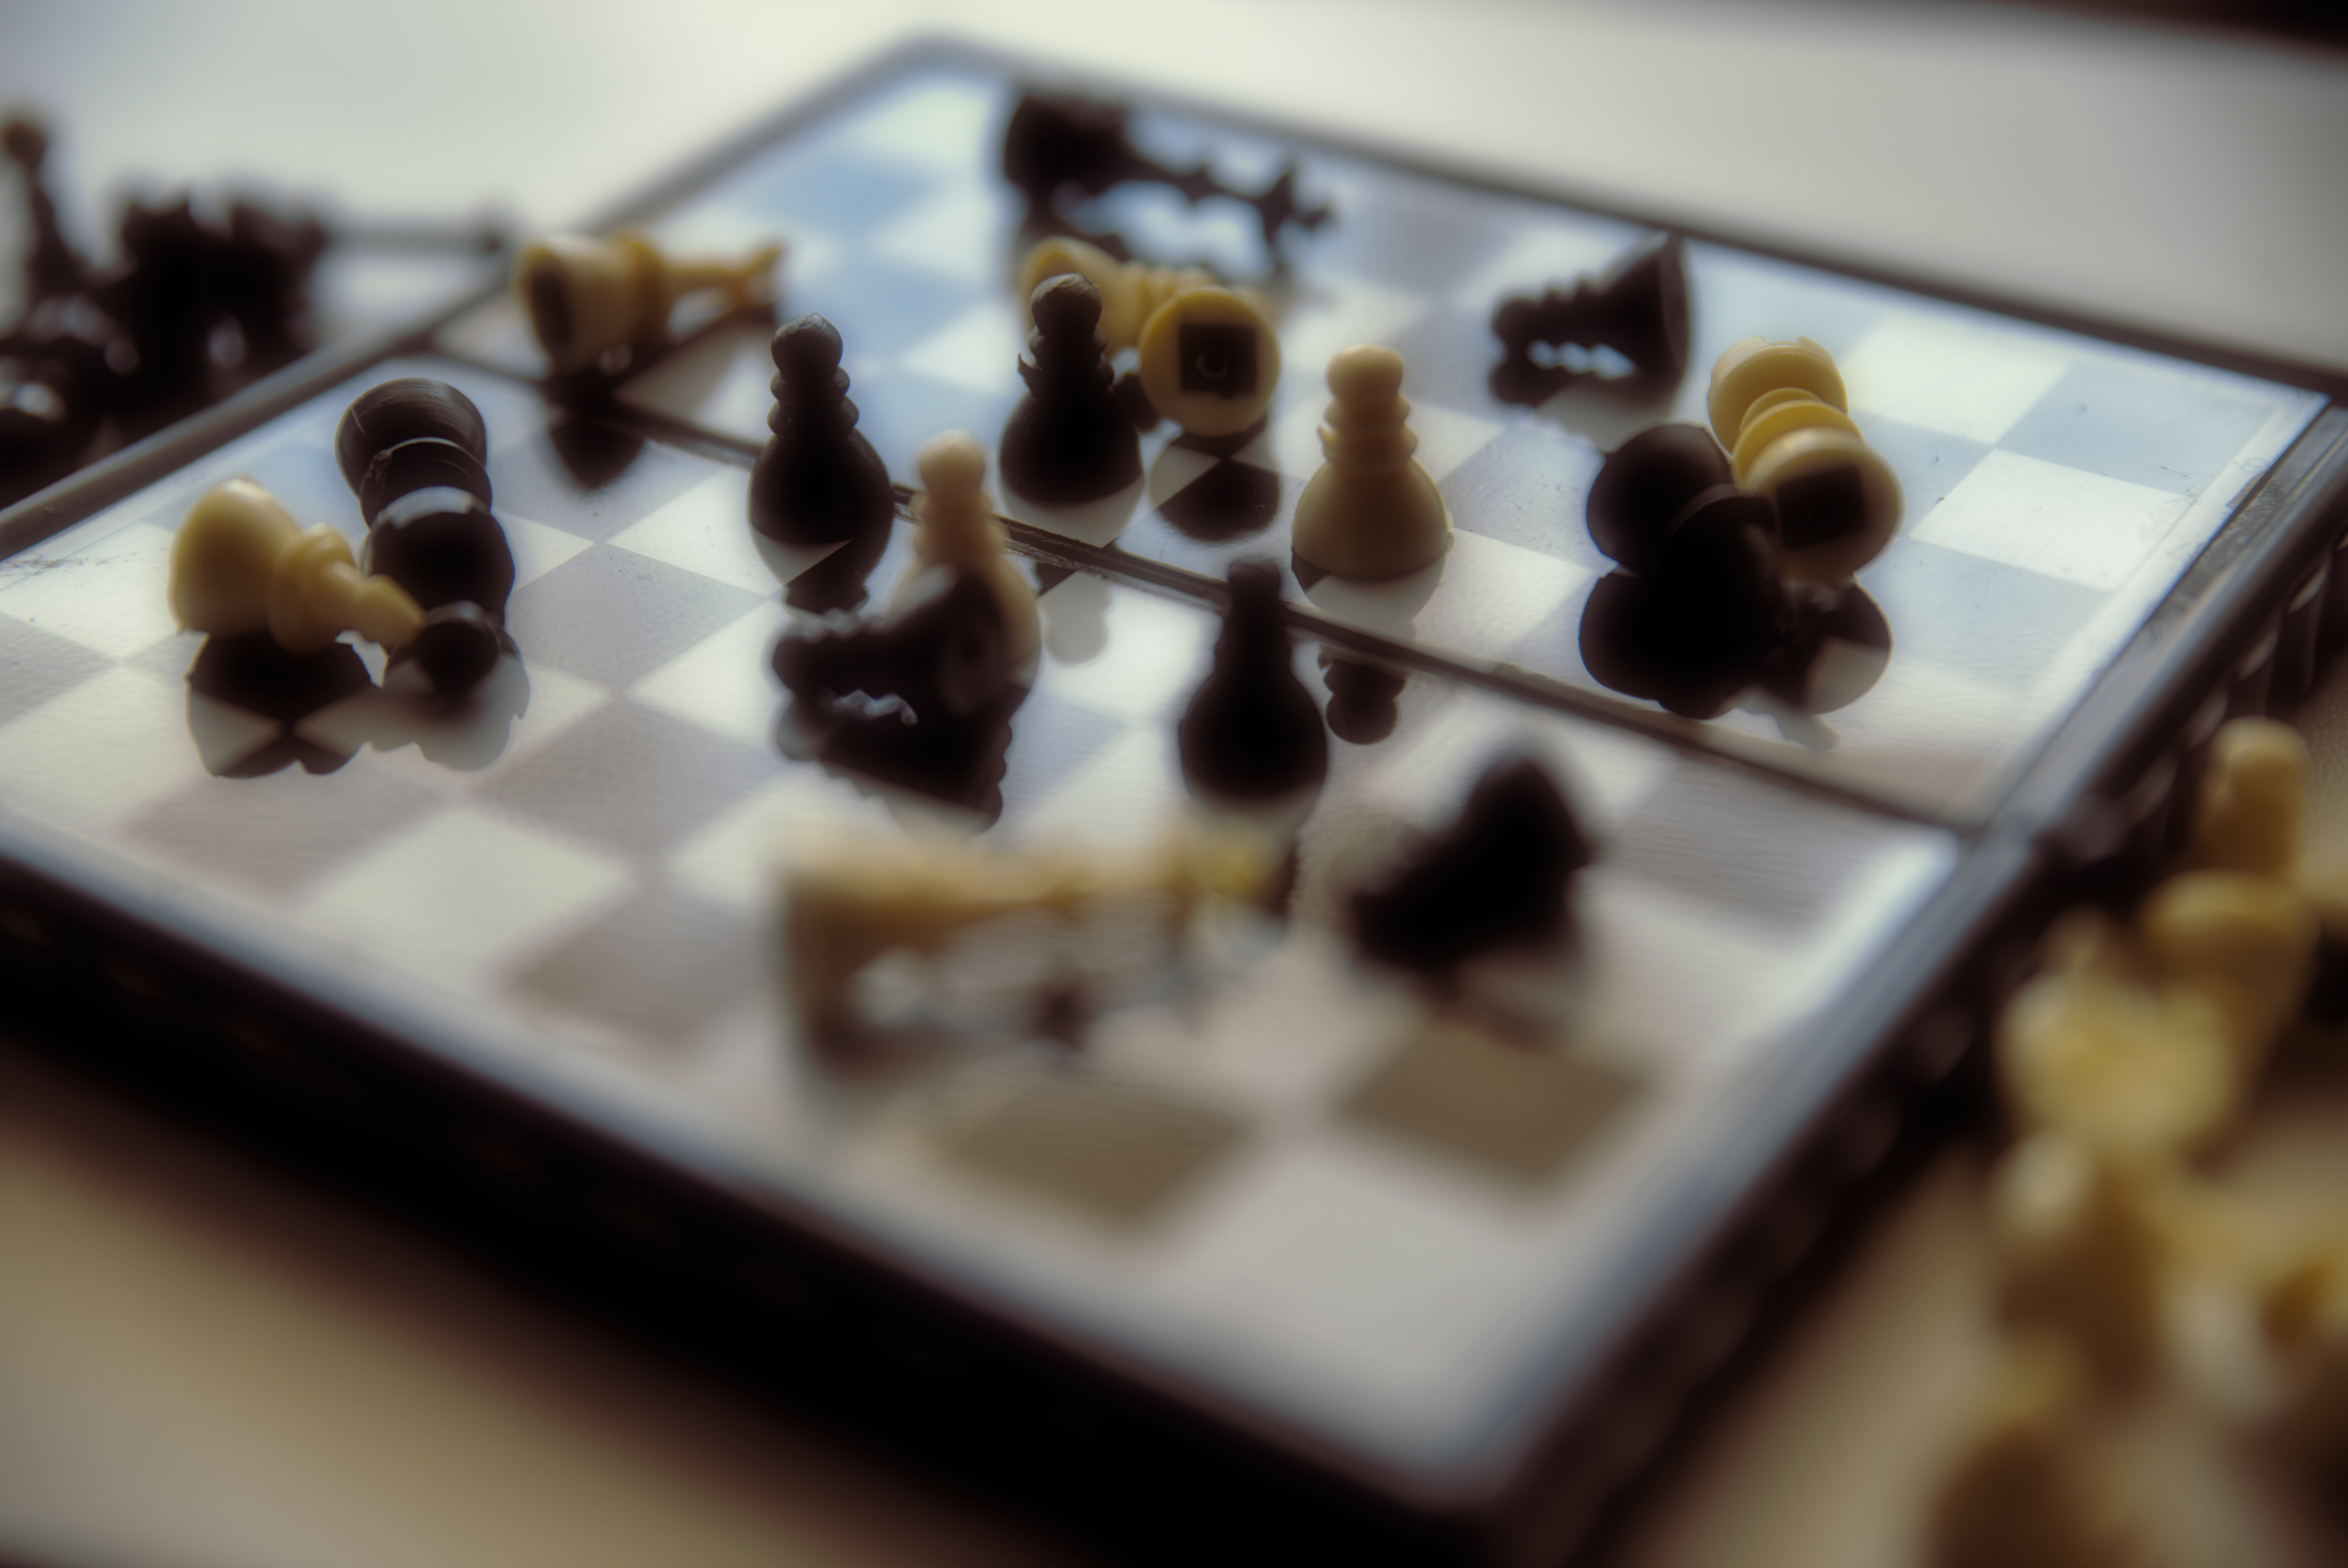
\includegraphics[width=0.9\textwidth, keepaspectratio=true]{../gfx/crochess.jpg} \\ [2.0cm]

    \textbf{\large{Mario Mlačak}} \\ [2.0cm]
\end{center}
\vspace{\stretch{1}}
\end{titlepage}
% ---------------------------------------------------------- Title page

% Empty page ----------------------------------------------------------
\thispagestyle{empty}
\vspace*{0.1\textheight}
\clearpage
% ---------------------------------------------------------- Empty page

% Dedication page -----------------------------------------------------
\thispagestyle{empty}
\vspace*{0.2\textheight}
\hfill{Dedicated to Miranda.}
\clearpage
% ----------------------------------------------------- Dedication page

% Publisher page ------------------------------------------------------
\thispagestyle{empty}
\vspace*{0.1\textheight}
\begin{center}
    \emph{Mario Mlačak} \\
    \textbf{Croatian chess} \\
    and other variants \\ [2.0em]

    \emph{Copyright} \\
    Copyright \copyright \hspace{0.2ex} 2009 -- 2016 Mario Mlačak \\
    \href{mailto:mmlacak@gmail.com}{mmlacak@gmail.com} \\ [2.0em]

    \emph{Legal} \\
    This book is published as Public Domain work. \\
    \href{https://en.wikipedia.org/wiki/Public\_domain}{https://en.wikipedia.org/wiki/Public\_domain} \\ [2.0em]

    \emph{Third, revised edition} \\
    \today \\
    Zagreb

    \vfill

    \LaTeXe
    \vspace{0.1\textheight}
\end{center}
\clearpage
% ------------------------------------------------------ Publisher page

% Inner title page ----------------------------------------------------
\thispagestyle{empty}
\vspace*{0.2\textheight}
\begin{center}
    \textbf{\Large{Croatian chess}} \\ [1.0em]
    \large{and other variants} \\ [1.0em]
    \small{3rd, revised edition} \\ [2.0cm]
    \vspace*{0.2\textheight}

    \textbf{\large{Mario Mlačak}} \\ [1.0em]
    \small{\today} % \\ [2.0cm]
\end{center}
\clearpage
% ---------------------------------------------------- Inner title page

% Empty page ----------------------------------------------------------
\thispagestyle{empty}
\vspace*{0.1\textheight}
\clearpage
% ---------------------------------------------------------- Empty page

% Gratitude page ------------------------------------------------------
\thispagestyle{empty}
\vspace*{0.2\textheight}
\begin{flushright}
My most sincere gratitude to:

Valentina Štefanić \\
Kristina Mlačak \\
Slavko Štefanić

and many, many others.

Thank you all.
\end{flushright}
\clearpage
% ------------------------------------------------------ Gratitude page

% Empty page ----------------------------------------------------------
\thispagestyle{empty}
\vspace*{0.1\textheight}
\clearpage
% ---------------------------------------------------------- Empty page

% Introduction chapter ------------------------------------------------
\chapter*{Introduction}
\addcontentsline{toc}{chapter}{Introduction}

\begin{flushright}
\parbox{0.6\textwidth}{
\emph{Life's too short for chess. \\
\hspace*{\fill}{\textperiodcentered \textperiodcentered \textperiodcentered \hspace*{0.2em} Henry James Byron} } }
\end{flushright}

I was in my aunt's house, on the border of a small village.
Through window walled garden and small brook was visible just
behind the house. And hills in the distance. Early afternoon Sun
was casting its orange rays into warm room. It was cold outside.

My cousin approached me with some nifty gizmo. He was a
few years older then me and was already going to school. \\
"Here, look at what I got." \\
"What's that?" \\
"Chess set. Wanna try? Lemme show you." \\
"Sure."

It was small plasticky, fiddly thing designed to fit into winter's
coat pocket, to be used on the go. Folding board was also used to
hold all pieces in it. Each piece was as small as humanely usable.
Each field had a hole in the middle. Bellow each piece there was
small rod fitting into those holes. It was colored all in red and ivory.

Short lesson revealed it's not that difficult to grasp what's going
on. Within minutes I picked it up. First match was, predictably, a
complete disaster. On the second go my cousin forgot about a piece,
and I grabbed his Queen gleefully. He surrendered.

After he left me with a new widget, I was intrigued. I wasn't
about playing the game, though. I was more into redesign it. Could it
be made better, more challenging, or just different? \\
'Why not make Knight jump longer, say 3 by 1 fields?' \\
'Hmmmm...' \\
'Nah, that would make jump too long for such a small board.'

Outside, the Sun was shining red.
\clearpage
% ------------------------------------------------ Introduction chapter

% Prerequisites chapter -----------------------------------------------
\chapter*{Prerequisites}
\addcontentsline{toc}{chapter}{Prerequisites}

\begin{flushright}
\parbox{0.7\textwidth}{
\emph{It does not matter how slowly you go as long as you do not stop. \\
\hspace*{\fill}{\textperiodcentered \textperiodcentered \textperiodcentered \hspace*{0.2em} Confucius} } }
\end{flushright}

This document describes new variants of chess, new pieces
and rules. In this document I'll describe only even variants, since
generating odd ones from there is an exercise in simplicity. Please,
see 'Even variant', 'Odd variant' in the Definitions bellow.

\textbf{\huge{TODO :: FIX ME !!!}} % TODO :: FIX ME !!!

In this document I'm assuming you have the complete prior
knowledge of classical chess pieces and rules. If not, please visit
Wikipedia entry on this subject at \\
\href{https://en.wikipedia.org/wiki/Rules\_of\_chess}{https://en.wikipedia.org/wiki/Rules\_of\_chess}.
\clearpage
% ----------------------------------------------- Prerequisites chapter

% Classical Game chapter ----------------------------------------------
\chapter*{Classical Game}
\addcontentsline{toc}{chapter}{Classical Game}

\begin{flushright}
\parbox{0.8\textwidth}{
\emph{A great war leaves the country with three armies -
an army of cripples, an army of mourners, and an army of thieves. \\
\hspace*{\fill}{\textperiodcentered \textperiodcentered \textperiodcentered \hspace*{0.2em} German proverb} } }
\end{flushright}

About classical chess is written really everything already, and I
have nothing to add. Except for illustration of initial setup, so that
you can accustom yourself with rendition of pieces used in this text.

Note that in Odd Classical Game, since it's played on 7 x 7 board,
there is no en-passant move. This is so because of very small board
there is no room for a Pawn to perform 2-field initial move without,
at the same time, preventing opponent to do the same at the same file.

\noindent
\begin{figure}[t]
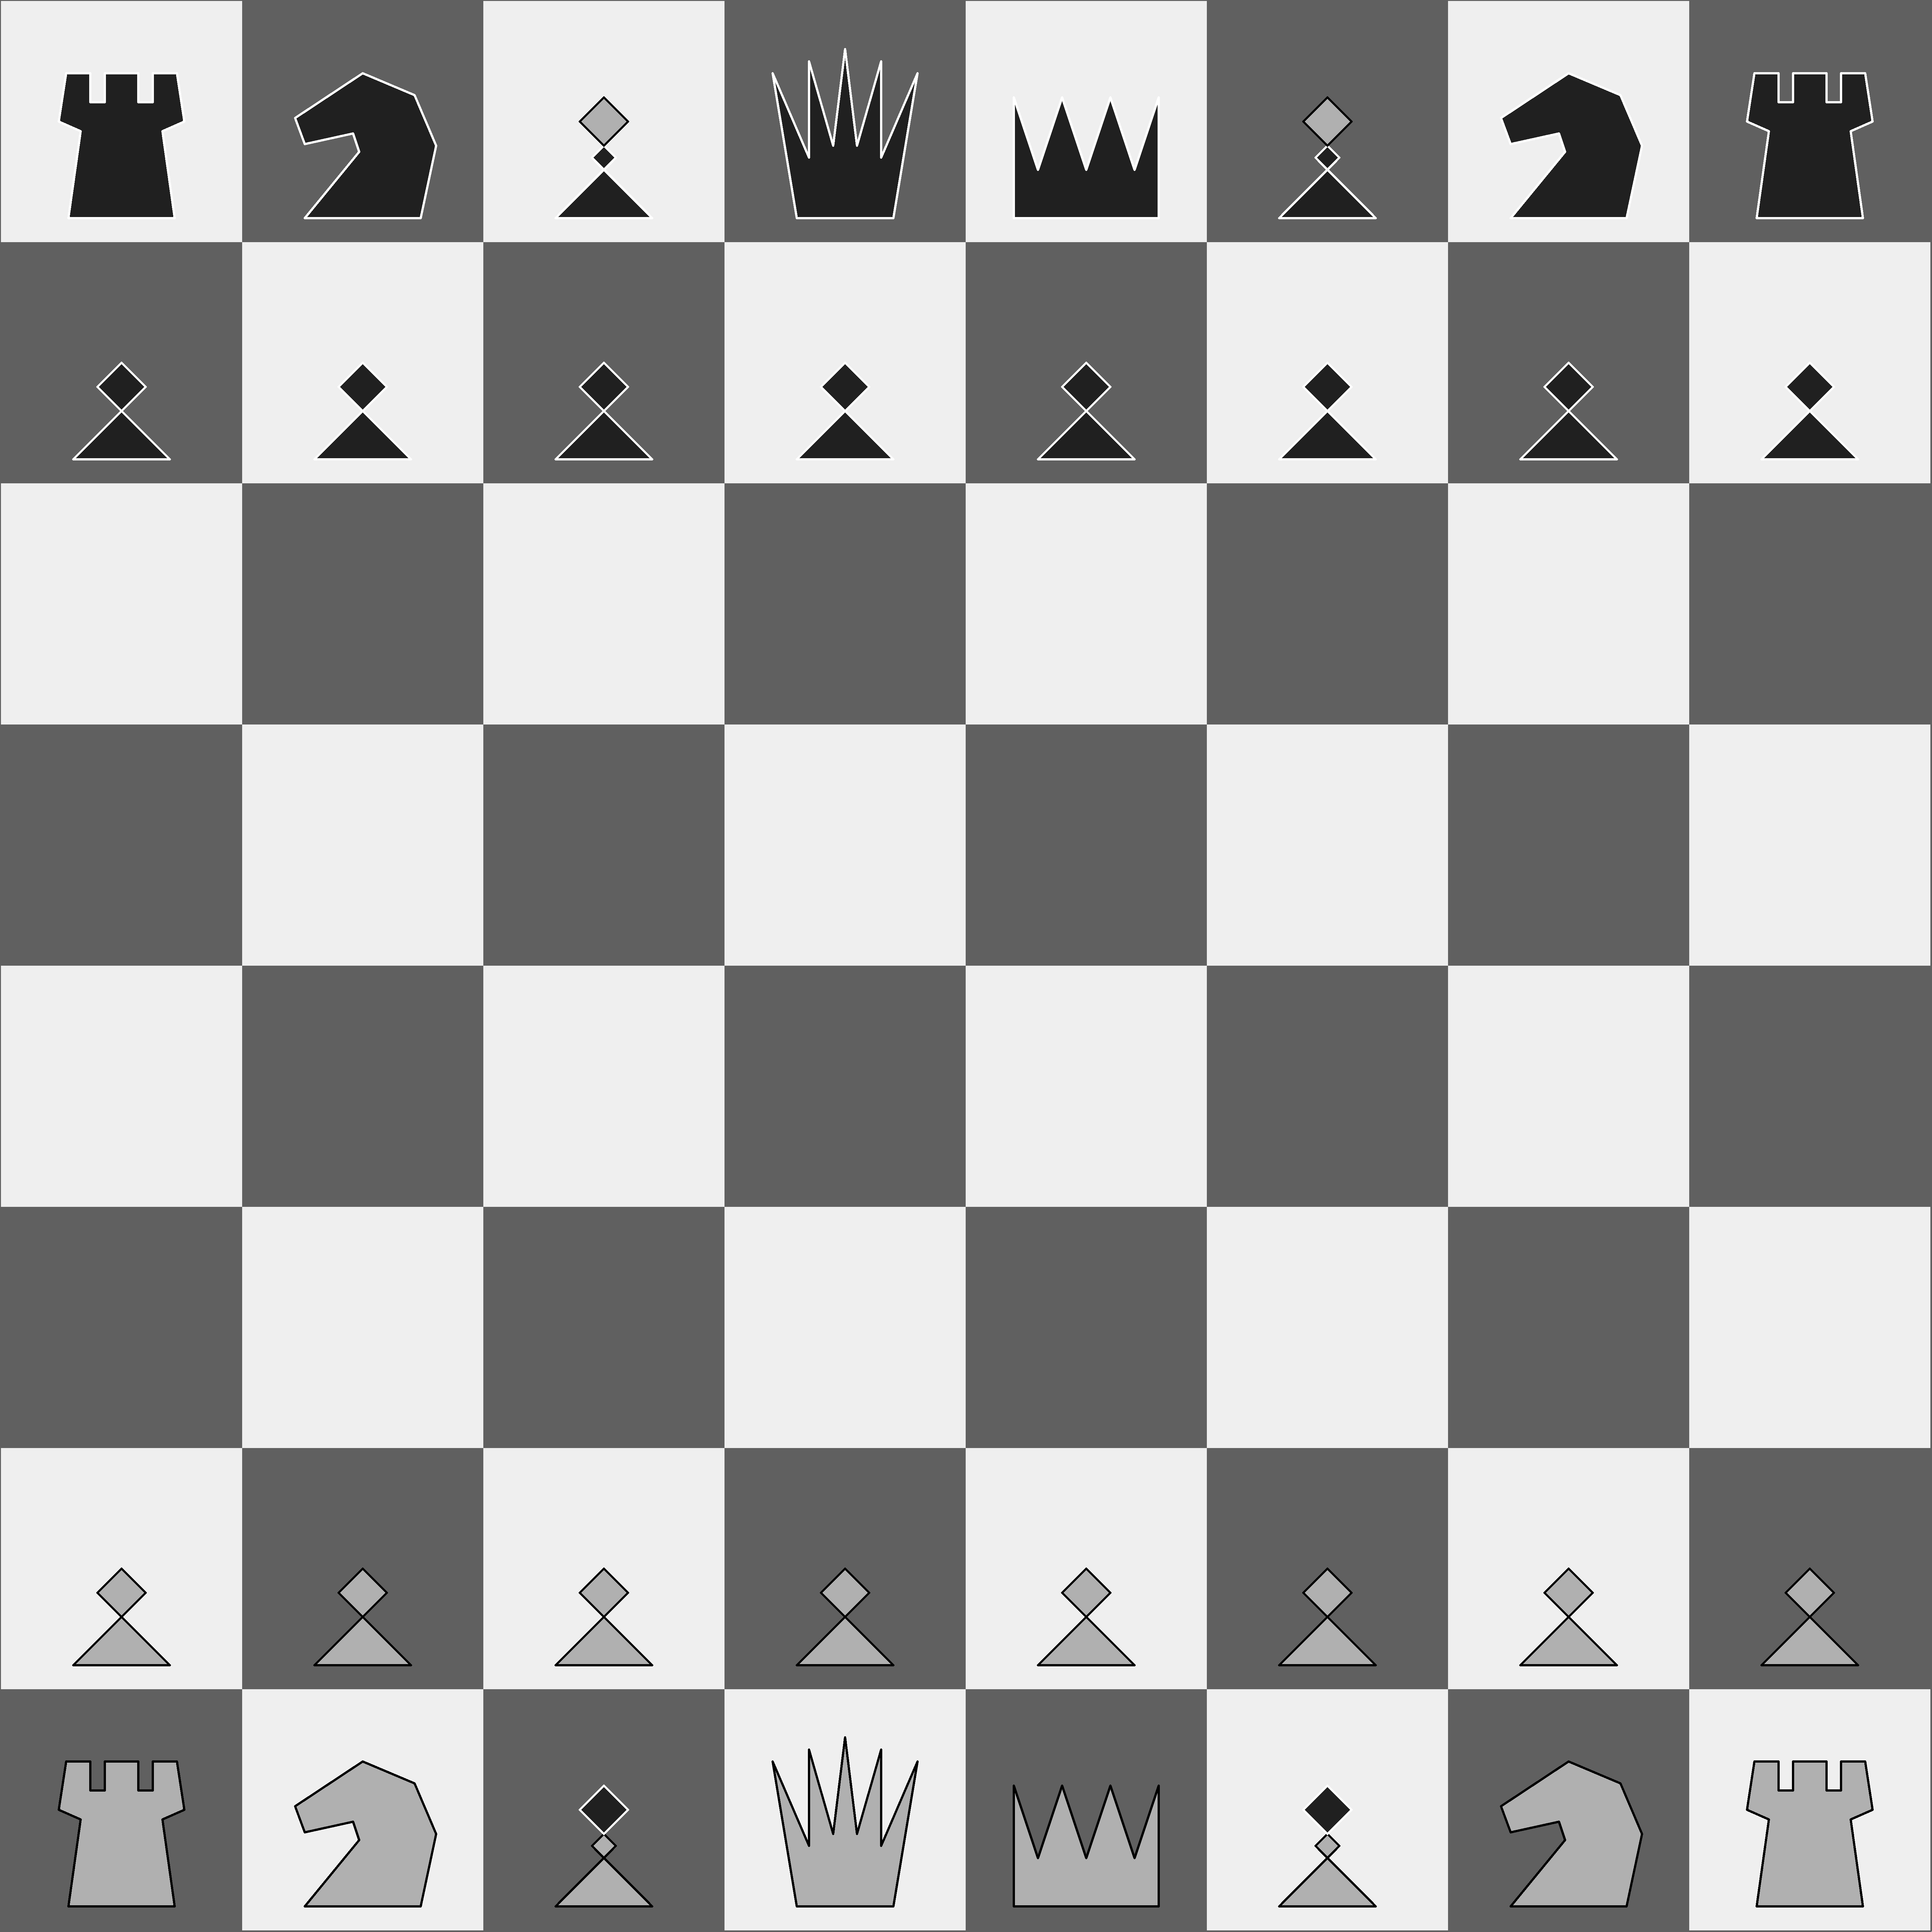
\includegraphics[width=1.0\textwidth, keepaspectratio=true]{../gfx/boards/02_classical.png}
\caption{Classical board}
\label{fig:classical_chess}
% \centering
\end{figure}

\clearpage
% ---------------------------------------------- Classical Game chapter

% Croatian Ties chapter -----------------------------------------------
\chapter*{Croatian Ties}
\addcontentsline{toc}{chapter}{Croatian Ties}

\begin{flushright}
\parbox{0.7\textwidth}{
\emph{Secrecy is the first essential in affairs of the State. \\
\hspace*{\fill}{\textperiodcentered \textperiodcentered \textperiodcentered \hspace*{0.2em} De Richelieu} } }
\end{flushright}

Croatian Ties is chess variant which is played on 10 x 10 board,
with silver and red fields and dark silver and dark red pieces.
In algebraic notation, columns are enumerated from 'a' to 'j',
and rows are enumerated from '1' to '10'. A new piece is
introduced, Pegasus.

\clearpage

\section*{Pegasus}
\addcontentsline{toc}{section}{Pegasus}

\noindent
\begin{wrapfigure}[10]{l}{0.4\textwidth}

\includegraphics[width=0.4\textwidth, keepaspectratio=true]{../gfx/pieces/07_pegasus.png}
\caption{Pegasus}
\label{fig:pegasus}
% % \centering
\end{wrapfigure}
\indent
Pegasus moves similarly to Knight, but it can continue its jumpy movement
until another piece is encountered, or it runs out of board. Note that once
in movement, Pegasus can not change its' heading.

Pegasus symbol in algebraic notation is 'G', to avoid confusion with Pawn.

\vspace{1\baselineskip}

\noindent
\begin{wrapfigure}[11]{l}{0.5\textwidth}
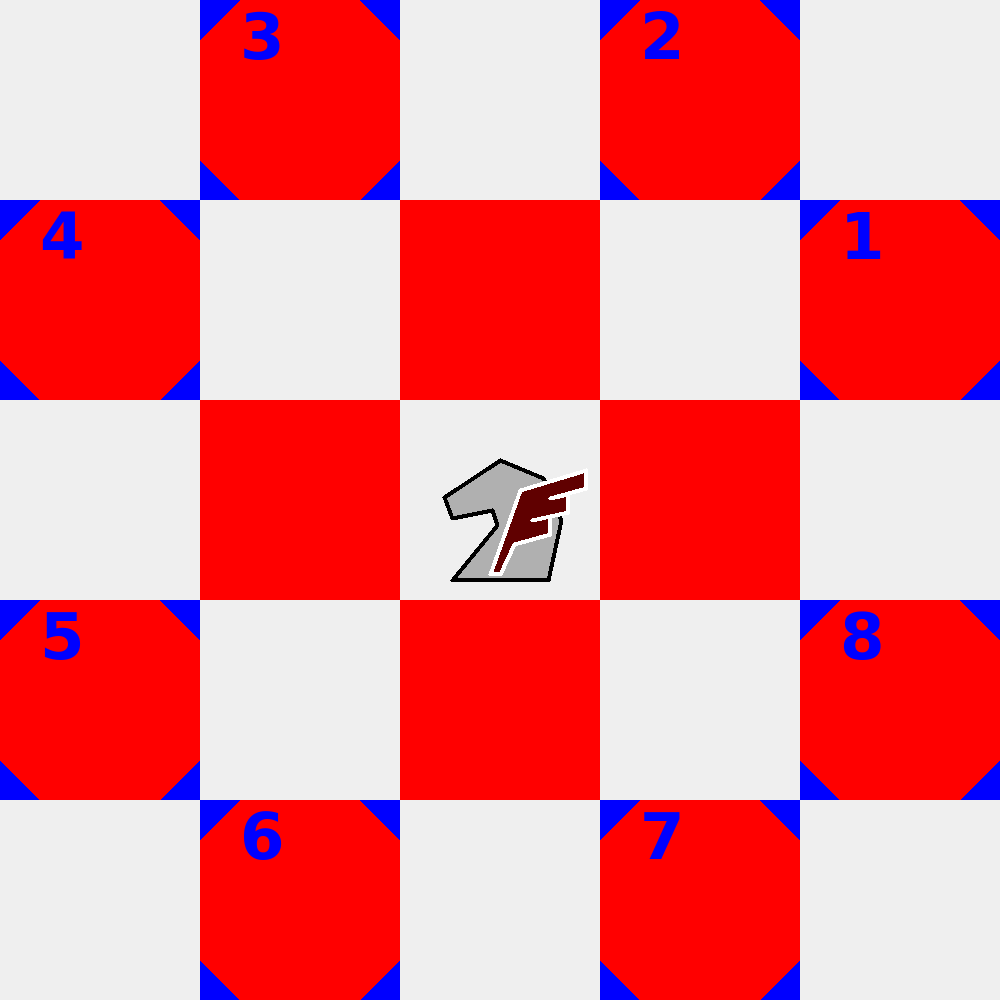
\includegraphics[width=0.5\textwidth, keepaspectratio=true]{../gfx/examples/01_move_pegasus_initial.png}
\caption{Pegasus initial step}
\label{fig:pegasus_initial_step}
% % \centering
\end{wrapfigure}
\indent
In the example on the left we have Pegasus with all valid initial move directions
marked with green arrows. Each accessible field has number in its' corner.
Pegasus' movement is not hampered by surrounding pieces (in this case own Pawns),
it can "jump" over them just as Knight would.

\clearpage

\noindent
% \begin{figure}[t]
\begin{figure}[!t]
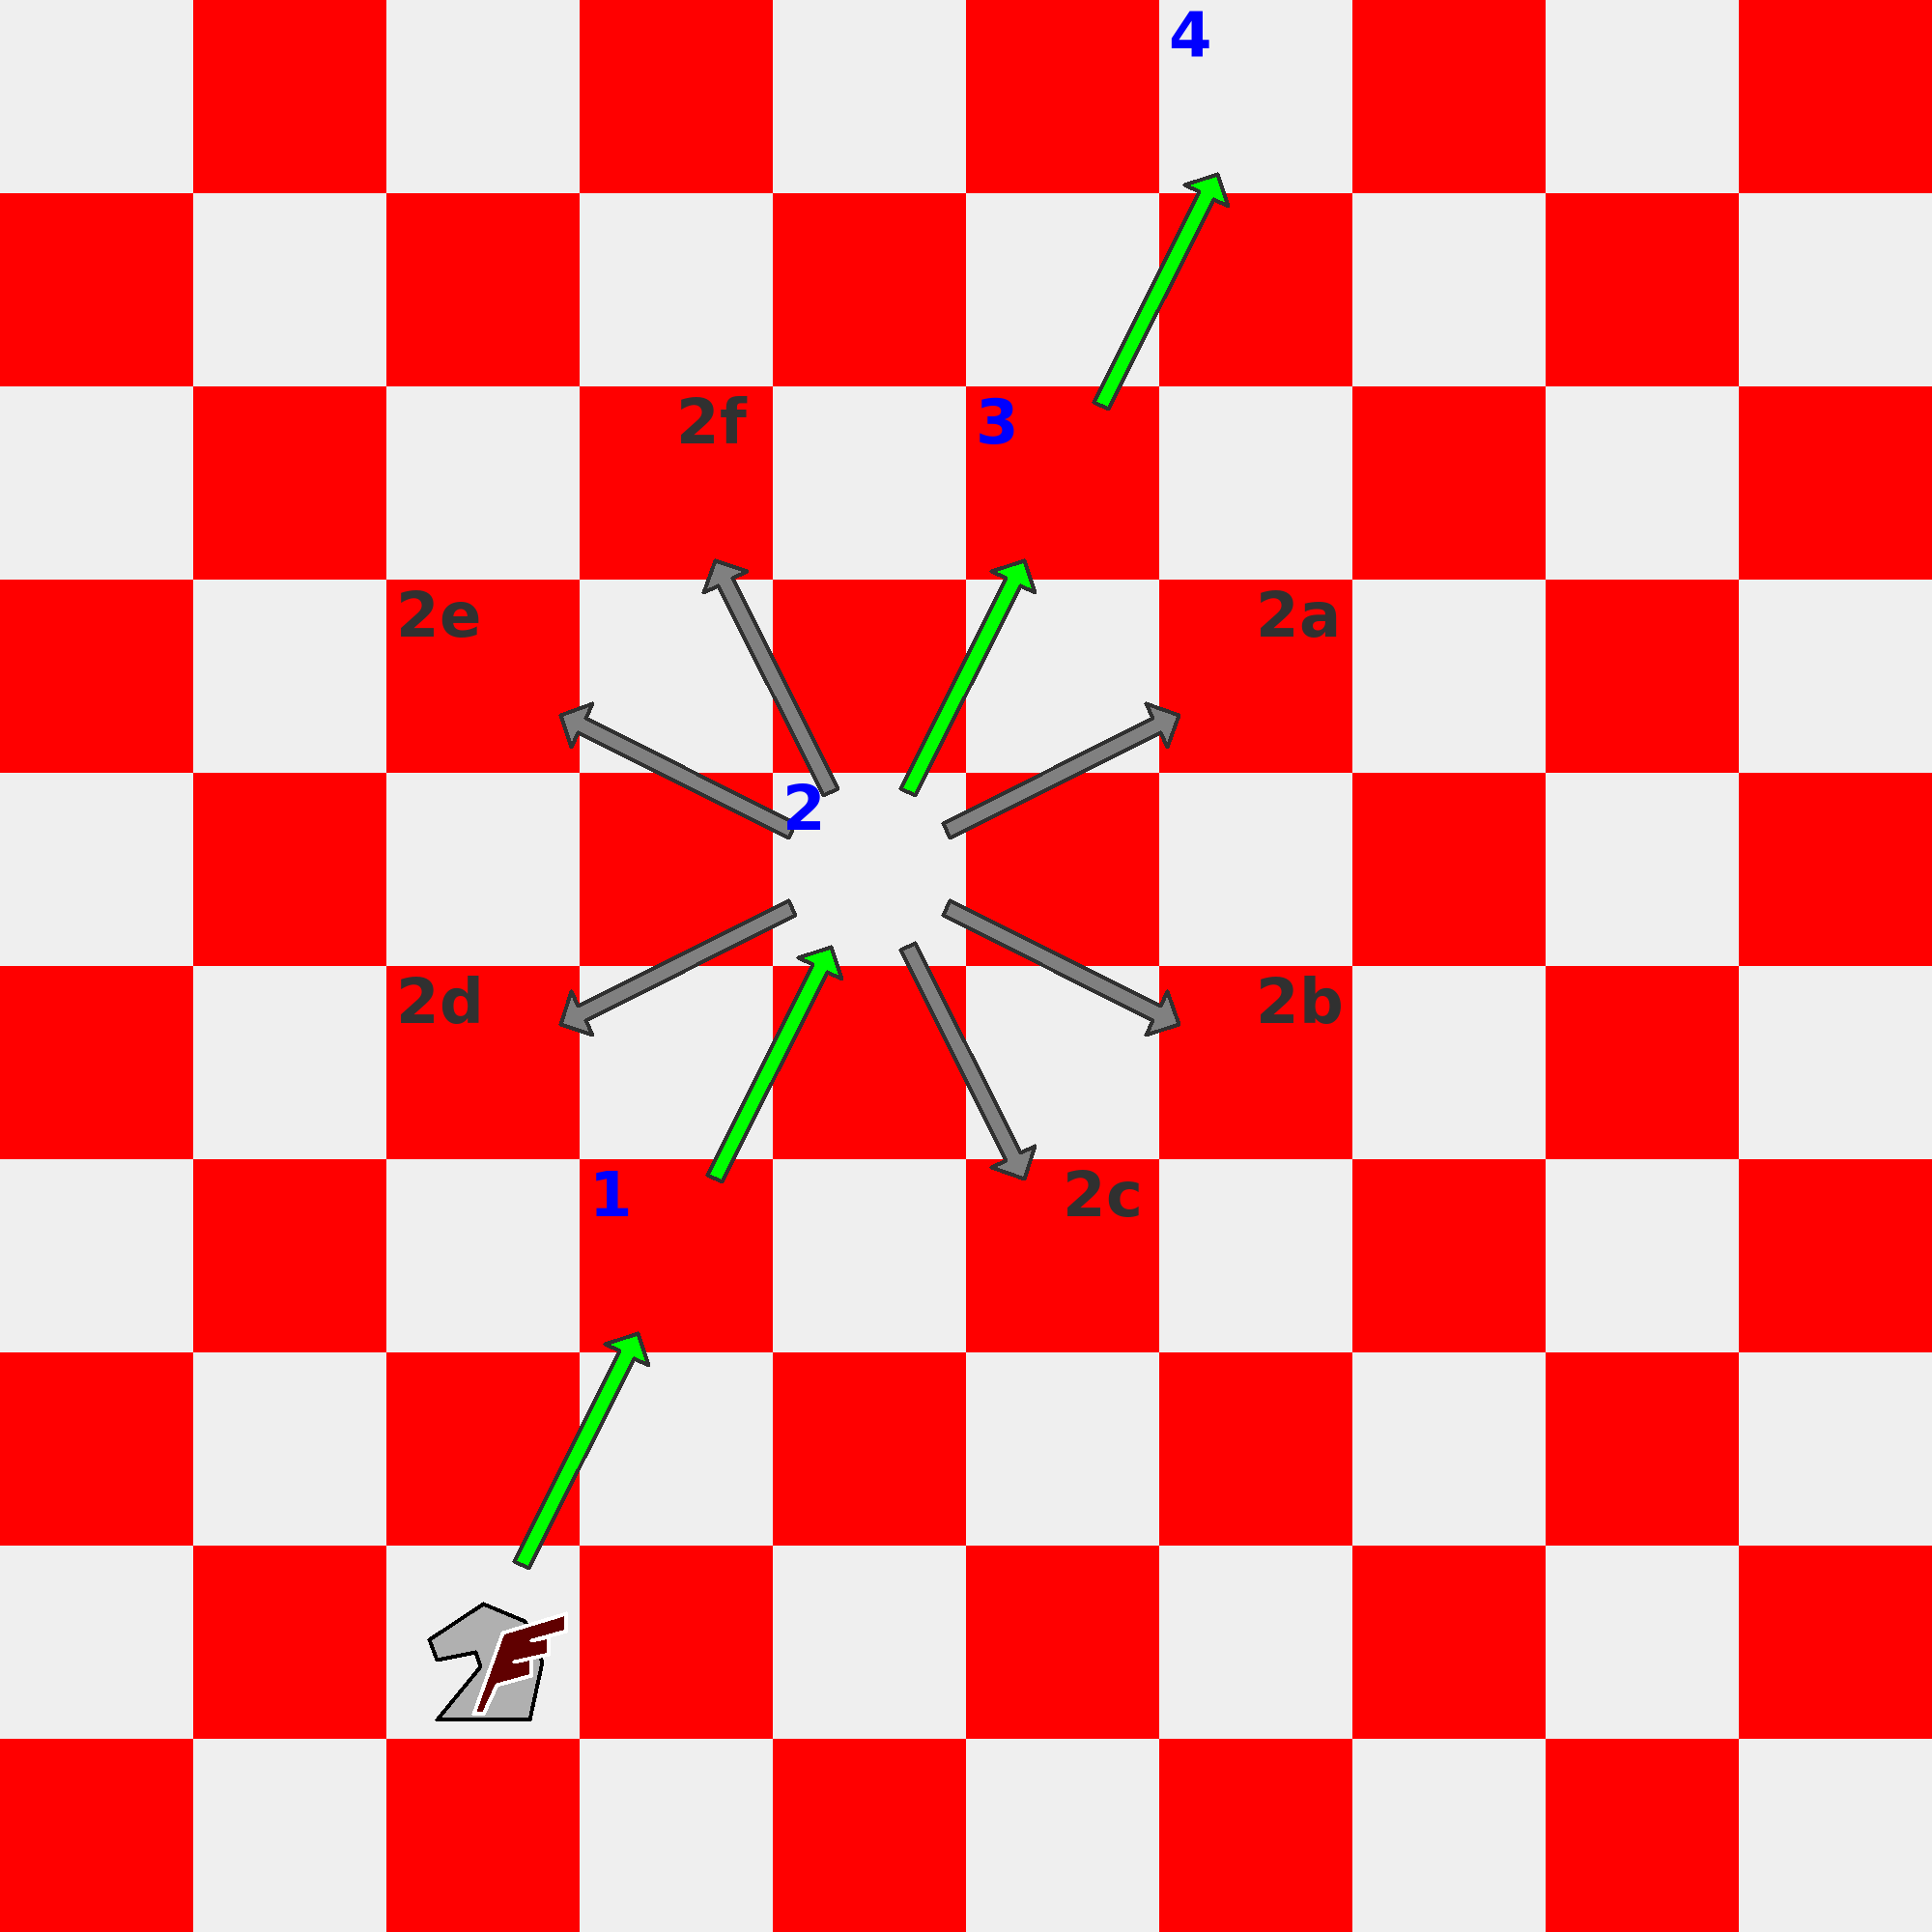
\includegraphics[width=1.0\textwidth, keepaspectratio=true]{../gfx/examples/02_move_pegasus_direction.png}
\caption{Pegasus move direction}
\label{fig:pegasus_move_direction}
% \centering
\end{figure}
\indent
Once direction is chosen Pegasus can continue its' movement performing one jump
after another in order from nearest field to furthest. Here, this is marked
with green arrows. Accessible fields are marked 1 to 4, in order of accessibility,
from nearest to furthest. Again, once direction is chosen it can't be changed
anymore. For instance, after reaching field 2 it's not allowed to change
direction to 2f (or any other greyed-out arrow).

\clearpage

\noindent
% \begin{figure}[t]
\begin{figure}[!t]
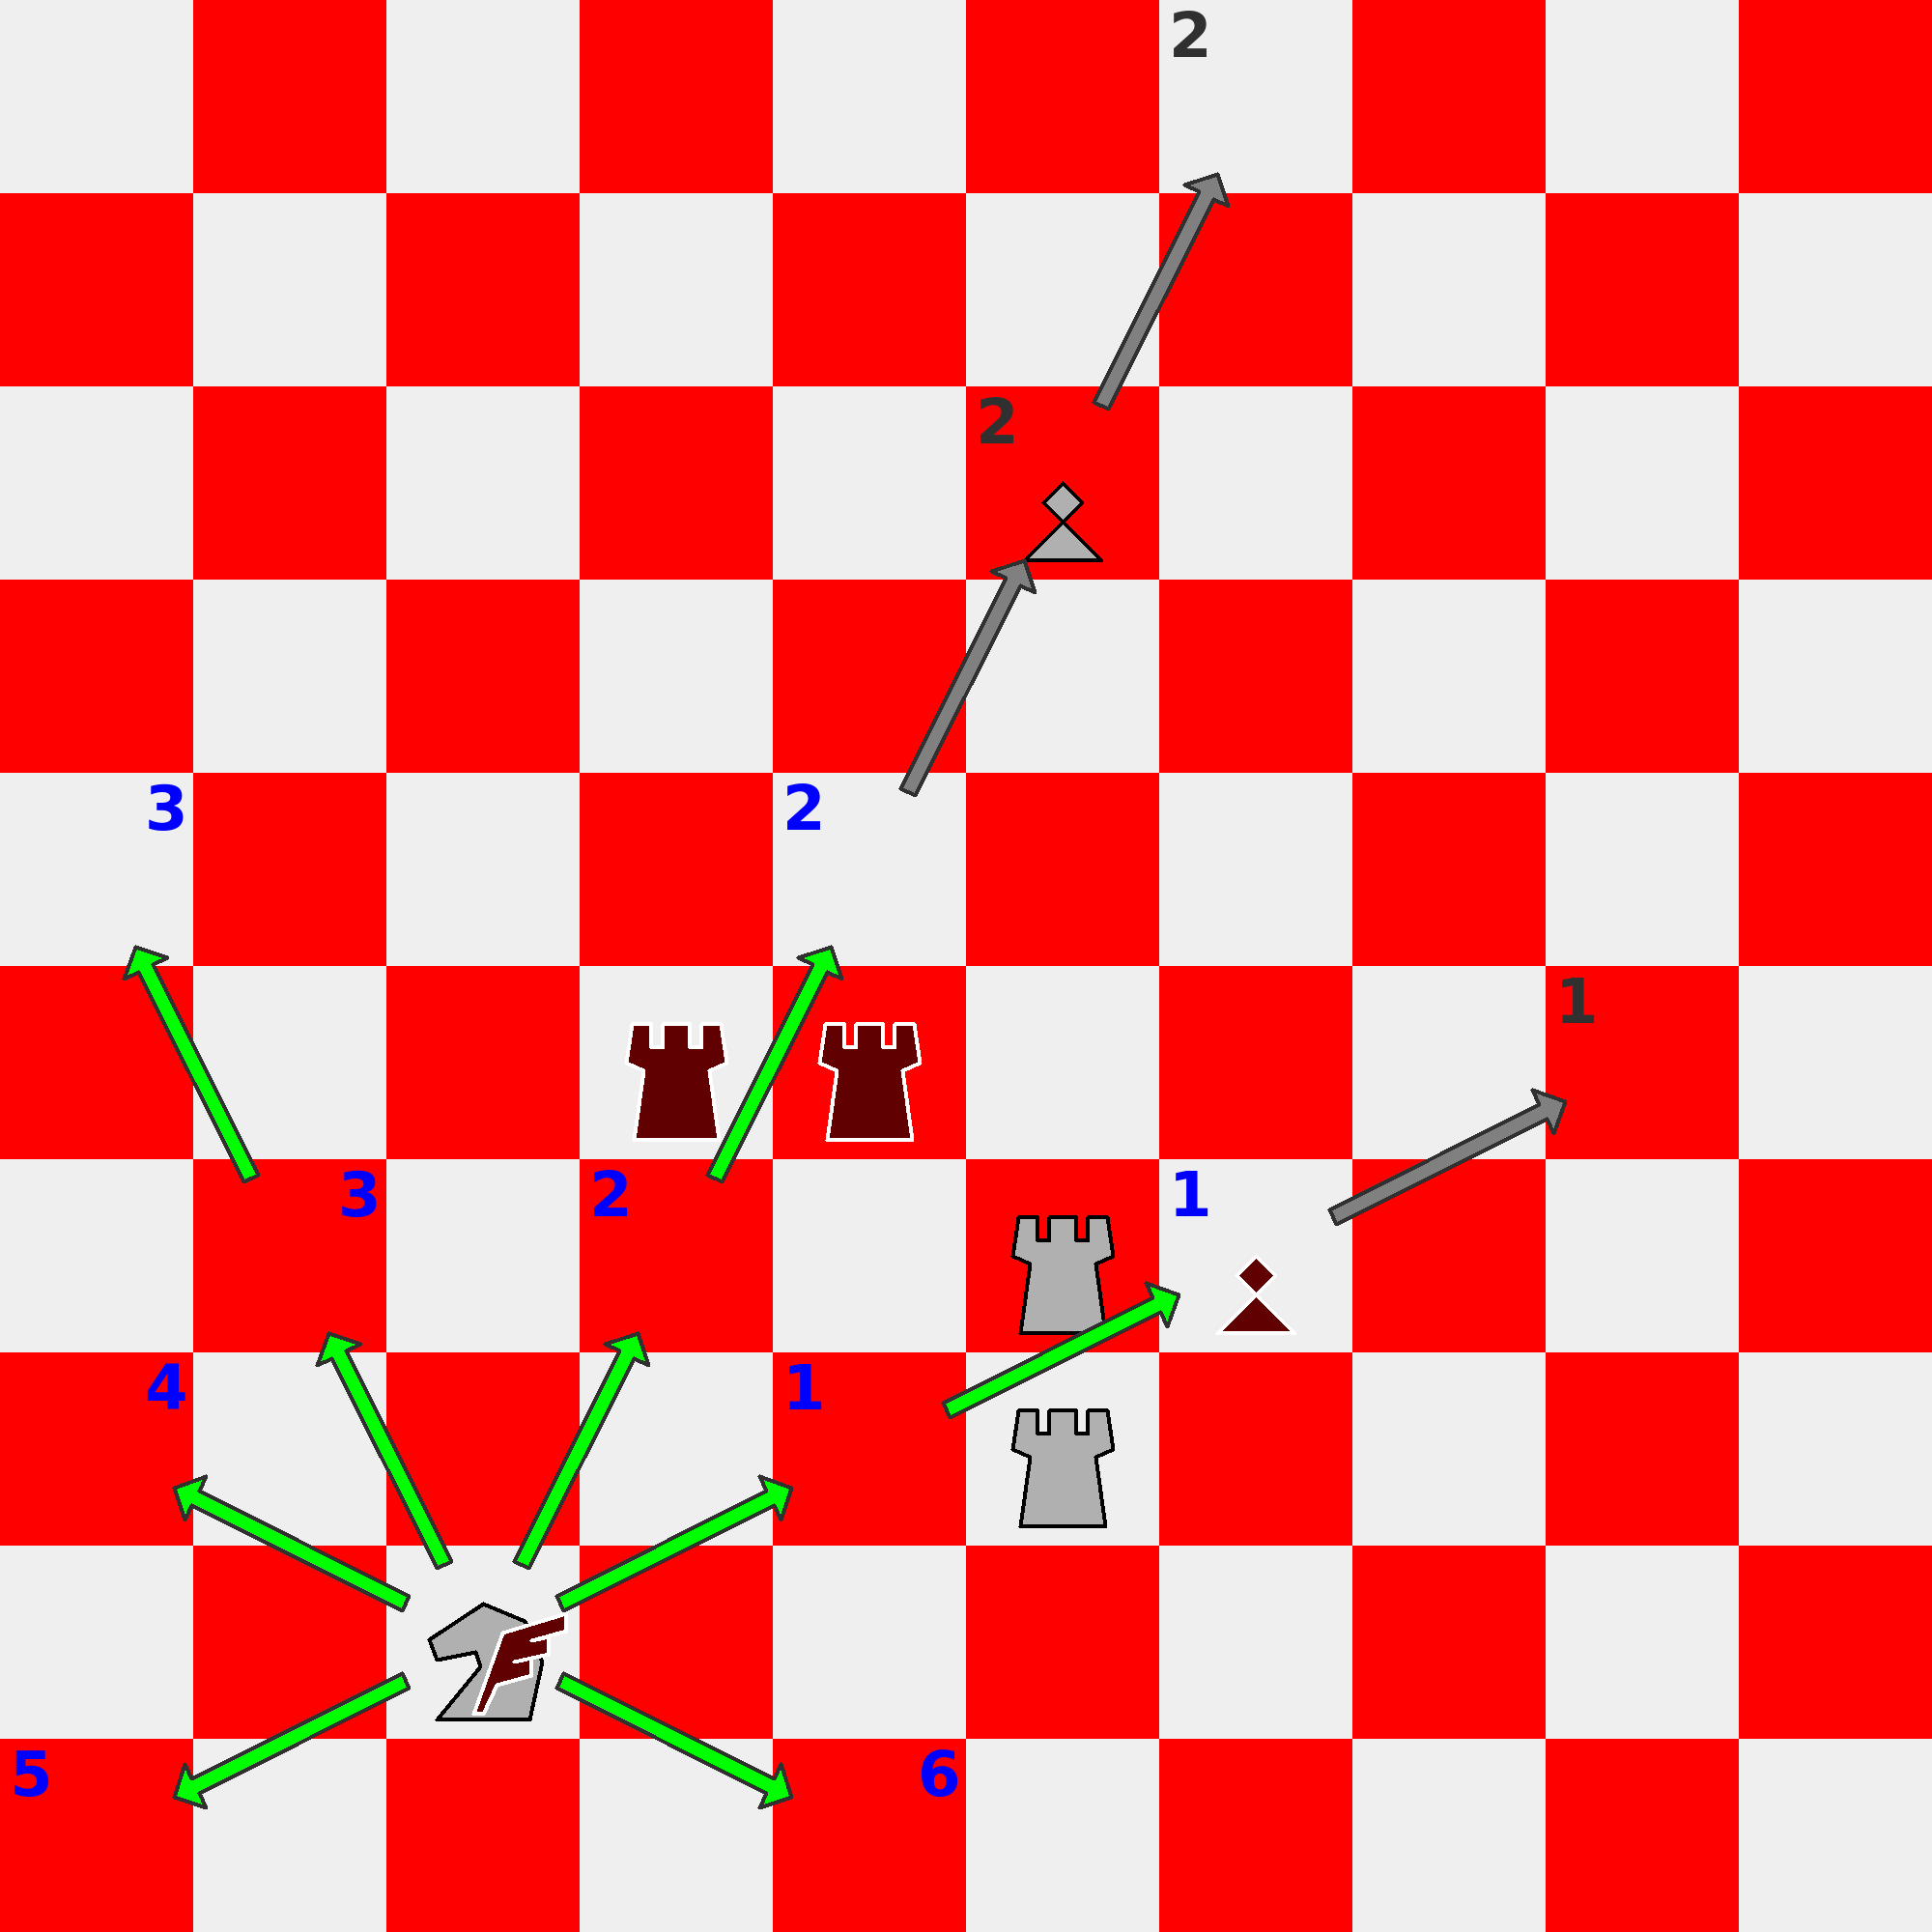
\includegraphics[width=1.0\textwidth, keepaspectratio=true]{../gfx/examples/03_move_pegasus.png}
\caption{Pegasus moves}
\label{fig:pegasus_moves}
% \centering
\end{figure}
\indent
Move along arrow is called step. Field at which arrow points to is called step field.
Pegasus can "jump" over pieces on non-step fields, Rooks in example above. Numbers
here enumerate directions of movement. Own piece on step field stops Pegasus at
preceding step field, see direction 2. Opponent's piece on step field can be captured,
just as with any other piece that would finish the move, meaning Pegasus would have to
stop at captured step field.

\clearpage

\section*{En passant}
\addcontentsline{toc}{section}{En passant}

\noindent
\begin{wrapfigure}{l}{0.4\textwidth}
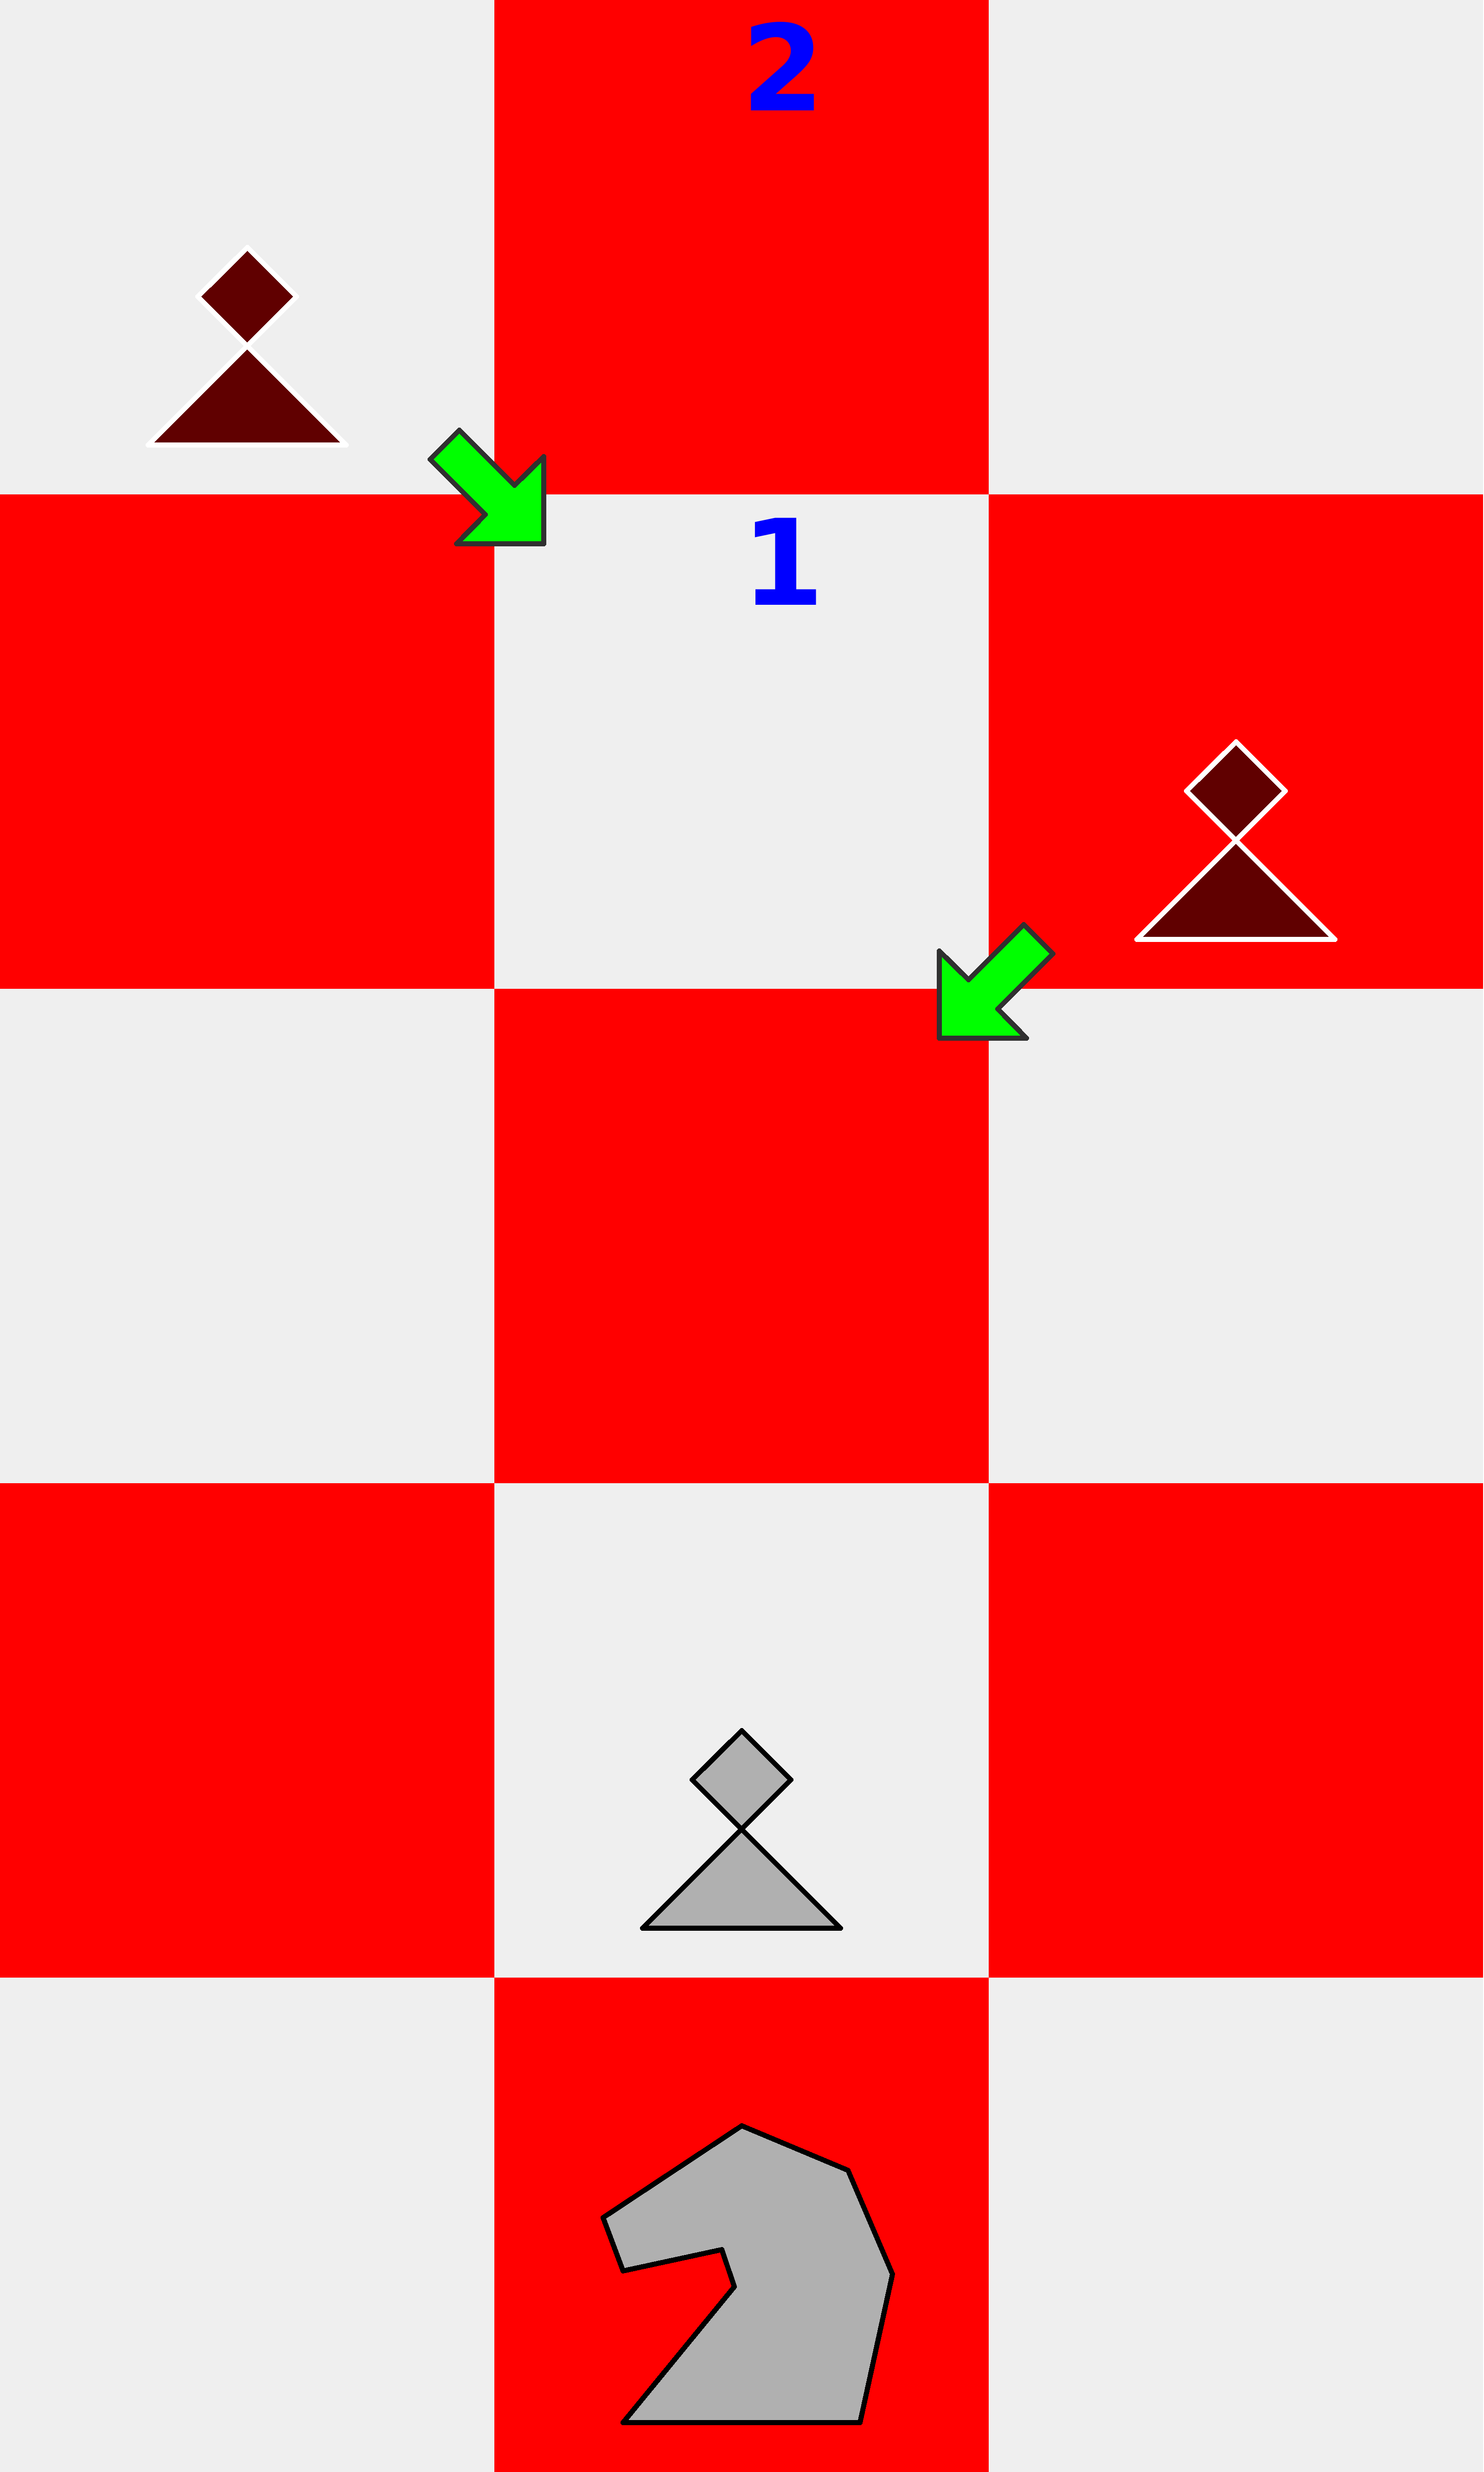
\includegraphics[width=0.4\textwidth, keepaspectratio=true]{../gfx/en_passants/04_croatian_ties_en_passant.png}
\caption{En passant}
\label{fig:cc_en_passant}
% % \centering
\end{wrapfigure}
\indent
If Pawn hasn't moved yet, it can move up to 3 fields forward. As expected, all passed-by
opponent's Pawns also gain en passant opportunity.

In example on left, if light Pawn's
initial move was 3 fields long, ending in field marked 2, both dark Pawns would have en
passant opportunity. Naturaly, if initial move was only 2 fields long, ending in field
marked 1, only dark Pawn on the right would gain en passant opportunity.

\clearpage

\section*{Castling}
\addcontentsline{toc}{section}{Castling}

\indent
Castling is essentially the same as it is in Classical Chess, only real difference is that
King can move either 2 or 3 fields across. All other constraints from Classical Chess still
applies, described in detail here \\
\href{https://en.wikipedia.org/wiki/Castling}{https://en.wikipedia.org/wiki/Castling}.

\noindent
\begin{figure}[!h]
% \begin{figure}[!t]

\includegraphics[width=1.0\textwidth, keepaspectratio=true]{../gfx/castlings/04_croatian_ties_castling.png}
\caption{Castling}
\label{fig:cc_castling}
% \centering
\end{figure}

\indent
In example above, all valid King's castling moves are numbered. Regardless if King performs
long or short castling move, Rook would always end up on field next to King, on opposite side
of it, i.e. closer to center.

\noindent
\begin{figure}[!h]
% \begin{figure}[!t]

\includegraphics[width=1.0\textwidth, keepaspectratio=true]{../gfx/castlings/long_left/04_croatian_ties_castling_long_left.png}
\caption{Castling long left}
\label{fig:cc_castling_long_left}
% \centering
\end{figure}

\indent
In this example King was castling long to the left. Initial King's position is marked with "K".
After castling is finished, left Rook ends up at field immediately on the right to the King.

\clearpage

\section*{Initial setup}
\addcontentsline{toc}{section}{Initial setup}

Initial setup for Light player is (mirrored for Dark one):
\texttt{PPPPPPPPPP \\
        RGNBQKBNGR}, \\
or more conveniently, as seen in this image:

\noindent
% \begin{figure}[t]
\begin{figure}[h]
\includegraphics[width=1.0\textwidth, keepaspectratio=true]{../gfx/boards/04_croatian_ties.png}
\caption{Croatian Ties board}
\label{fig:croatian_ties}
% \centering
\end{figure}

\clearpage
% ----------------------------------------------- Croatian Ties chapter

% Mayan Ascendancy chapter --------------------------------------------
\chapter*{Mayan Ascendancy}
\addcontentsline{toc}{chapter}{Mayan Ascendancy}

\begin{flushright}
\parbox{0.8\textwidth}{
\emph{The world has achieved brilliance without wisdom, power without
conscience. Our is a world of nuclear giants and ethical infants. \\
\hspace*{\fill}{\textperiodcentered \textperiodcentered \textperiodcentered \hspace*{0.2em} Omar Nelson Bradley} } }
\end{flushright}

Mayan Ascendancy is chess variant which is played on 12 x 12 board with
yellow and blue fields and with dark yellow and dark blue pieces. In
algebraic notation, columns are enumerated from 'a' to 'l', and rows are
enumerated from '1' to '12'. A new piece is introduced, Pyramid.

\clearpage

\section*{Pyramid}
\addcontentsline{toc}{section}{Pyramid}

\noindent
\begin{wrapfigure}{l}{0.4\textwidth}
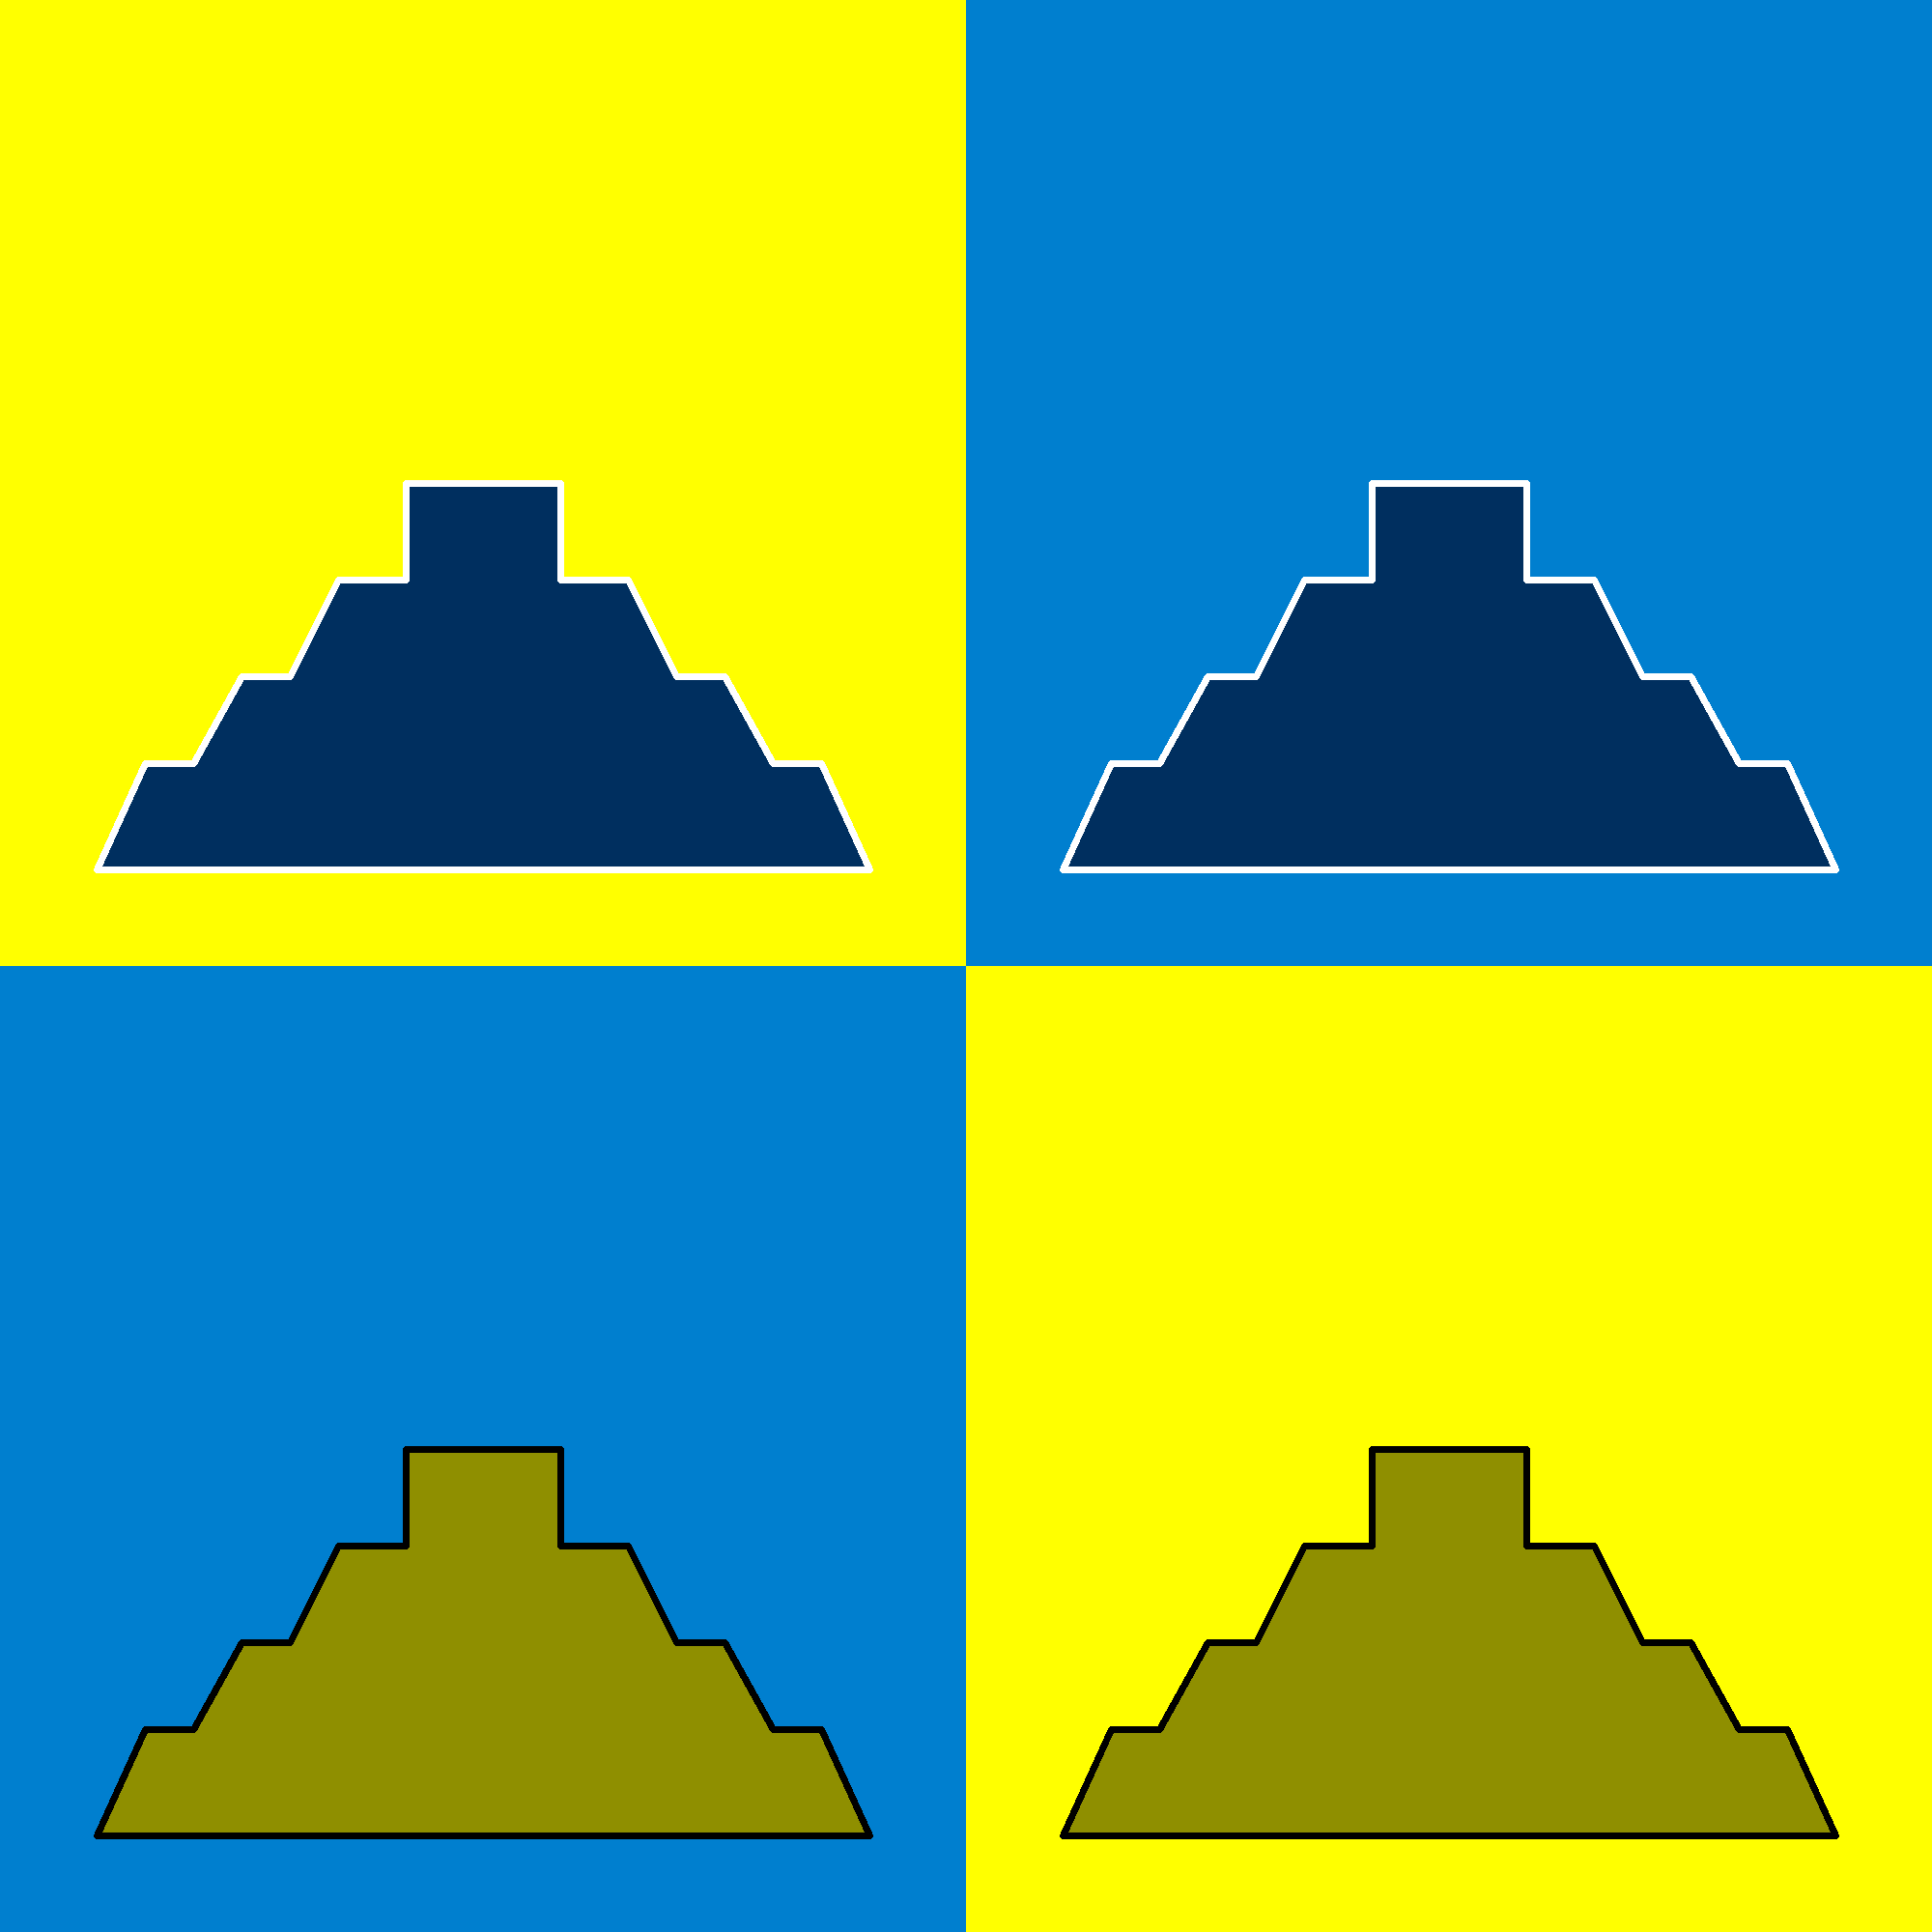
\includegraphics[width=0.4\textwidth, keepaspectratio=true]{../gfx/pieces/08_pyramid.png}
\caption{Pyramid}
\label{fig:pyramid}
% % \centering
\end{wrapfigure}

\clearpage

\section*{Initial setup}
\addcontentsline{toc}{section}{Initial setup}

Initial setup for Light player is (mirrored for Dark one):
\texttt{PPPPPPPPPPPP \\
        RGANBQKBNAGR}, \\
or more conveniently, as seen in this image:

\noindent
% \begin{figure}[t]
\begin{figure}[h]
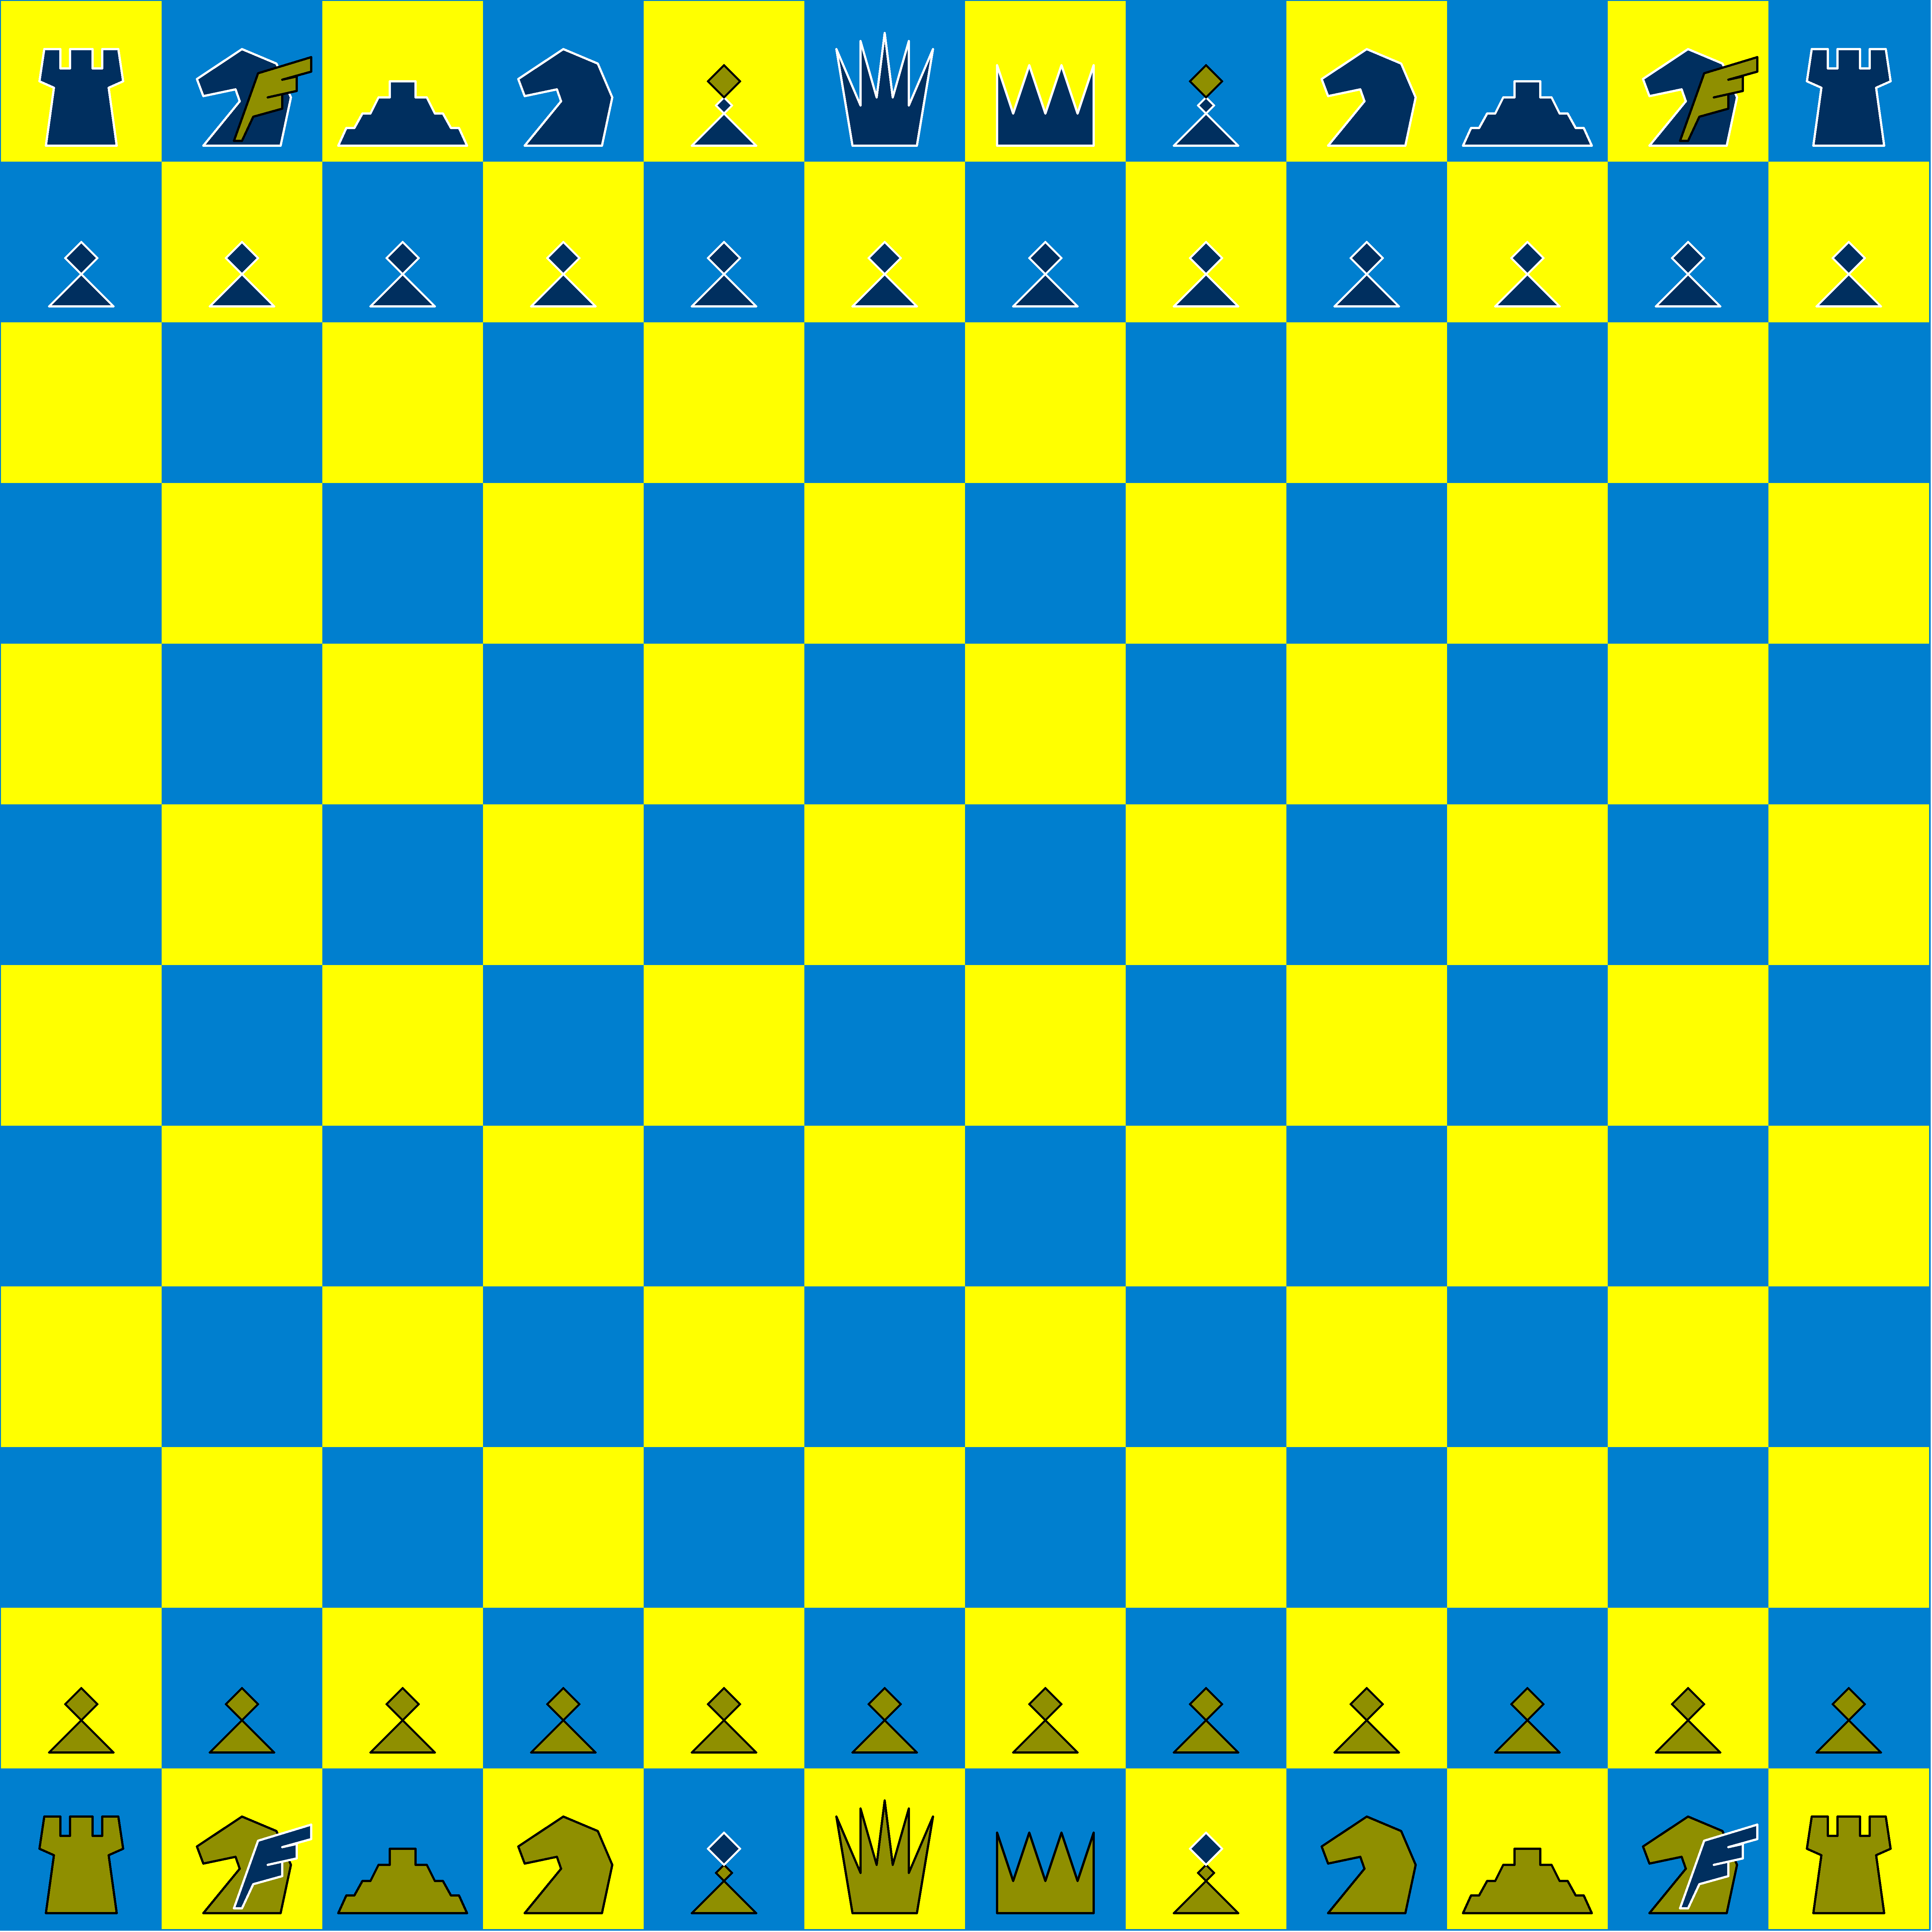
\includegraphics[width=1.0\textwidth, keepaspectratio=true]{../gfx/boards/06_mayan_ascendancy.png}
\caption{Mayan Ascendancy board}
\label{fig:mayan_ascendancy}
% \centering
\end{figure}

\clearpage
% -------------------------------------------- Mayan Ascendancy chapter

% Age of Aquarius chapter ---------------------------------------------
\chapter*{Age of Aquarius}
\addcontentsline{toc}{chapter}{Age of Aquarius}

\begin{flushright}
\parbox{0.8\textwidth}{
\emph{The greatest difficulty with the world is not its ability to produce, but the unwillingness to share. \\
\hspace*{\fill}{\textperiodcentered \textperiodcentered \textperiodcentered \hspace*{0.2em} Roy L. Smith} } }
\end{flushright}

Age of Aquarius is chess variant which is played on 14 x 14 board,
with light yellow and light green fields and light tan-gold and
dark green pieces. In algebraic notation, columns are enumerated
from 'a' to 'n', and rows are enumerated from '1' to '14'. A new
piece is introduced, Unicorn.

\clearpage

\section*{Unicorn}
\addcontentsline{toc}{section}{Unicorn}

\noindent
\begin{wrapfigure}{l}{0.4\textwidth}
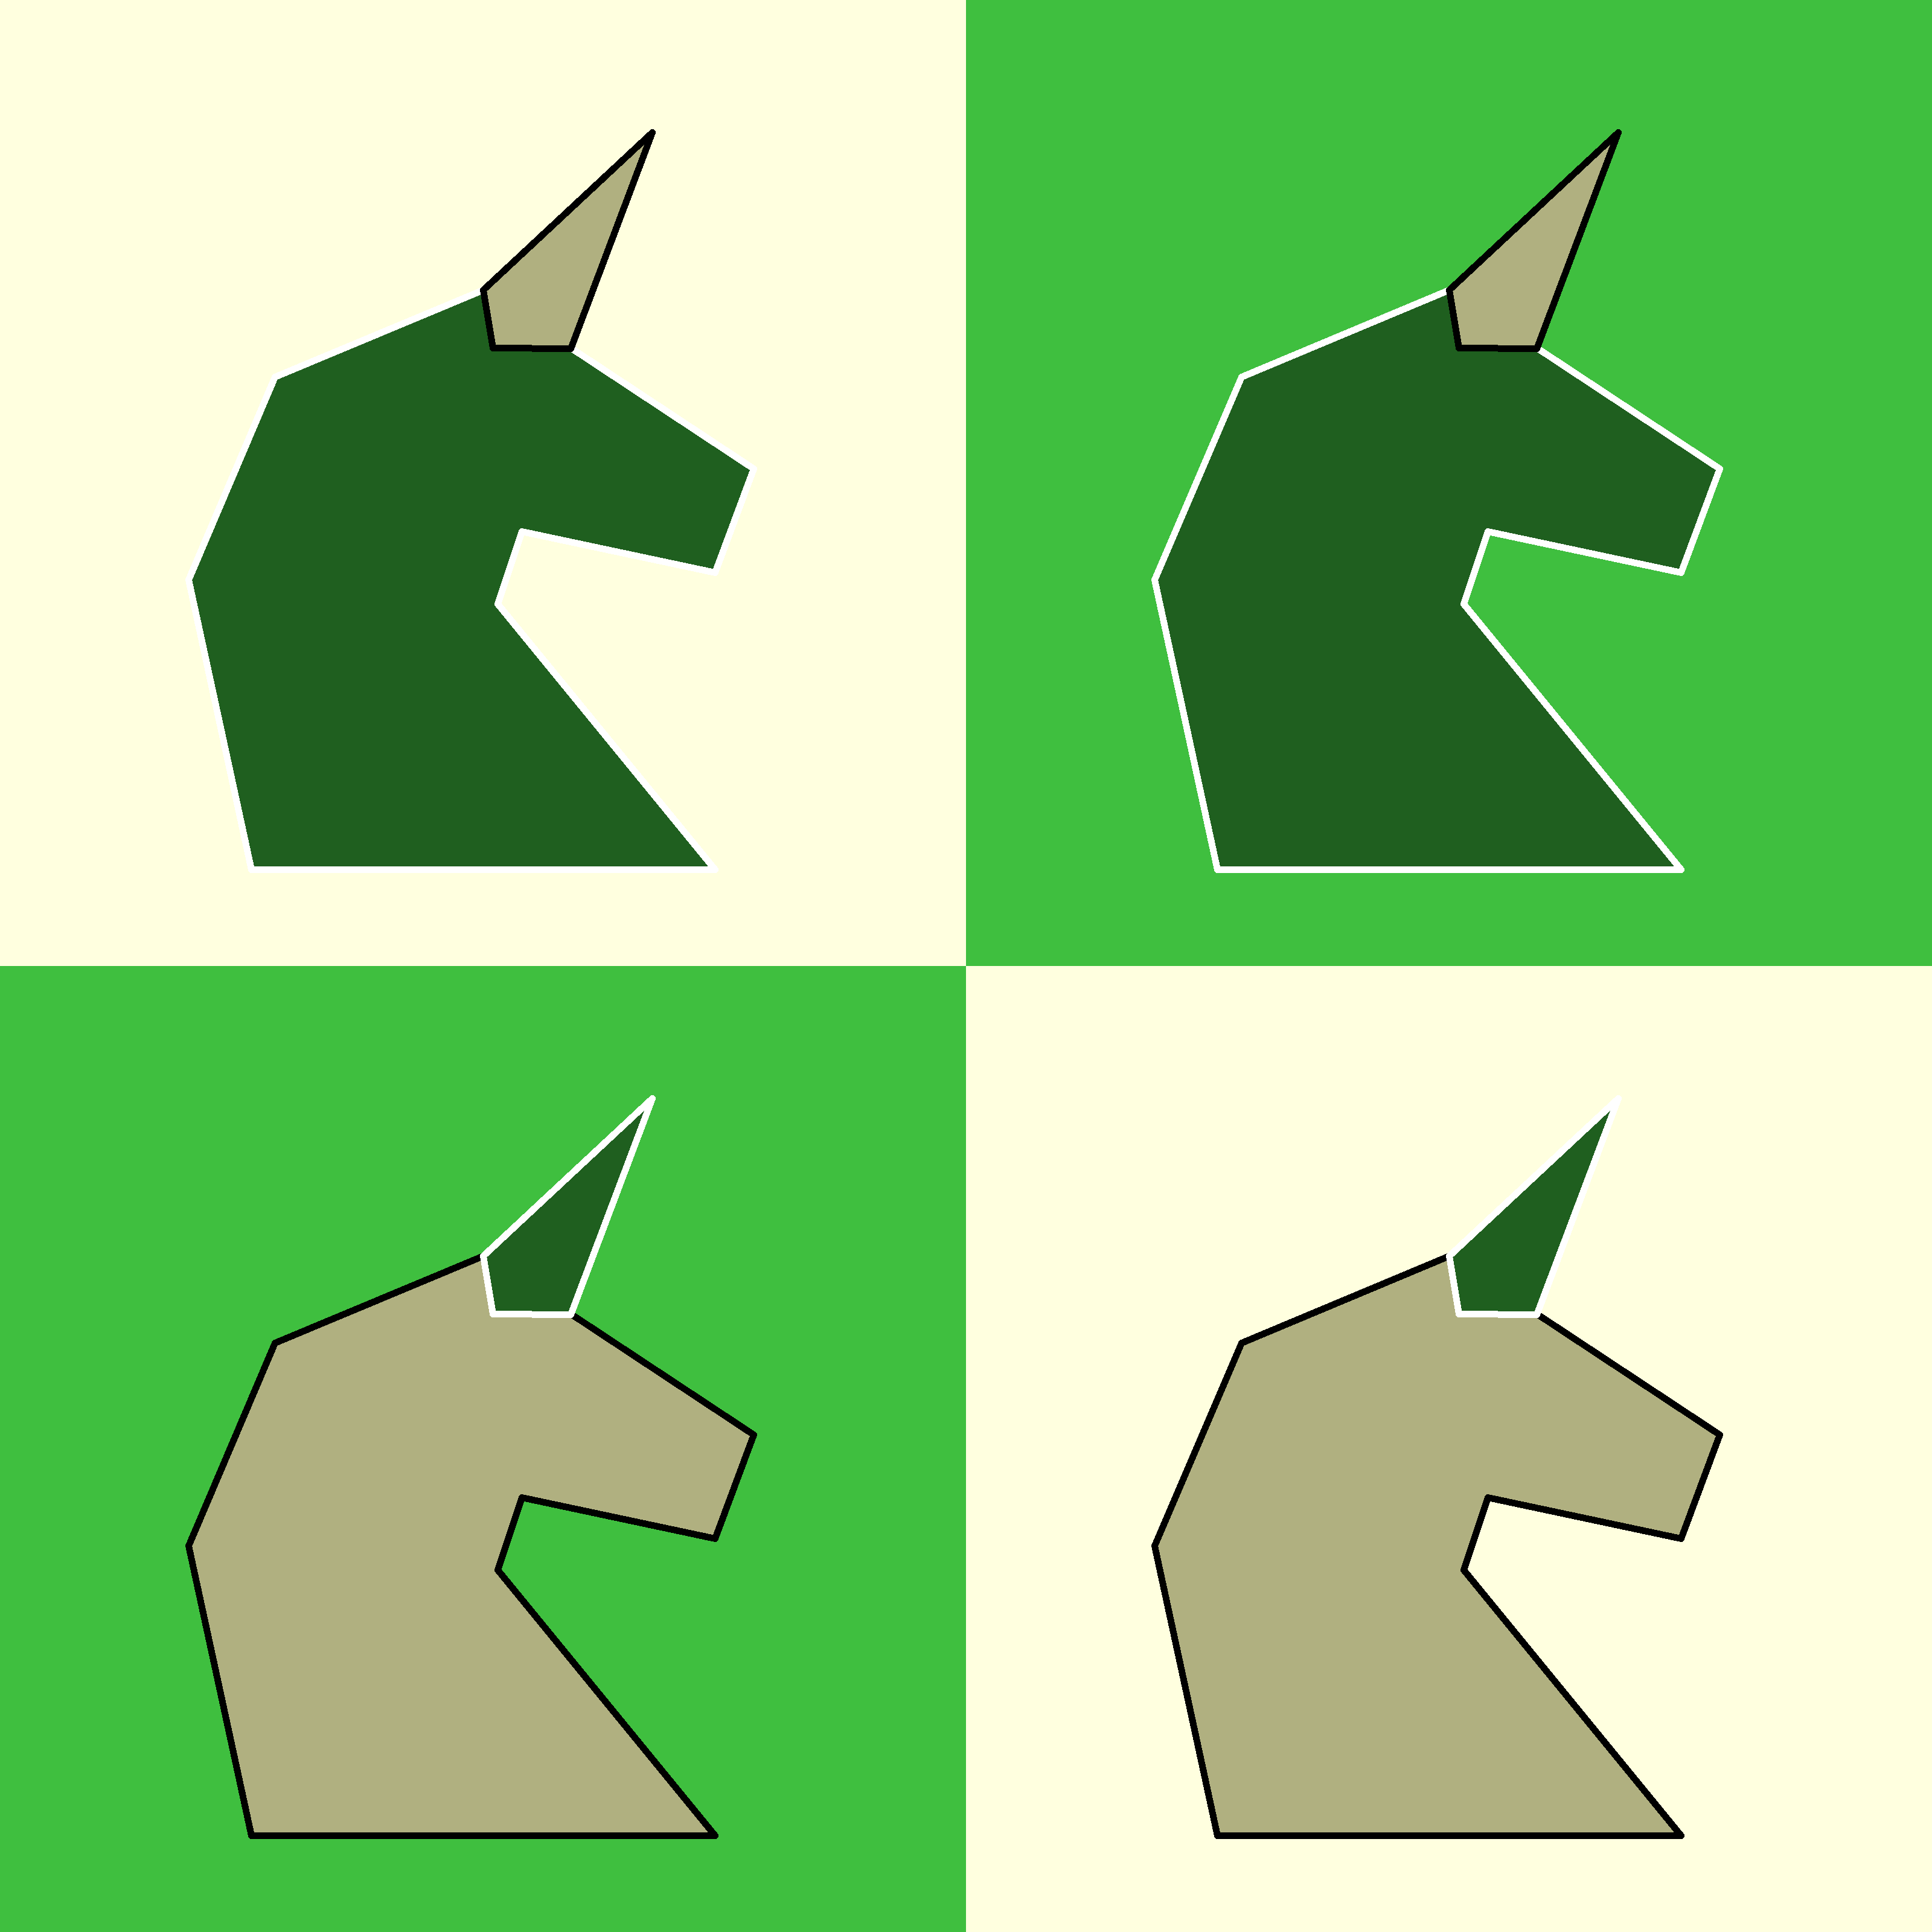
\includegraphics[width=0.4\textwidth, keepaspectratio=true]{../gfx/pieces/09_unicorn.png}
\caption{Unicorn}
\label{fig:unicorn}
% % \centering
\end{wrapfigure}

\clearpage

\section*{Initial setup}
\addcontentsline{toc}{section}{Initial setup}

Initial setup for Light player is (mirrored for Dark one):
\texttt{PPPPPPPPPPPPPP \\
        RGAUNBQKBNUAGR}, \\
or more conveniently, as seen in this image:

\noindent
% \begin{figure}[t]
\begin{figure}[h]
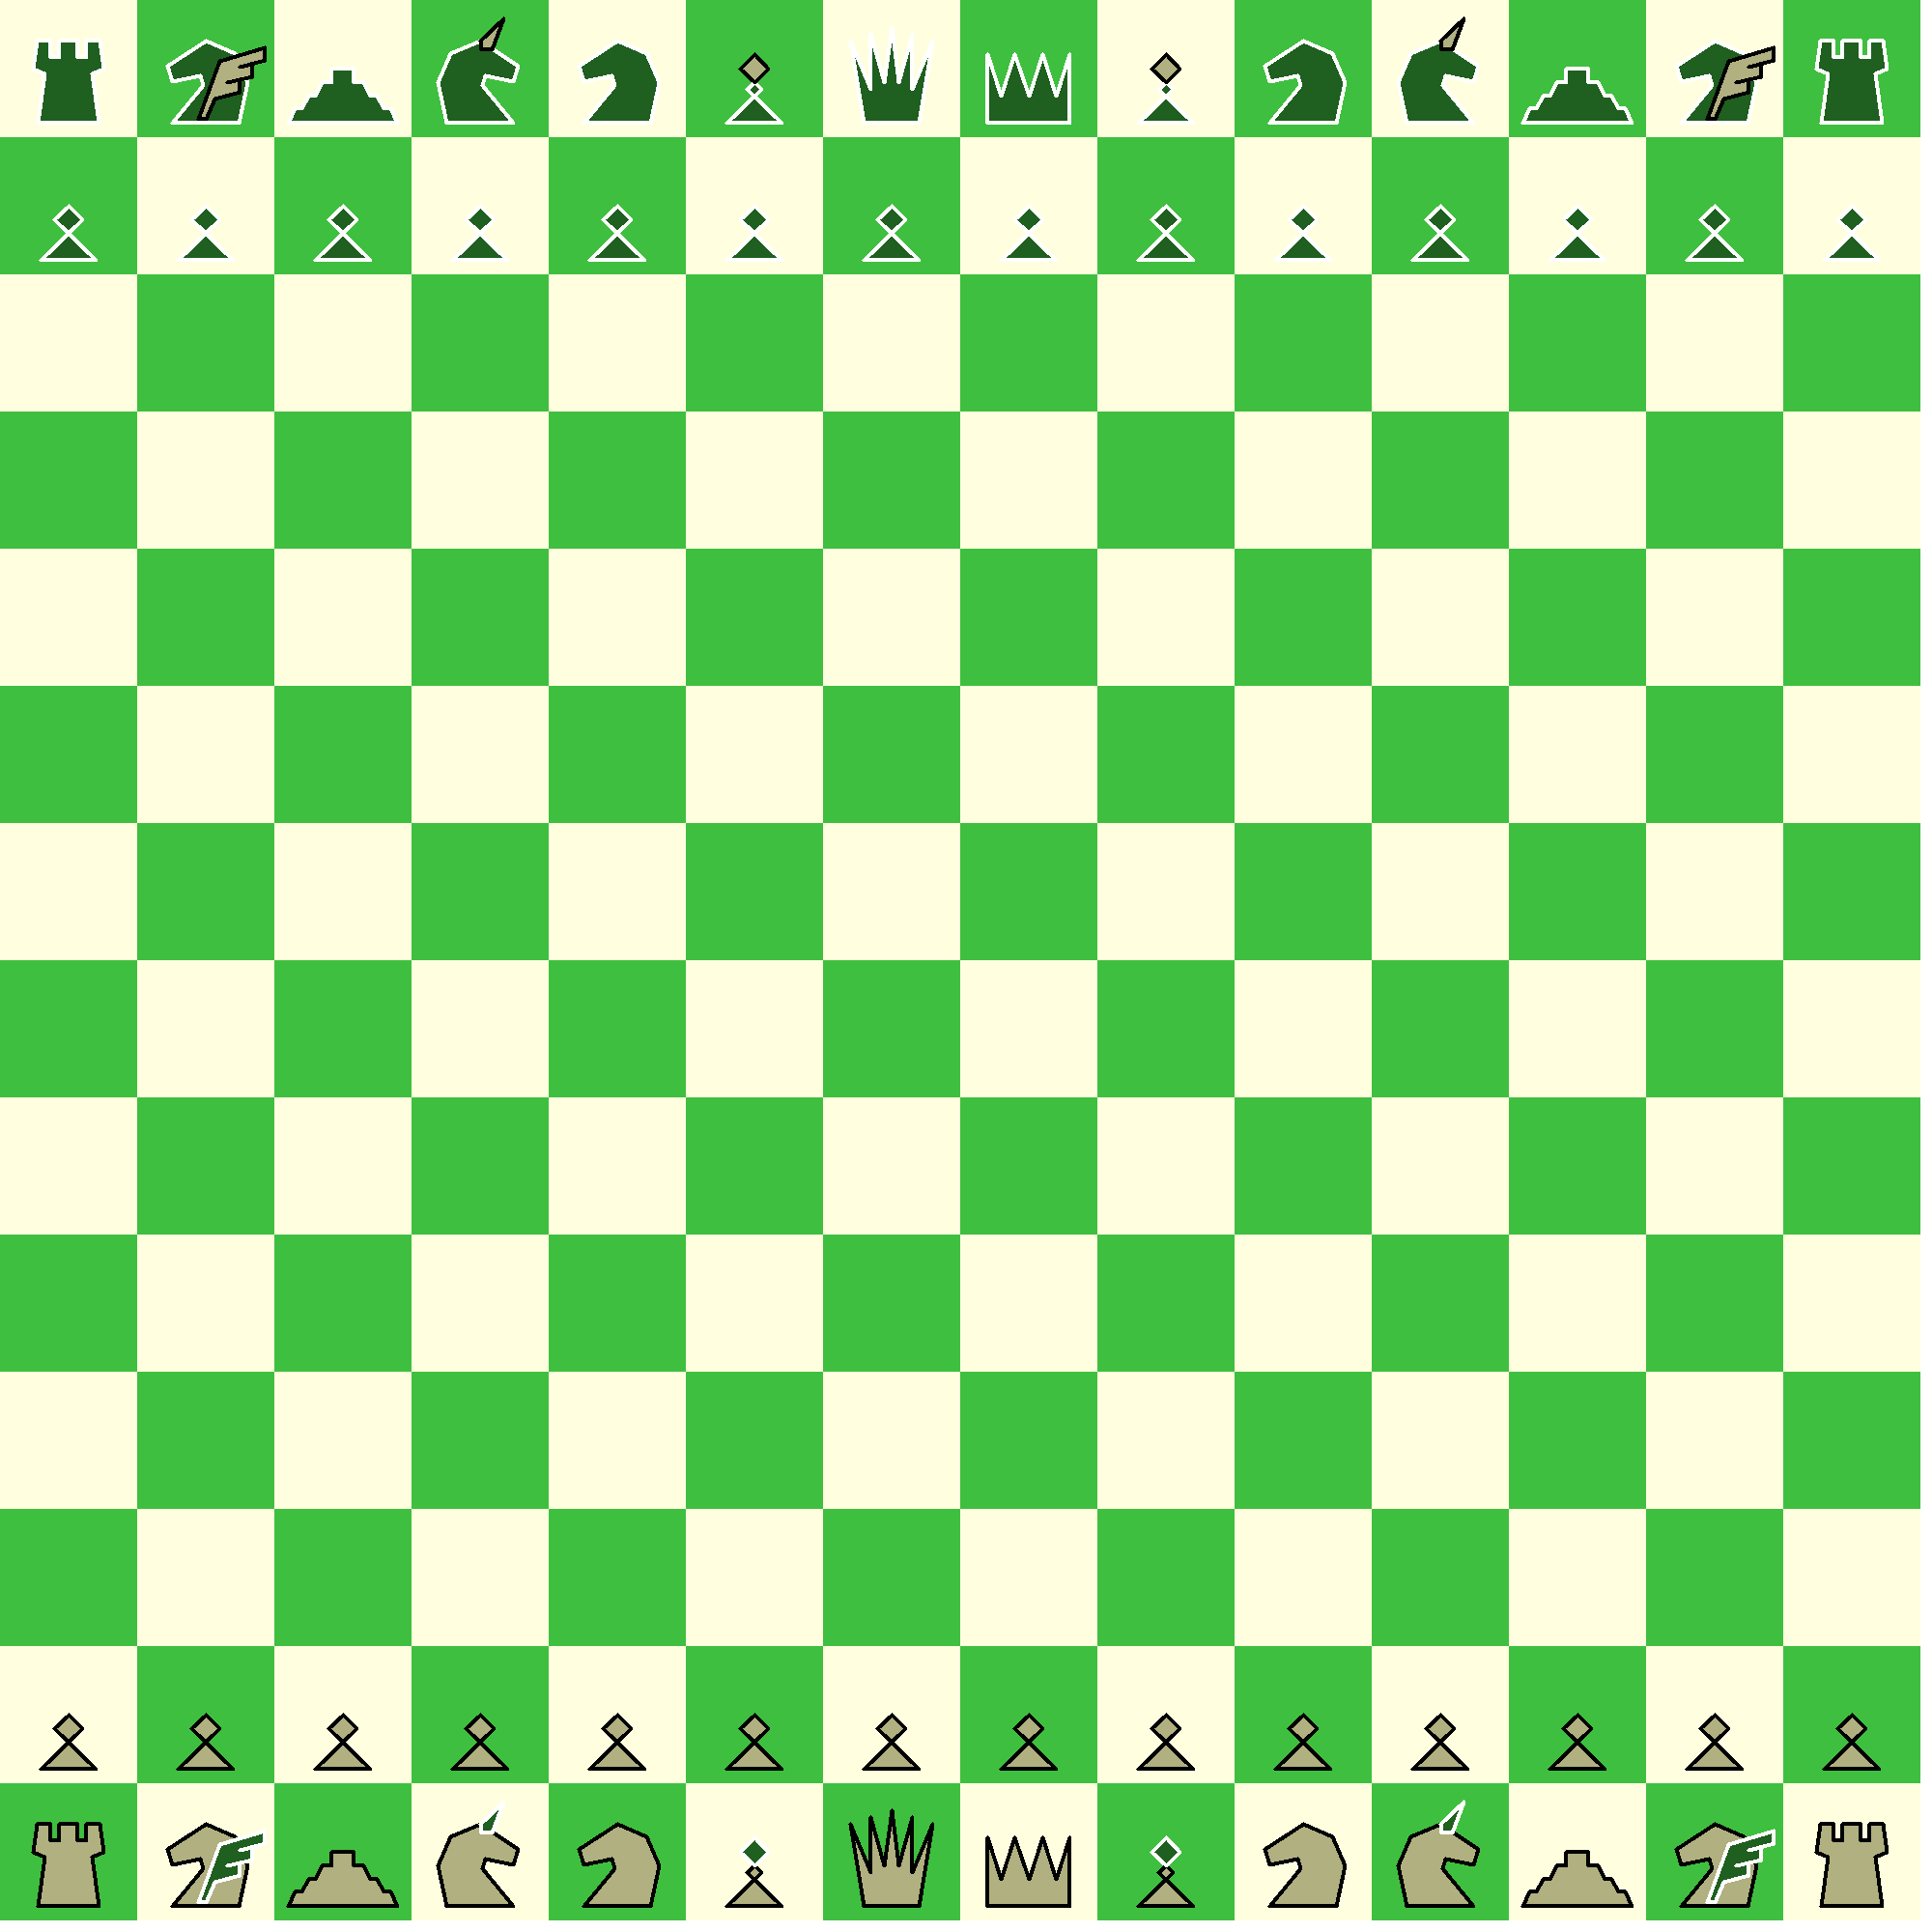
\includegraphics[width=1.0\textwidth, keepaspectratio=true]{../gfx/boards/08_age_of_aquarius.png}
\caption{Age of Aquarius board}
\label{fig:age_of_aquarius}
% \centering
\end{figure}

\clearpage
% --------------------------------------------- Age of Aquarius chapter

% Miranda's veil chapter ----------------------------------------------
\chapter*{Miranda's veil}
\addcontentsline{toc}{chapter}{Miranda's veil}

\begin{flushright}
\parbox{0.8\textwidth}{
\emph{Under all that we think, lives all we believe, like the ultimate veil of our spirits. \\
\hspace*{\fill}{\textperiodcentered \textperiodcentered \textperiodcentered \hspace*{0.2em} Antonio Machado} } }
\end{flushright}

Miranda's veil is chess variant which is played on 16 x 16 board,
with light yellow and dark violet fields and light pink and dark
gray-violet pieces. In algebraic notation, columns are enumerated
from 'a' to 'p', and rows are enumerated from '1' to '16'. A new
piece is introduced, Wave.

\clearpage

\section*{Wave}
\addcontentsline{toc}{section}{Wave}

\noindent
\begin{wrapfigure}{l}{0.4\textwidth}

\includegraphics[width=0.4\textwidth, keepaspectratio=true]{../gfx/pieces/10_wave.png}
\caption{Wave}
\label{fig:wave}
% % \centering
\end{wrapfigure}

\clearpage

\section*{Initial setup}
\addcontentsline{toc}{section}{Initial setup}

Initial setup for Light player is (mirrored for Dark one):
\texttt{PPPPPPPPPPPPPPPP \\
        RGAUWNBQKBNWUAGR}, \\
or more conveniently, as seen in this image:

\noindent
% \begin{figure}[t]
\begin{figure}[h]
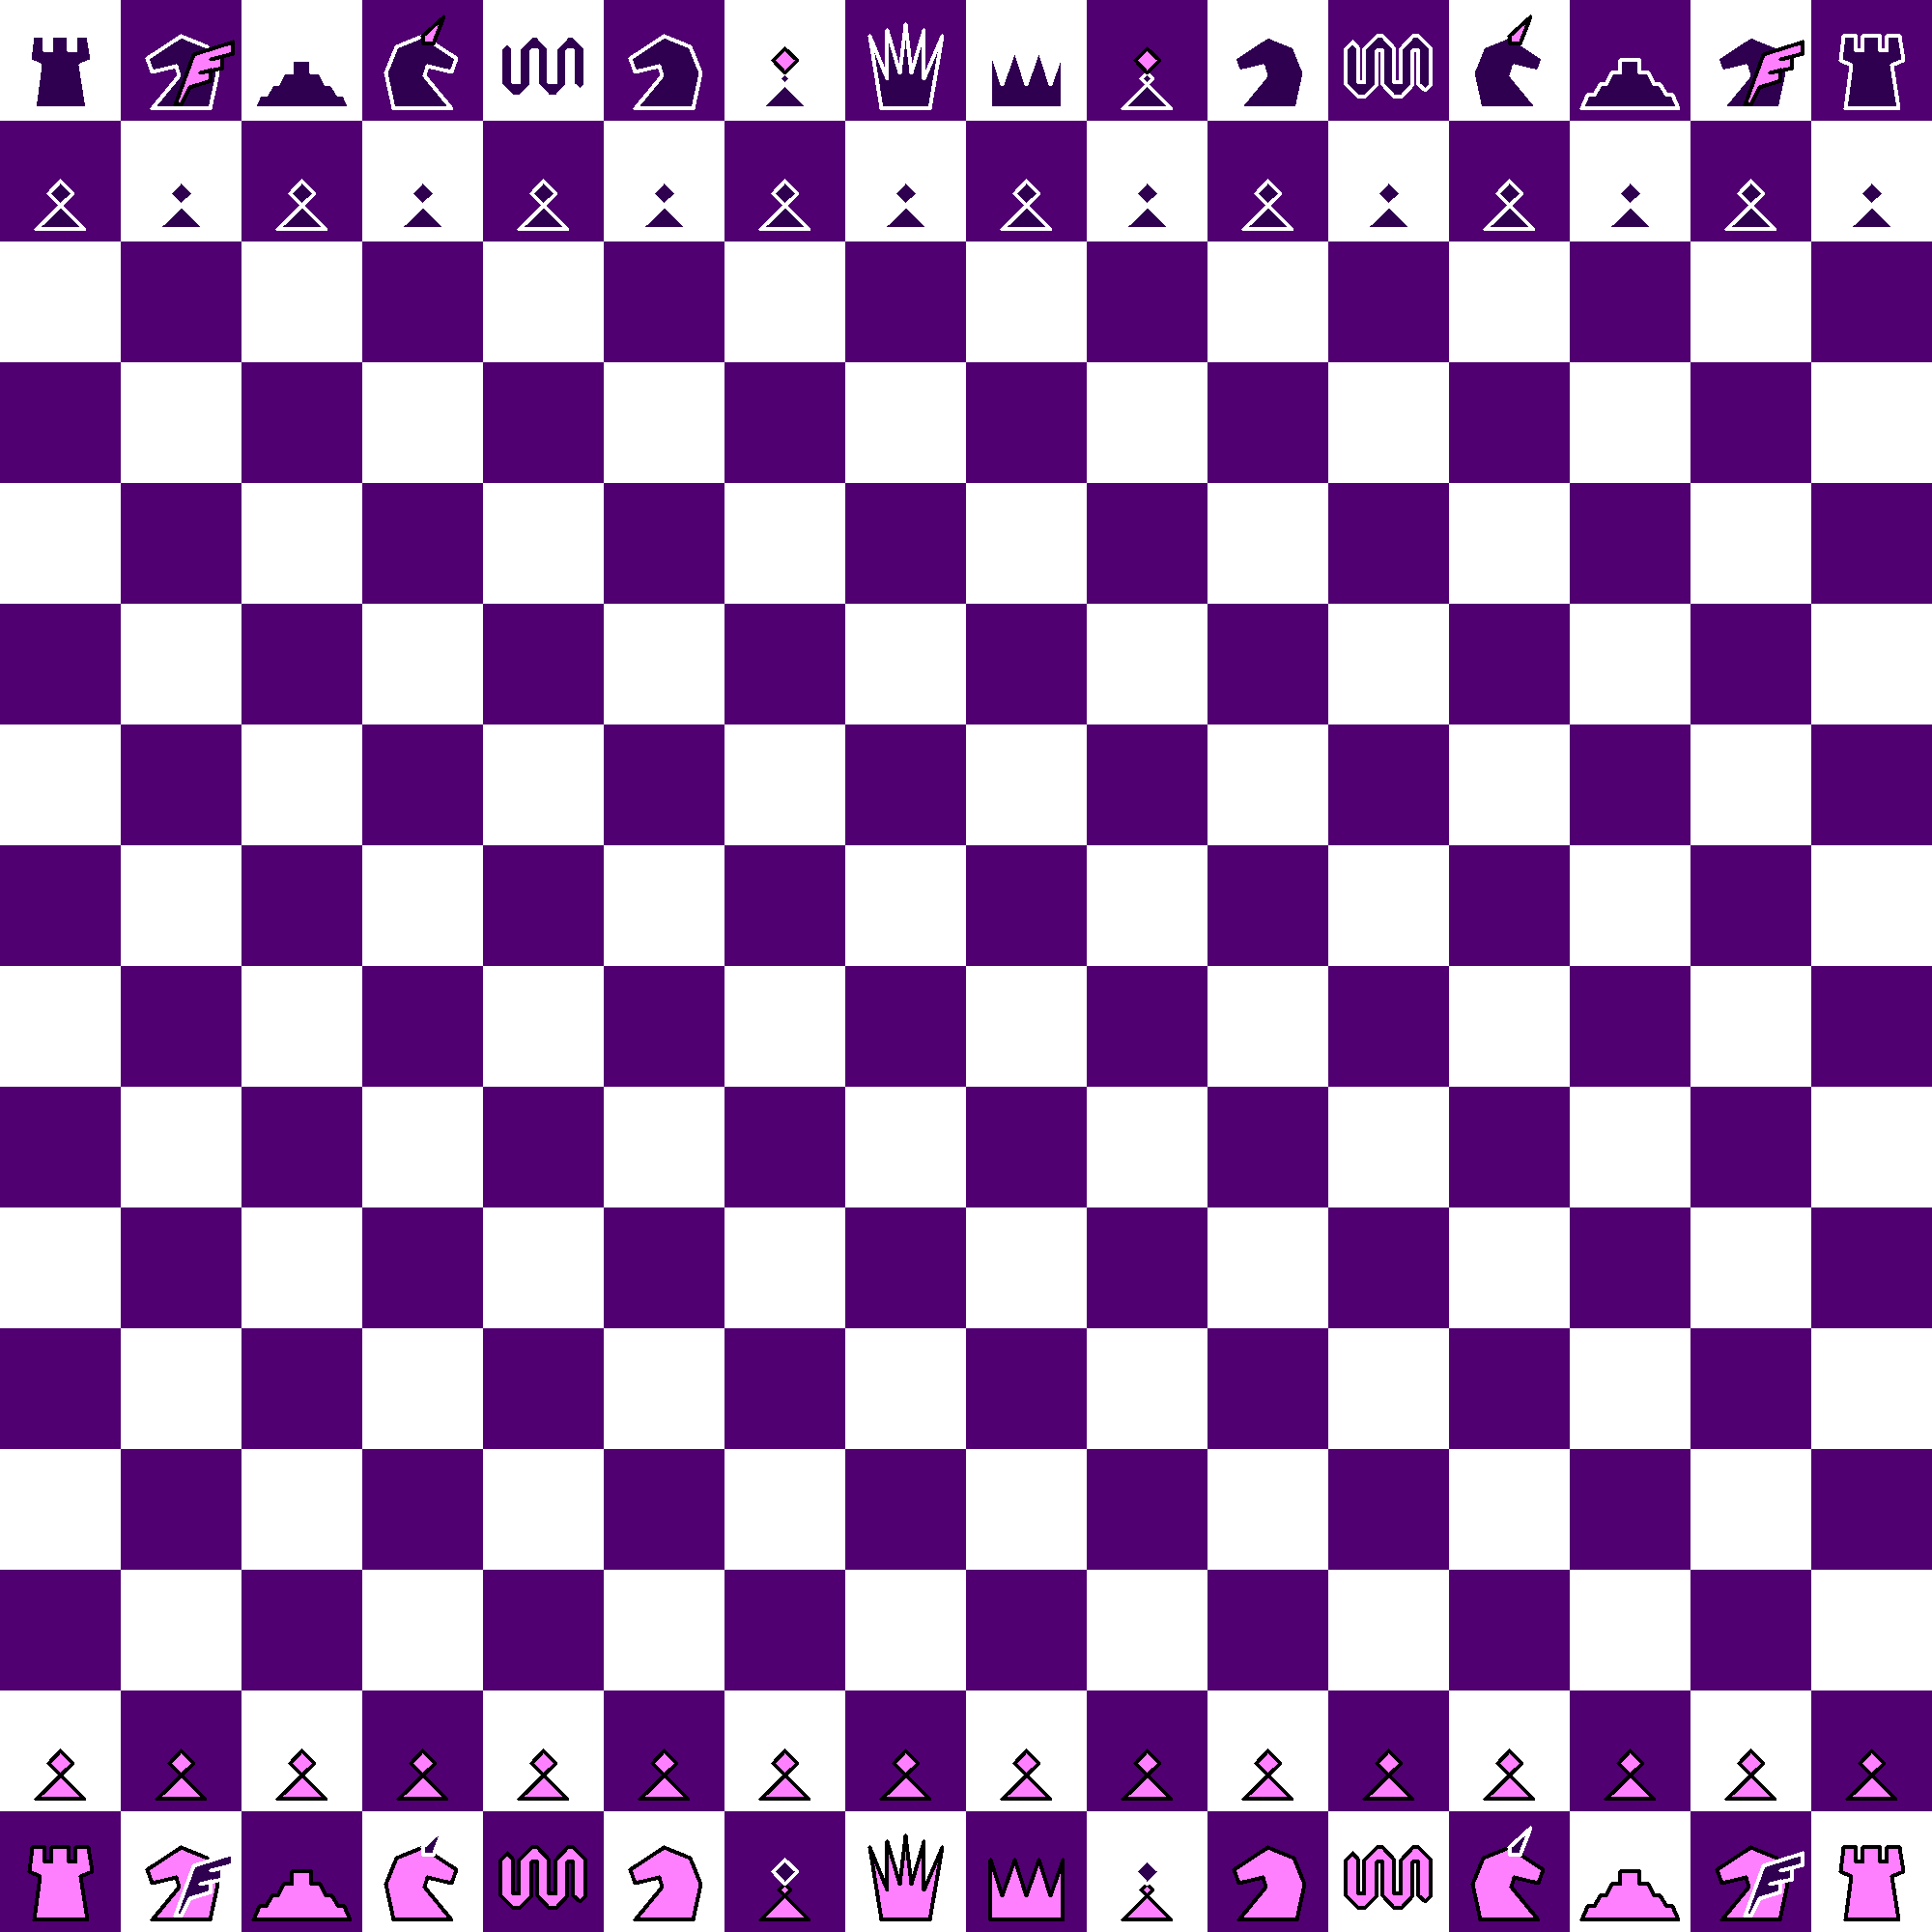
\includegraphics[width=1.0\textwidth, keepaspectratio=true]{../gfx/boards/10_miranda_s_veil.png}
\caption{Miranda's veil board}
\label{fig:miranda_s_veil}
% \centering
\end{figure}

\clearpage
% ---------------------------------------------- Miranda's veil chapter

% Nineteen chapter ----------------------------------------------------
\chapter*{Nineteen}
\addcontentsline{toc}{chapter}{Nineteen}

\begin{flushright}
\parbox{0.8\textwidth}{
\emph{The truth is at the beginning of anything and its end are alike touching. \\
\hspace*{\fill}{\textperiodcentered \textperiodcentered \textperiodcentered \hspace*{0.2em} Yoshida Kenko} } }
\end{flushright}

Nineteen is chess variant which is played on 18 x 18 board, with
light gold-yellow and white fields and gold-yellow and dark gray
pieces. In algebraic notation, columns are enumerated from 'a' to 'r',
and rows are enumerated from '1' to '18'. A new piece is introduced,
Star.

\clearpage

\section*{Star}
\addcontentsline{toc}{section}{Star}

\noindent
\begin{wrapfigure}{l}{0.4\textwidth}
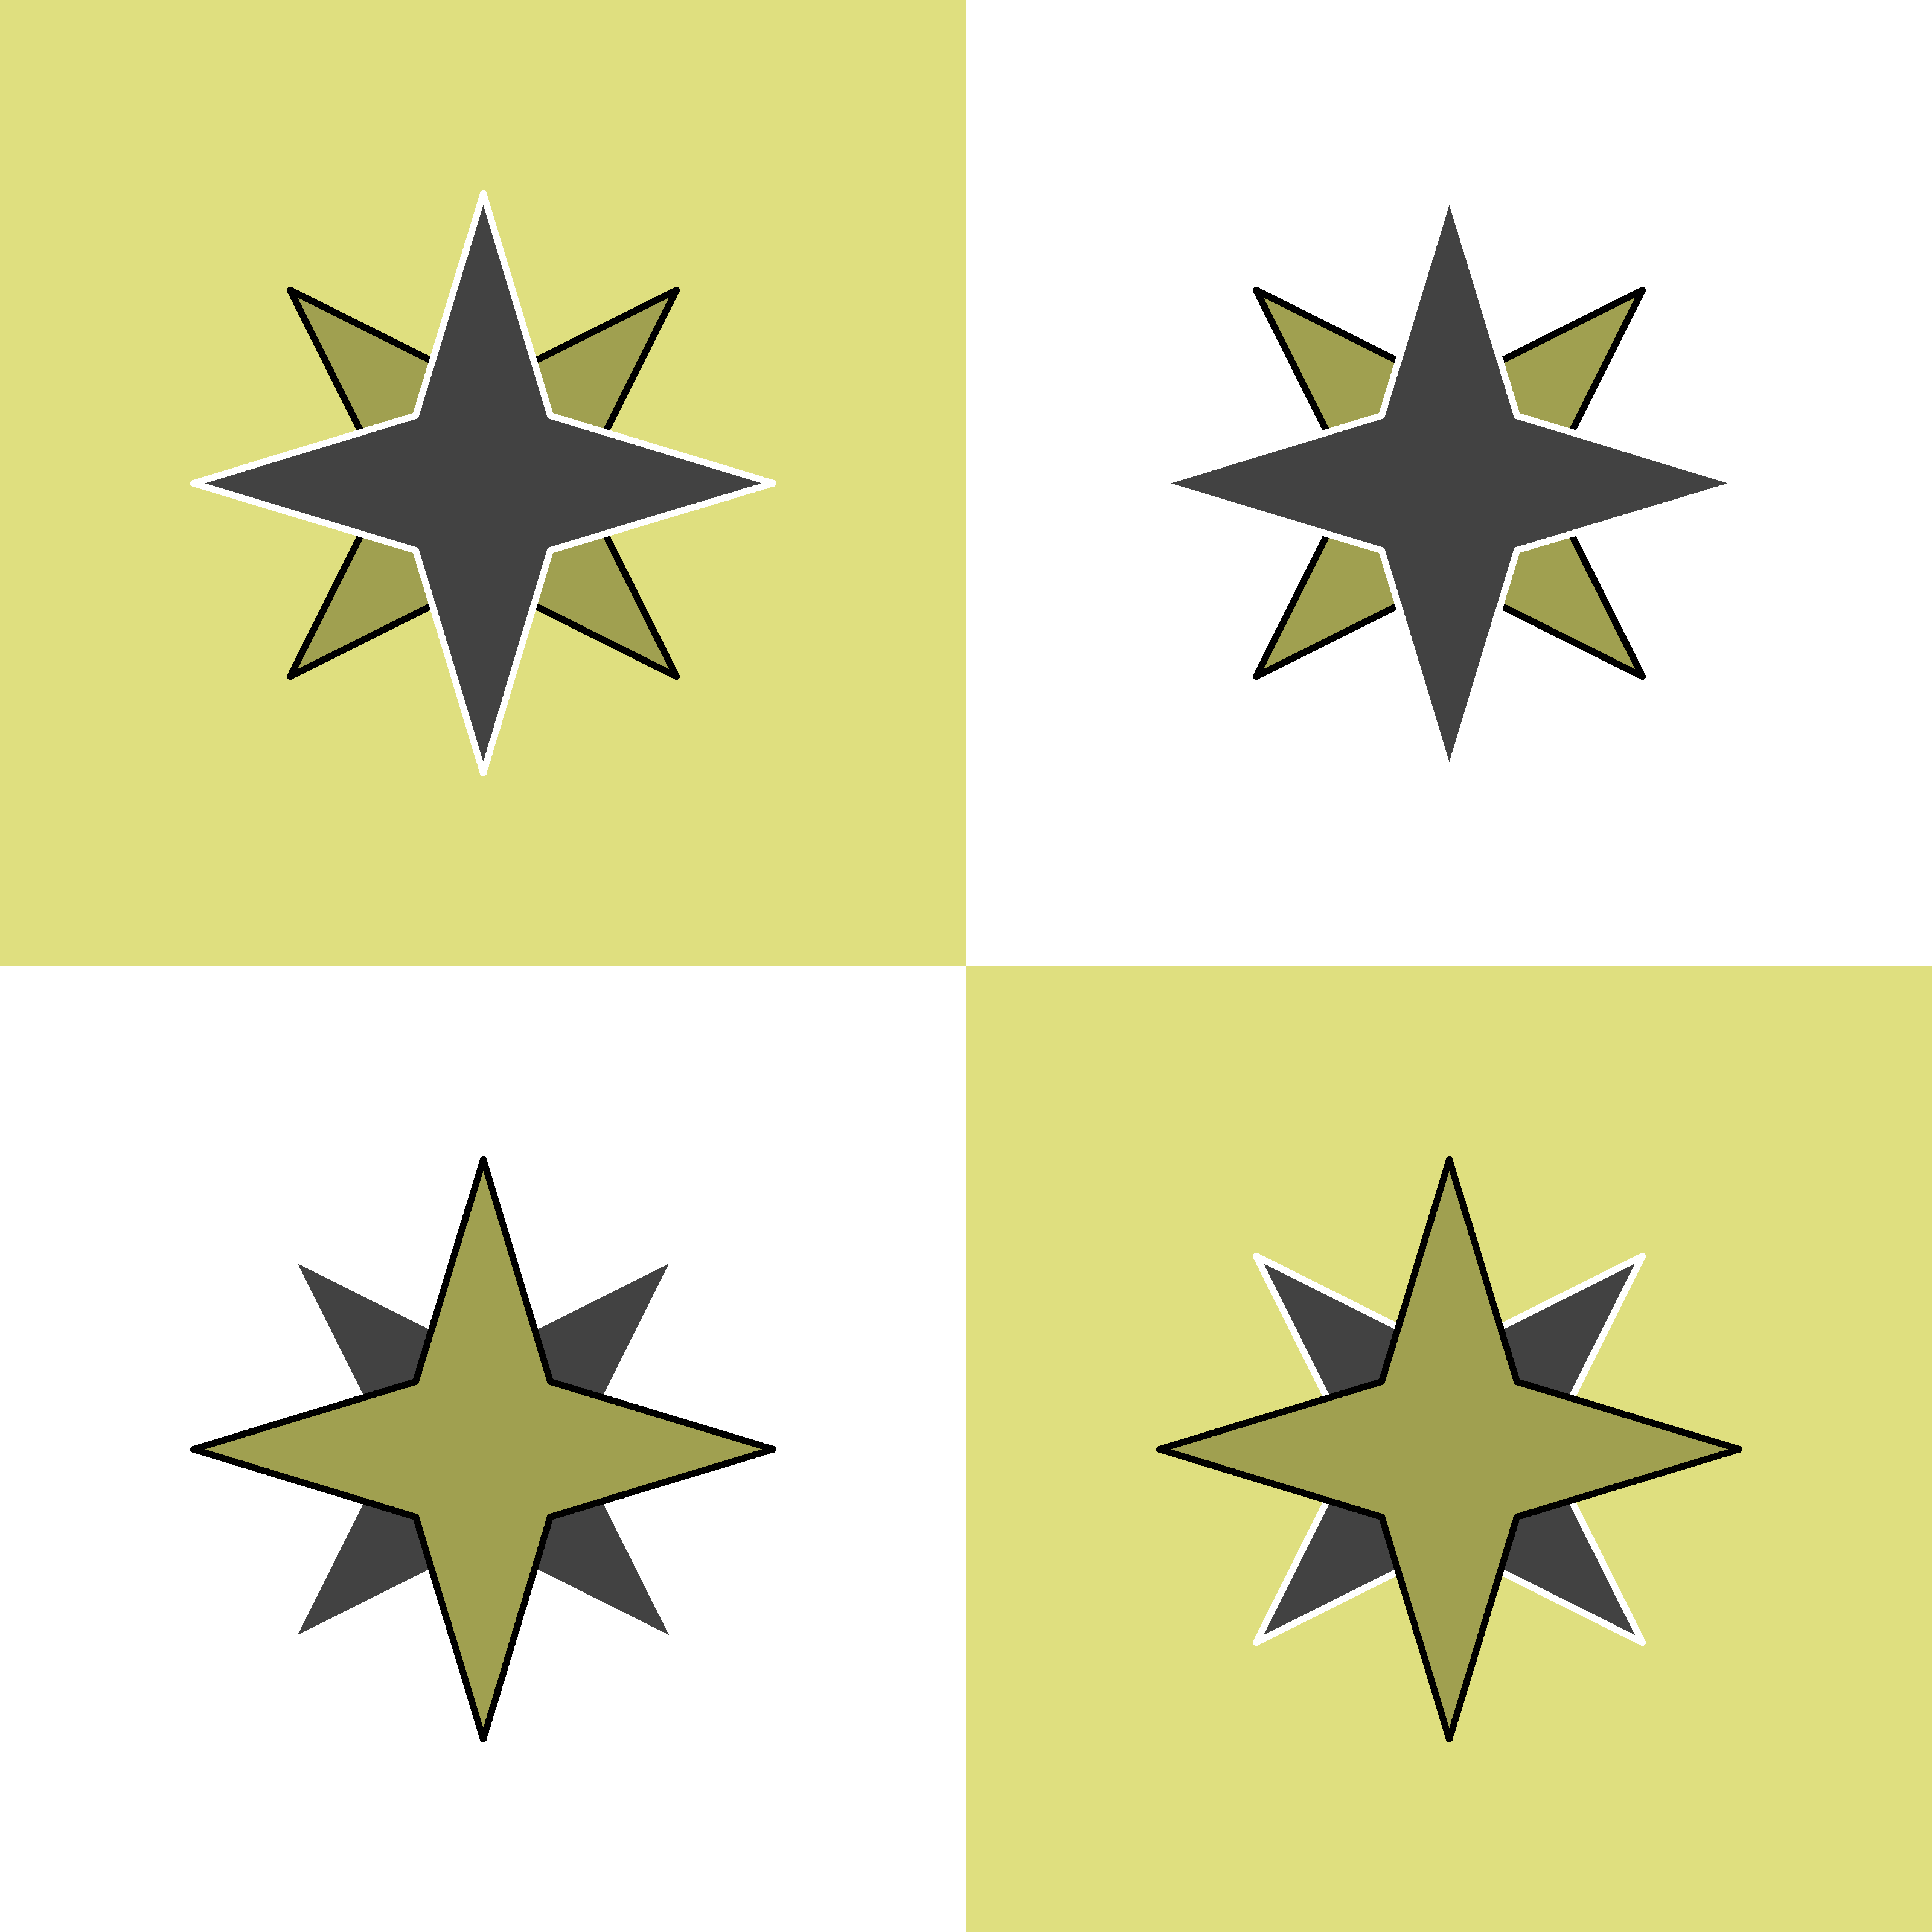
\includegraphics[width=0.4\textwidth, keepaspectratio=true]{../gfx/pieces/11_star.png}
\caption{Star}
\label{fig:star}
% % \centering
\end{wrapfigure}

\clearpage

\section*{Initial setup}
\addcontentsline{toc}{section}{Initial setup}

Initial setup for Light player is (mirrored for Dark one):
\texttt{PPPPPPPPPPPPPPPPPP \\
        TRGAUWNBQKBNWUAGRT}, \\
or more conveniently, as seen in this image:

\noindent
% \begin{figure}[t]
\begin{figure}[h]
\includegraphics[width=1.0\textwidth, keepaspectratio=true]{../gfx/boards/12_nineteen.png}
\caption{Nineteen board}
\label{fig:nineteen}
% \centering
\end{figure}

\clearpage
% ---------------------------------------------------- Nineteen chapter

% Hemera's Dawn chapter -----------------------------------------------
\chapter*{Hemera's Dawn}
\addcontentsline{toc}{chapter}{Hemera's Dawn}

\begin{flushright}
\parbox{0.8\textwidth}{
\emph{Then assuredly the world was made, not in time, but simultaneously with time. \\
\hspace*{\fill}{\textperiodcentered \textperiodcentered \textperiodcentered \hspace*{0.2em} St. Augustine} } }
\end{flushright}

Hemera's Dawn is chess variant which is played on 20 x 20 board, with
darkish red-brown and gray fields and bright red and dark gray pieces.
In algebraic notation, columns are enumerated from 'a' to 't', and rows
are enumerated from '1' to '20'. A new piece is introduced, Centaur.

\clearpage

\section*{Centaur}
\addcontentsline{toc}{section}{Centaur}

\noindent
\begin{wrapfigure}{l}{0.4\textwidth}
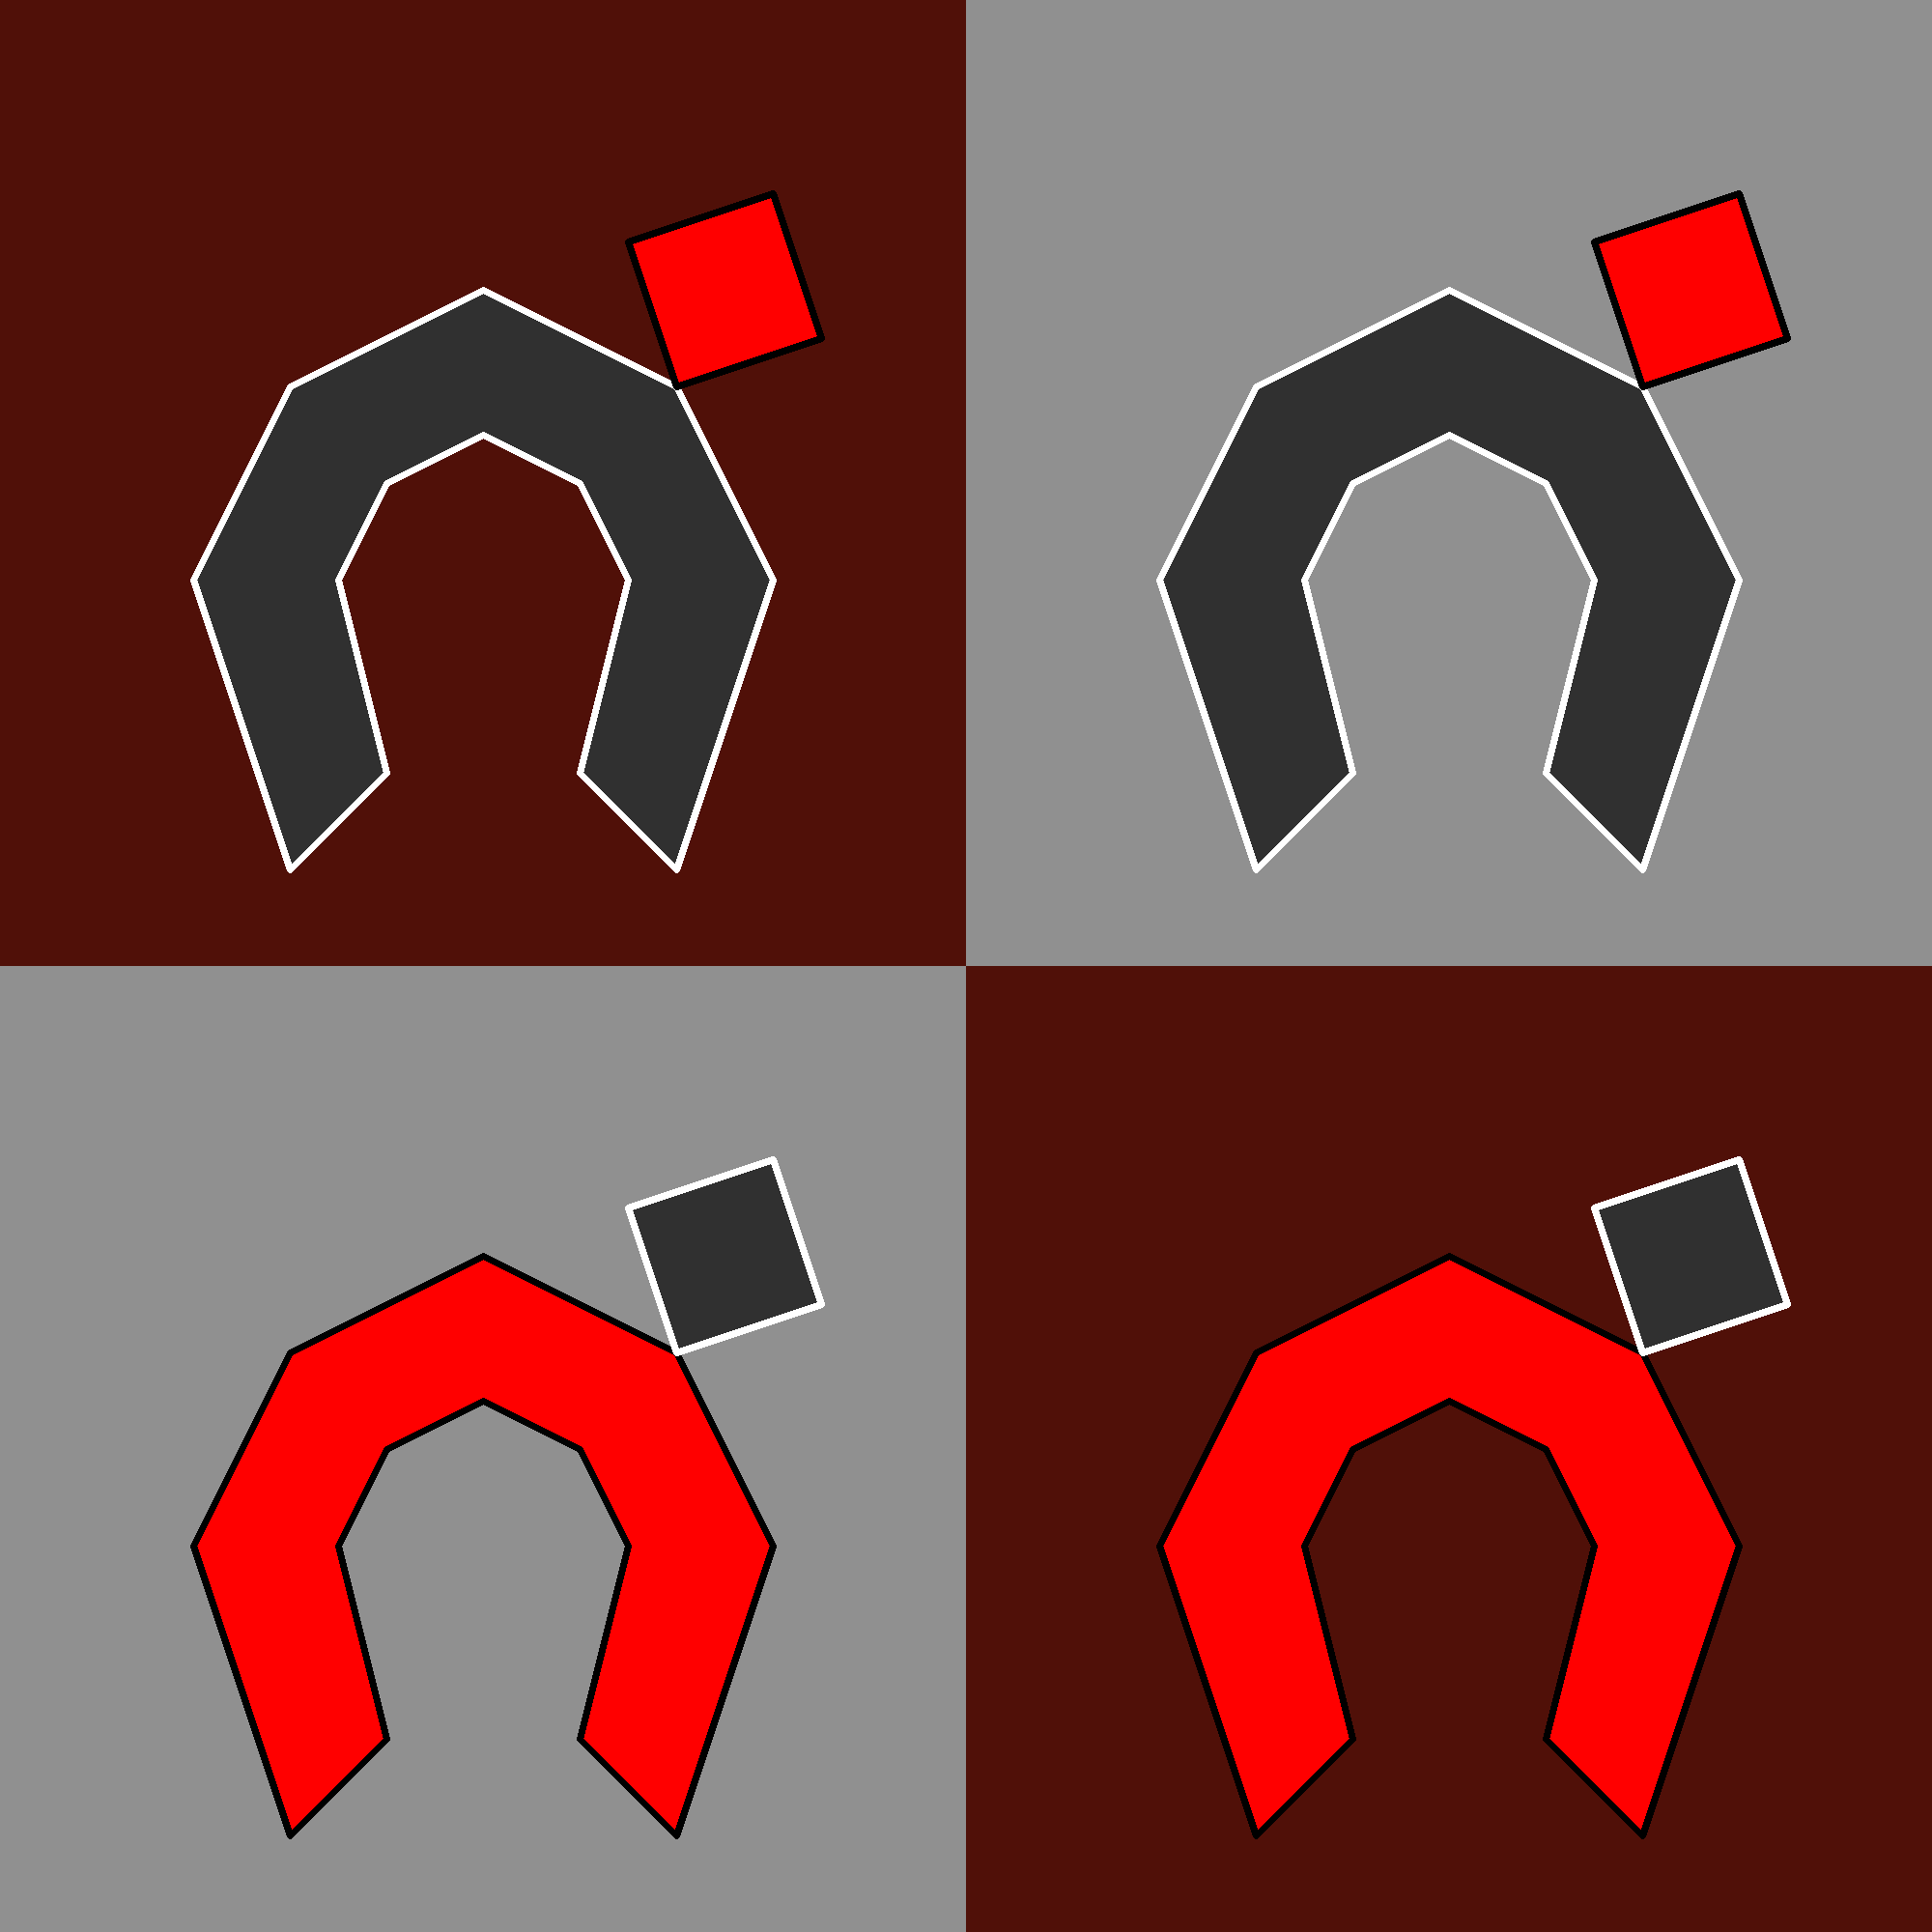
\includegraphics[width=0.4\textwidth, keepaspectratio=true]{../gfx/pieces/12_centaur.png}
\caption{Centaur}
\label{fig:centaur}
% % \centering
\end{wrapfigure}

\clearpage

\section*{Initial setup}
\addcontentsline{toc}{section}{Initial setup}

Initial setup for Light player is (mirrored for Dark one):
\texttt{PPPPPPPPPPPPPPPPPPPP \\
        TRGAUWCNBQKBNCWUAGRT}, \\
or more conveniently, as seen in this image:

\noindent
% \begin{figure}[t]
\begin{figure}[h]
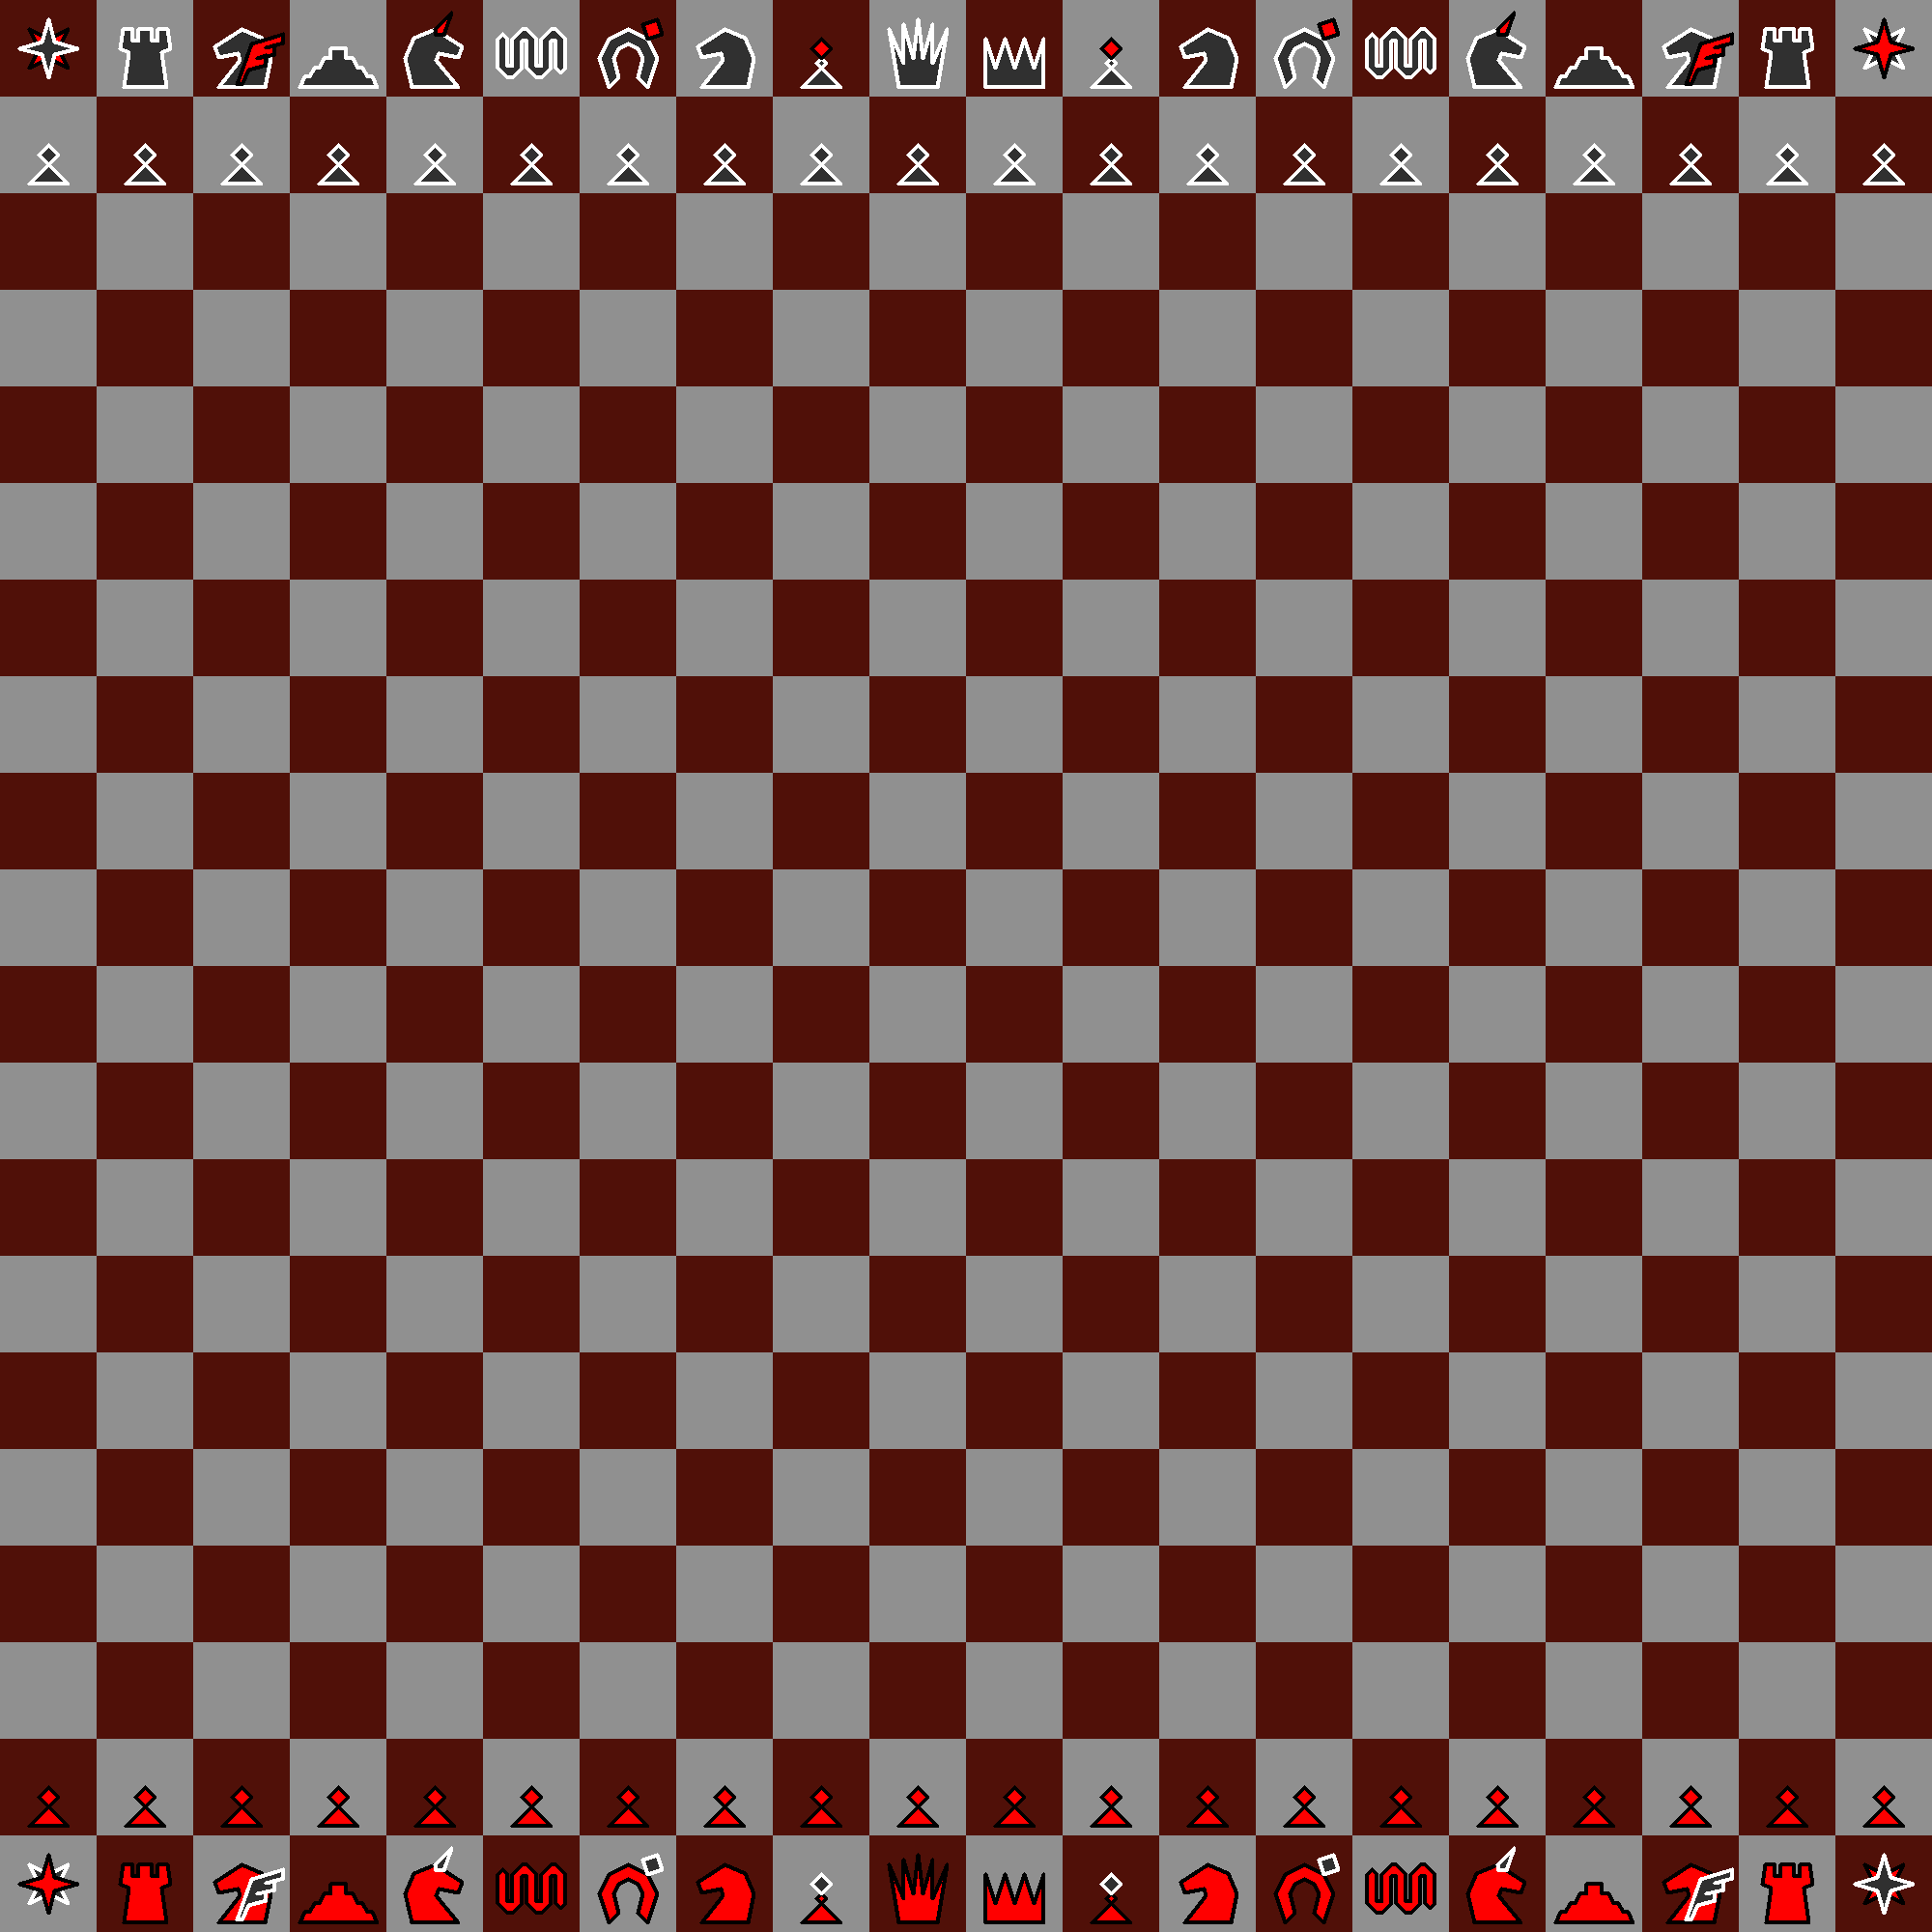
\includegraphics[width=1.0\textwidth, keepaspectratio=true]{../gfx/boards/14_hemera_s_dawn.png}
\caption{Hemera's Dawn board}
\label{fig:hemera_s_dawn}
% \centering
\end{figure}

\clearpage
% ----------------------------------------------- Hemera's Dawn chapter

% Tamoanchan Revisited chapter ----------------------------------------
\chapter*{Tamoanchan Revisited}
\addcontentsline{toc}{chapter}{Tamoanchan Revisited}

\begin{flushright}
\parbox{0.6\textwidth}{
\emph{I dream, therefore I exist. \\
\hspace*{\fill}{\textperiodcentered \textperiodcentered \textperiodcentered \hspace*{0.2em} August Strindberg} } }
\end{flushright}

Tamoanchan Revisited is chess variant which is played on 22 x 22 board,
with bright cyan and blue fields and light green and dark blue pieces.
In algebraic notation, columns are enumerated from 'a' to 'v', and rows
are enumerated from '1' to '22'. A new piece is introduced, Serpent.

\clearpage

\section*{Serpent}
\addcontentsline{toc}{section}{Serpent}

\noindent
\begin{wrapfigure}{l}{0.4\textwidth}
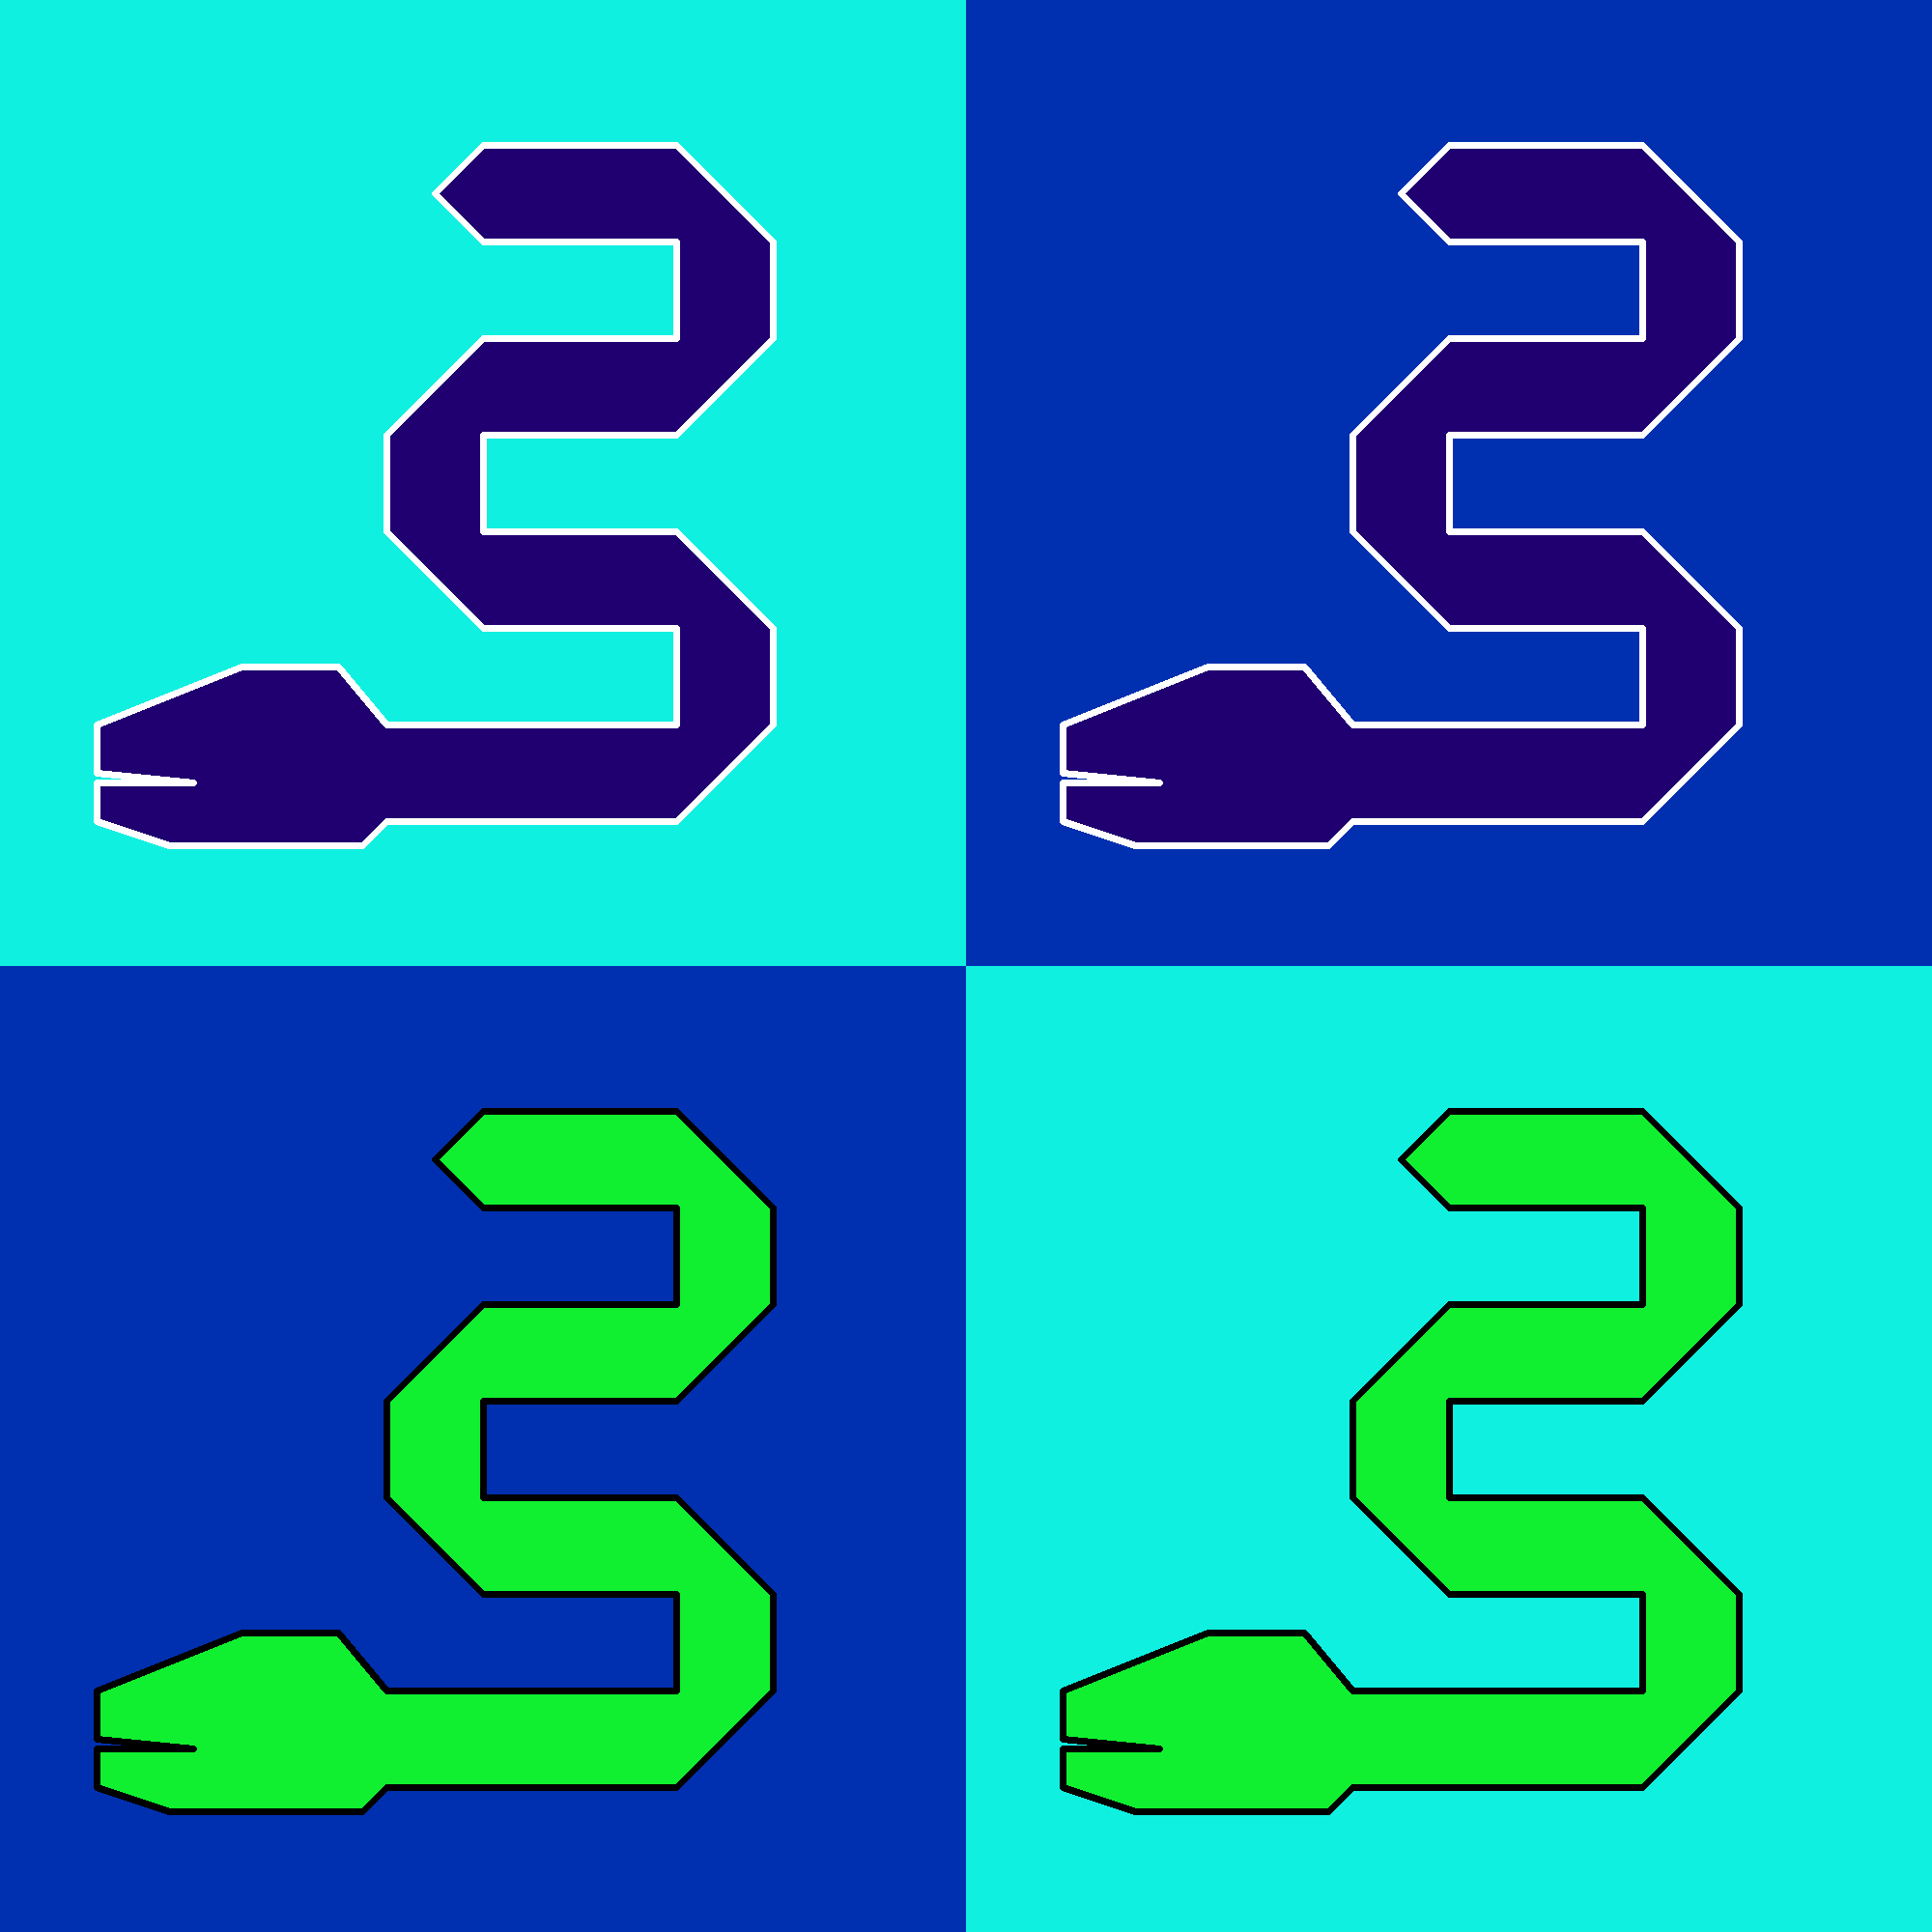
\includegraphics[width=0.4\textwidth, keepaspectratio=true]{../gfx/pieces/13_serpent.png}
\caption{Serpent}
\label{fig:serpent}
% % \centering
\end{wrapfigure}

\clearpage

\section*{Initial setup}
\addcontentsline{toc}{section}{Initial setup}

Initial setup for Light player is (mirrored for Dark one):
\texttt{PPPPPPPPPPPPPPPPPPPPPP \\
        TRGAUWCSNBQKBNSCWUAGRT}, \\
or more conveniently, as seen in this image:

\noindent
% \begin{figure}[t]
\begin{figure}[h]
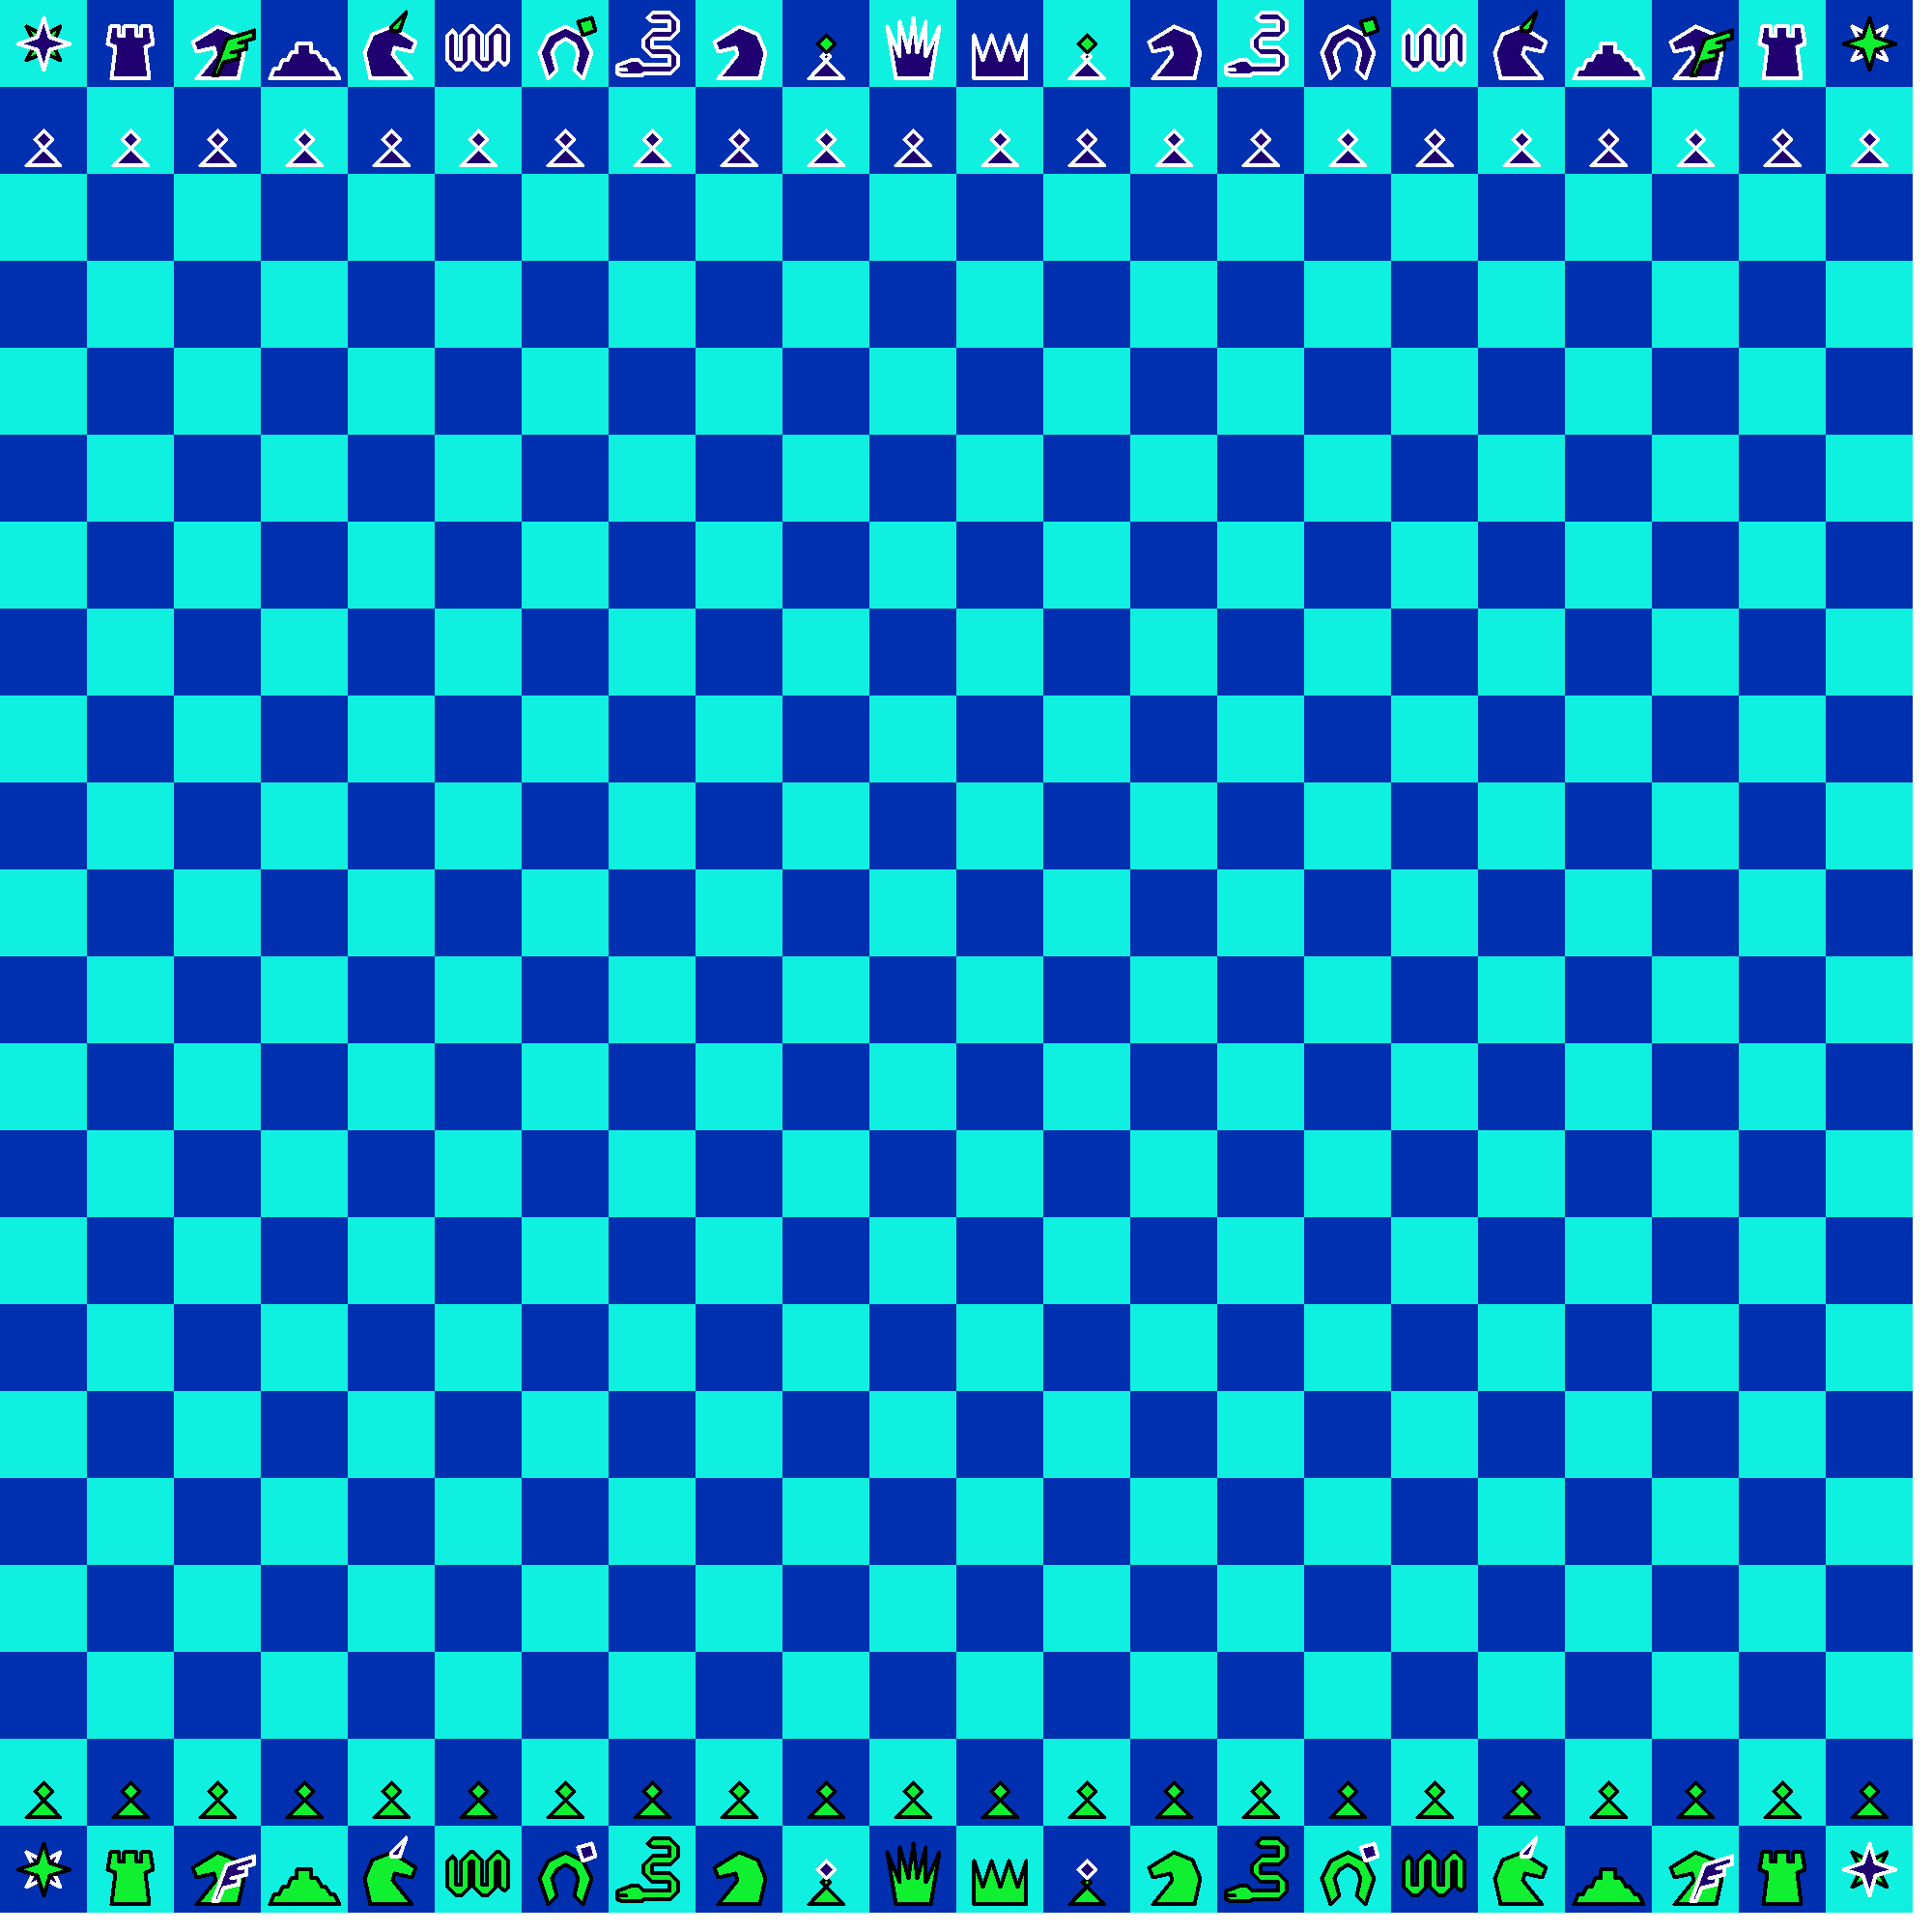
\includegraphics[width=1.0\textwidth, keepaspectratio=true]{../gfx/boards/16_tamoanchan_revisited.png}
\caption{Tamoanchan Revisited board}
\label{fig:tamoanchan_revisited}
% \centering
\end{figure}

\clearpage
% ---------------------------------------- Tamoanchan Revisited chapter

% Conquest of Tlalocan chapter ----------------------------------------
\chapter*{Conquest of Tlalocan}
\addcontentsline{toc}{chapter}{Conquest of Tlalocan}

\begin{flushright}
\parbox{0.8\textwidth}{
\emph{The human mind is inspired enough when it comes to inventing
horrors; it is when it tries to invent a Heaven that it shows itself
cloddish. \\
\hspace*{\fill}{\textperiodcentered \textperiodcentered \textperiodcentered \hspace*{0.2em} Evelyn Waugh} } }
\end{flushright}

Conquest of Tlalocan is chess variant which is played on 24 x 24 board,
with bright cyan and red fields and light green and dark red pieces.
In algebraic notation, columns are enumerated from 'a' to 'x', and rows
are enumerated from '1' to '24'. A new piece is introduced, Shaman.

\clearpage

\section*{Shaman}
\addcontentsline{toc}{section}{Shaman}

\noindent
\begin{wrapfigure}{l}{0.4\textwidth}
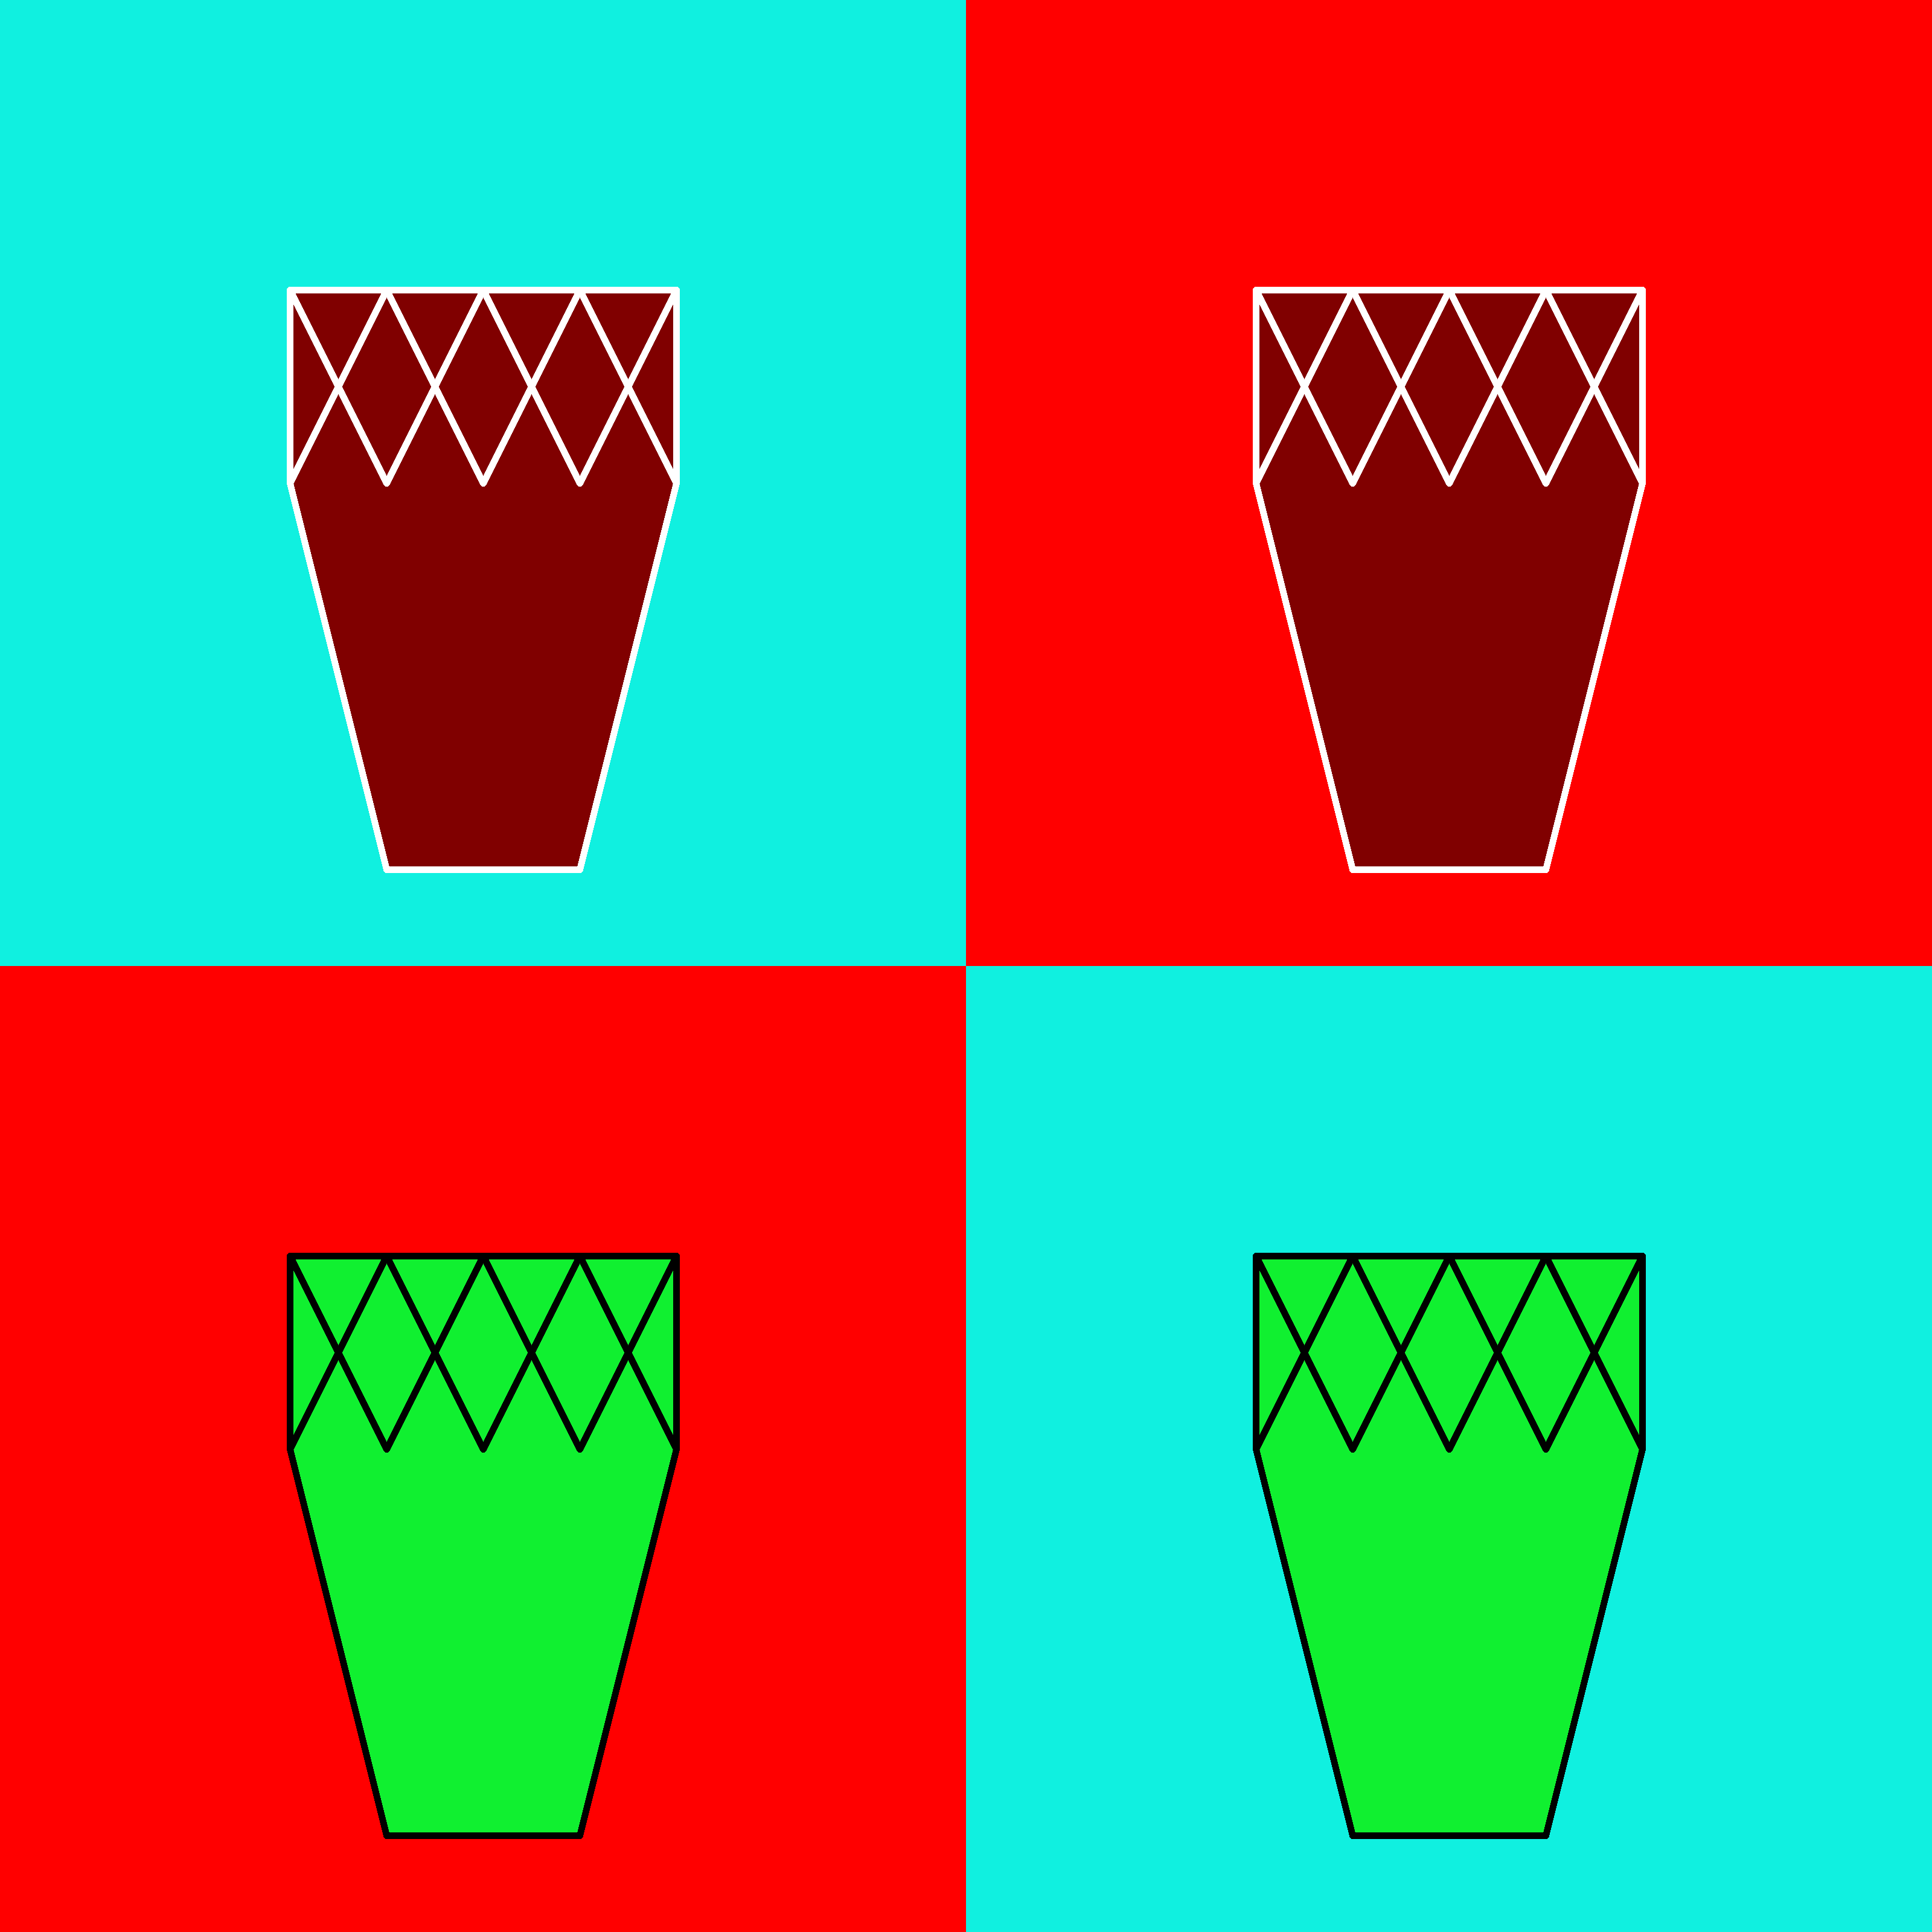
\includegraphics[width=0.4\textwidth, keepaspectratio=true]{../gfx/pieces/14_shaman.png}
\caption{Shaman}
\label{fig:shaman}
% % \centering
\end{wrapfigure}

\clearpage

\section*{Initial setup}
\addcontentsline{toc}{section}{Initial setup}

Initial setup for Light player is (mirrored for Dark one):
\texttt{PPPPPPPPPPPPPPPPPPPPPPPP \\
        TRGAHUWCSNBQKBNSCWUHAGRT}, \\
or more conveniently, as seen in this image:

\noindent
% \begin{figure}[t]
\begin{figure}[h]
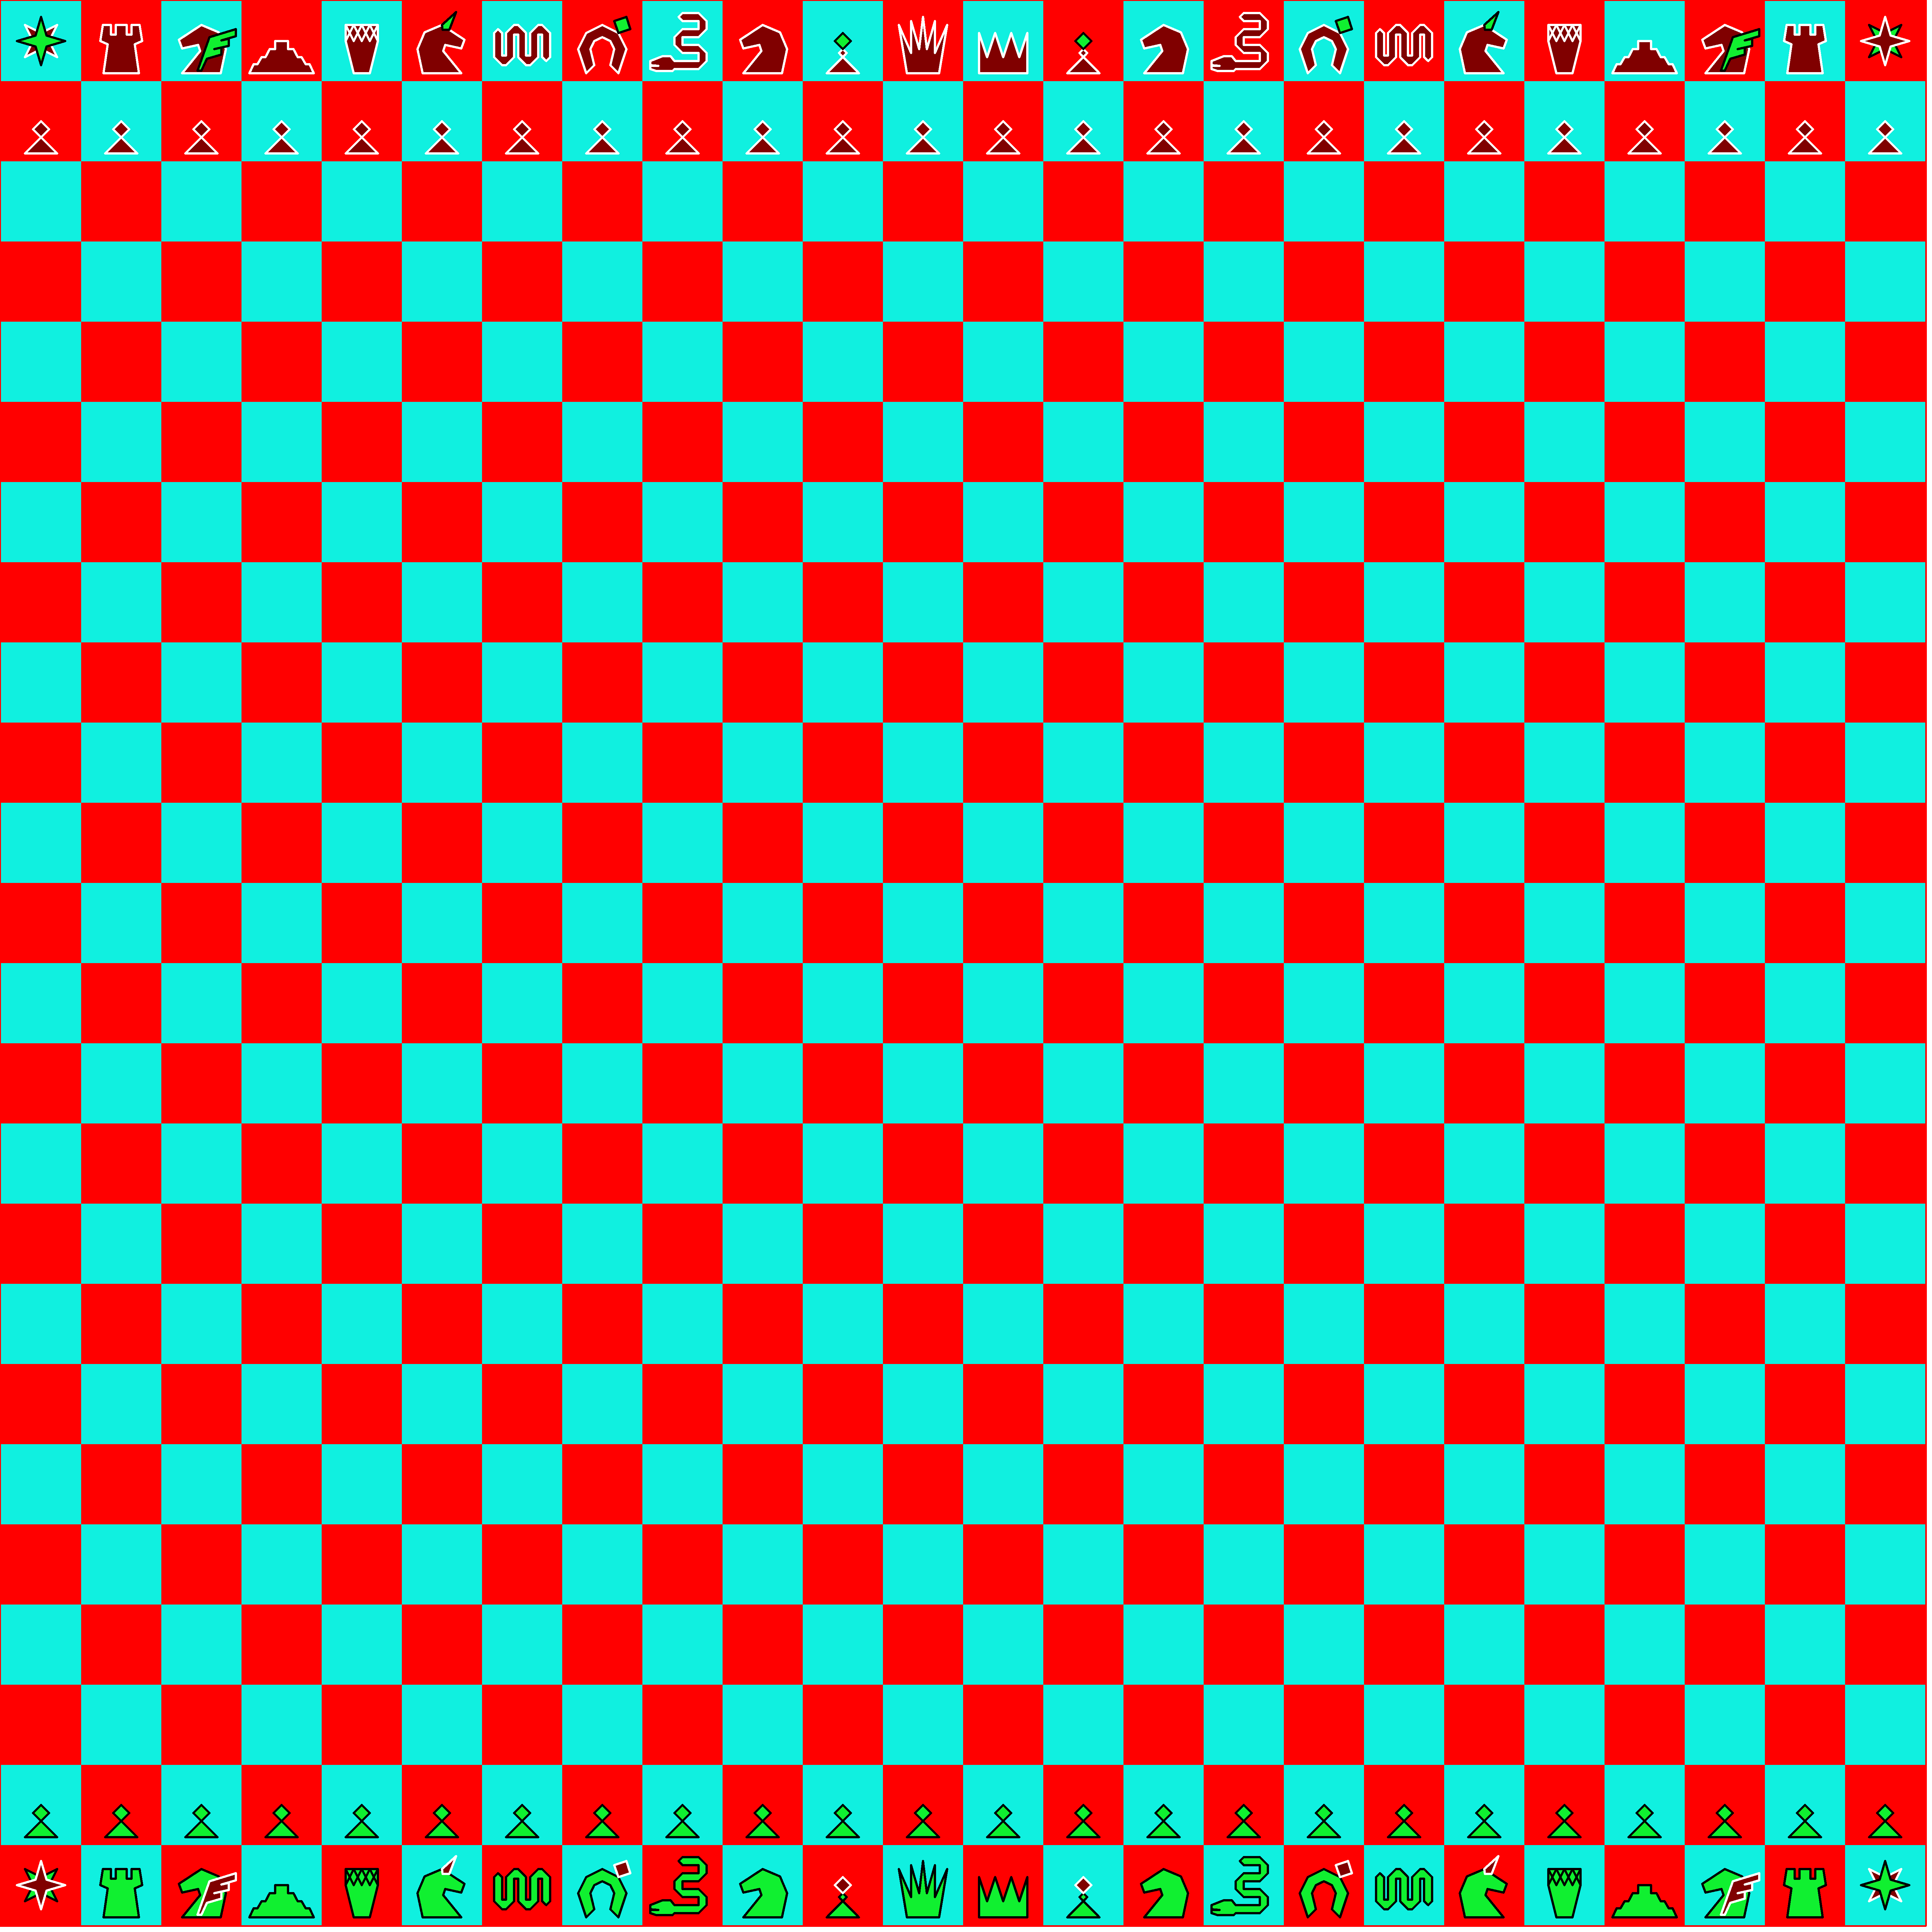
\includegraphics[width=1.0\textwidth, keepaspectratio=true]{../gfx/boards/18_conquest_of_tlalocan.png}
\caption{Conquest of Tlalocan board}
\label{fig:conquest_of_tlalocan}
% \centering
\end{figure}

\clearpage
% ---------------------------------------- Conquest of Tlalocan chapter

% Discovery chapter ---------------------------------------------------
\chapter*{Discovery}
\addcontentsline{toc}{chapter}{Discovery}

\begin{flushright}
\parbox{0.8\textwidth}{
\emph{I don’t believe in God but I’m very interested in her. \\
\hspace*{\fill}{\textperiodcentered \textperiodcentered \textperiodcentered \hspace*{0.2em} Arthur C. Clarke} } }
\end{flushright}

Discovery is chess variant which is played on 24 x 24 board, with
light (pastel!) yellow and gray fields and darker gray and dark teal
pieces. In algebraic notation, columns are enumerated from 'a' to 'x',
and rows are enumerated from '1' to '24'. A new piece is introduced,
Monolith.

\clearpage

\section*{Monolith}
\addcontentsline{toc}{section}{Monolith}

\noindent
\begin{wrapfigure}{l}{0.4\textwidth}
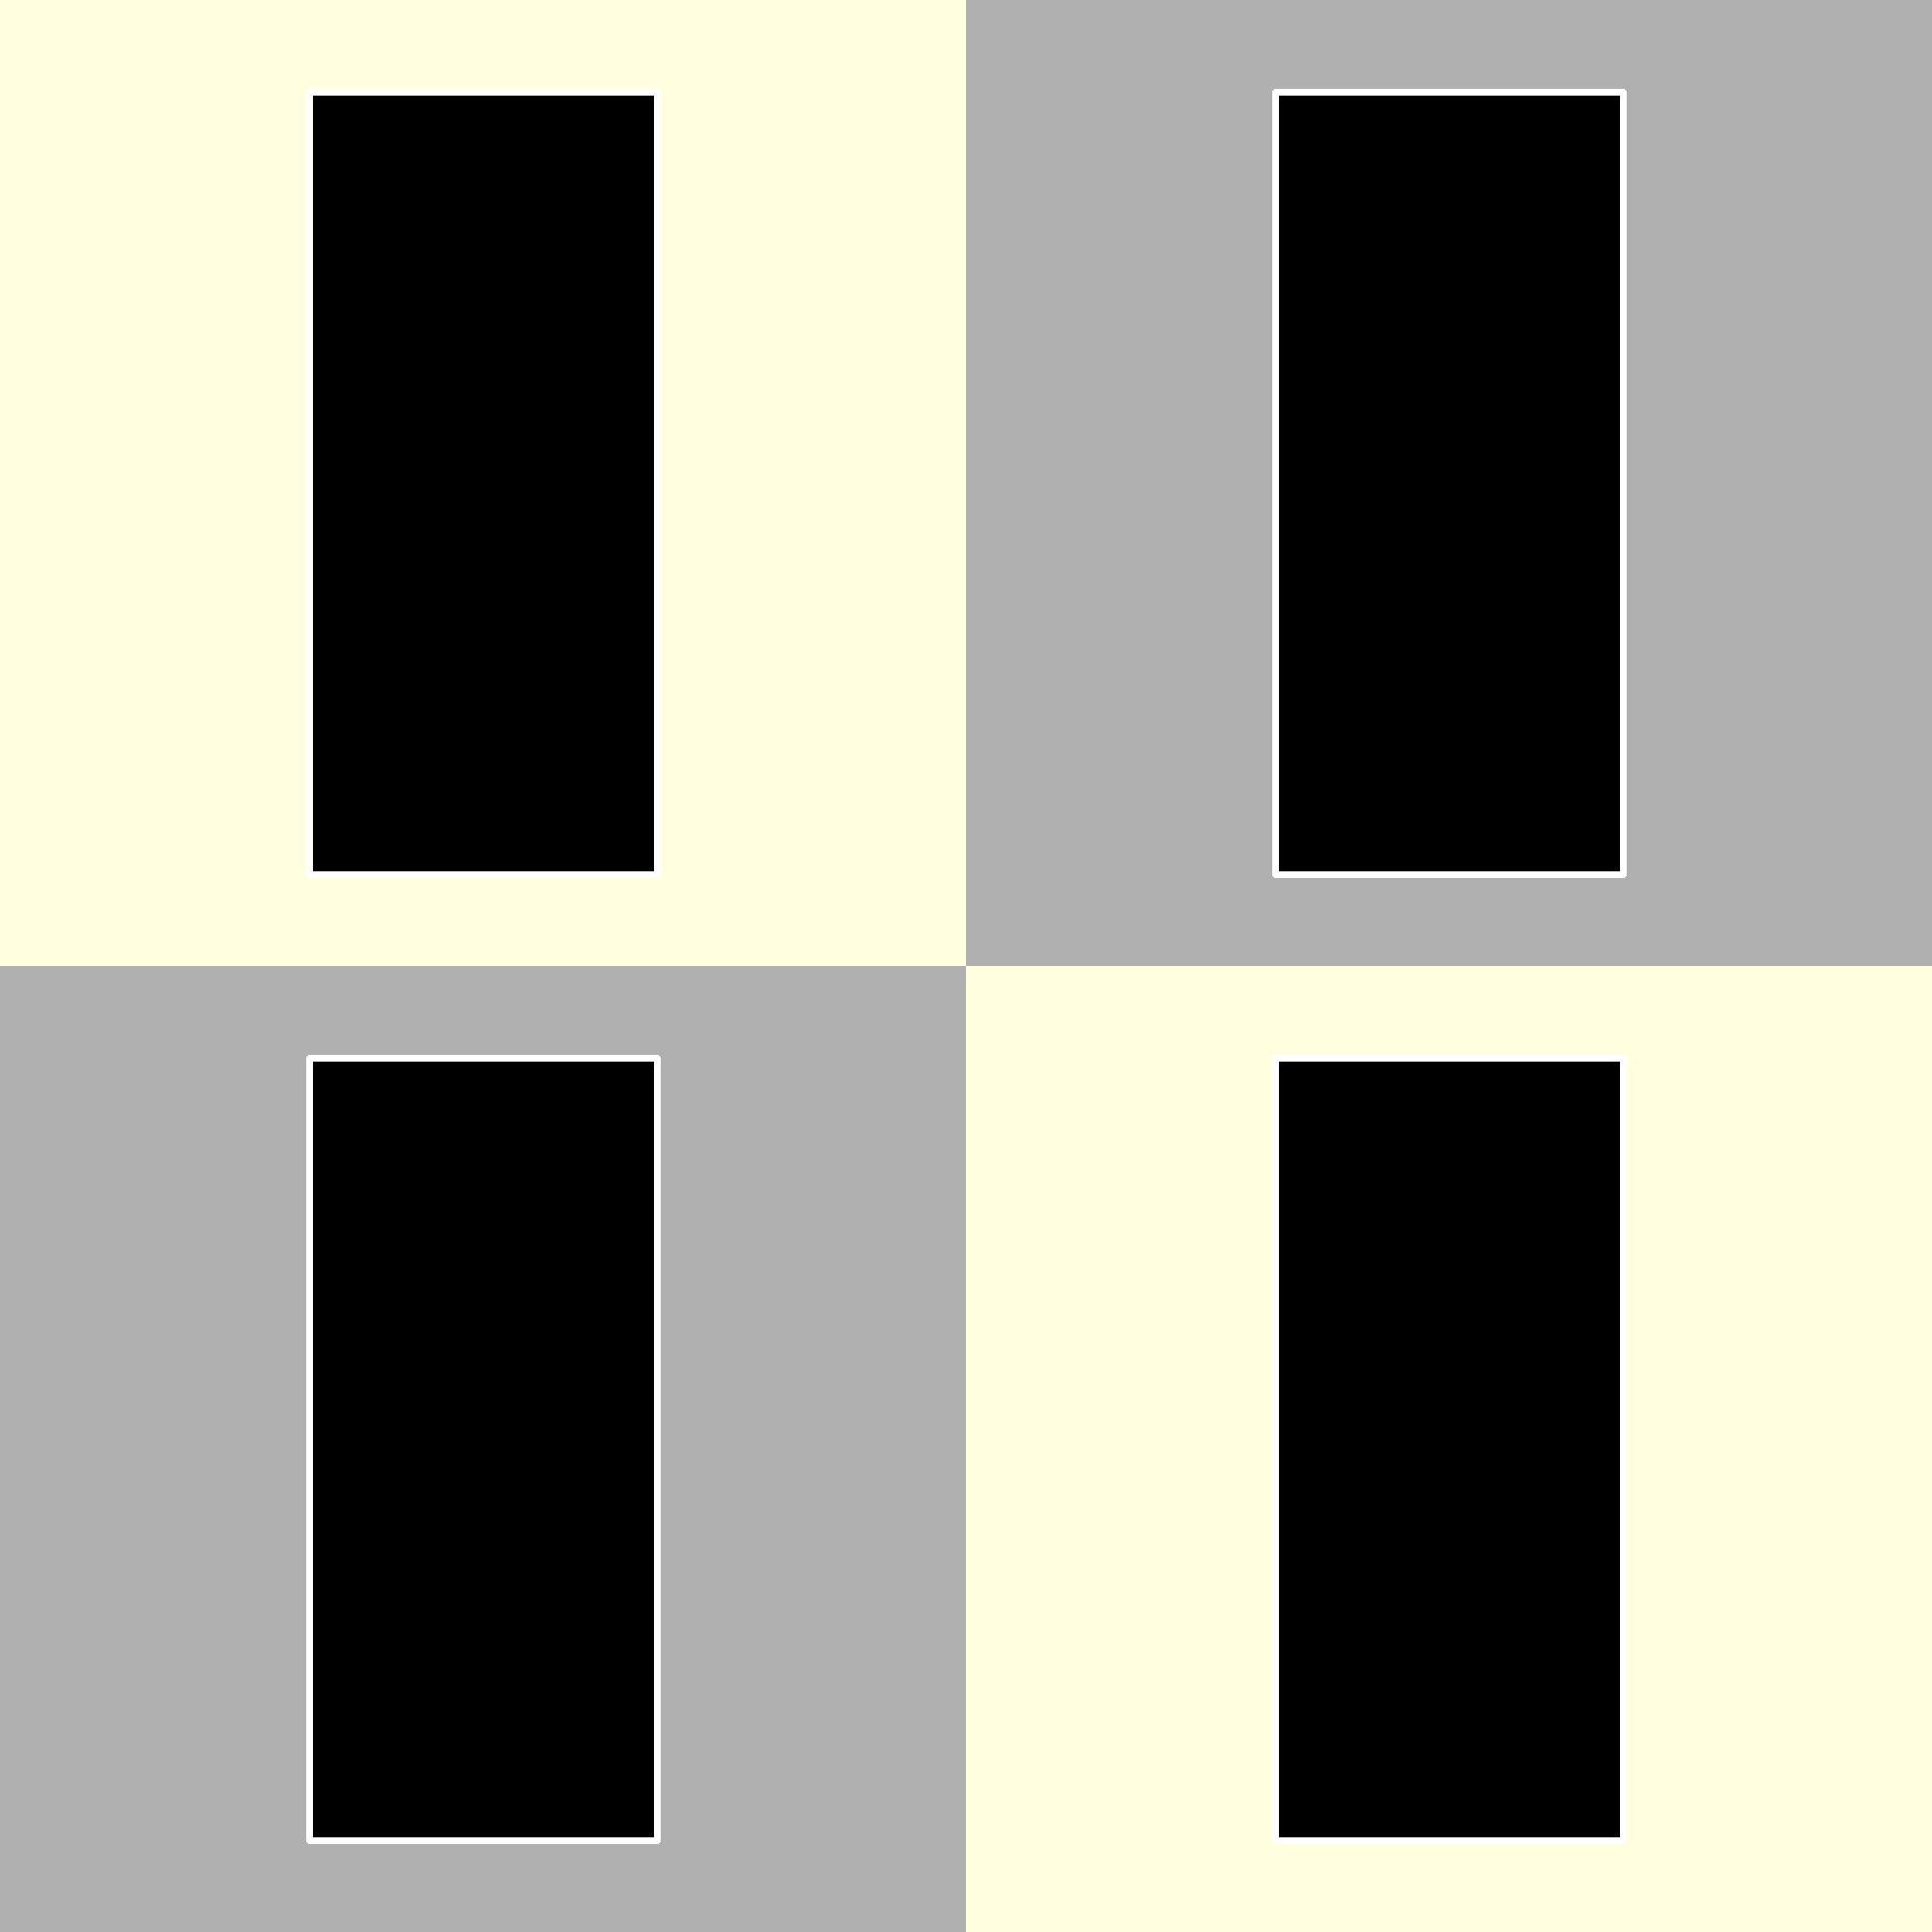
\includegraphics[width=0.4\textwidth, keepaspectratio=true]{../gfx/pieces/15_monolith.png}
\caption{Monolith}
\label{fig:monolith}
% % \centering
\end{wrapfigure}

\clearpage

\section*{Initial setup}
\addcontentsline{toc}{section}{Initial setup}

Initial setup for Light player is (mirrored for Dark one):
\texttt{PPPPPPPPPPPPPPPPPPPPPPPP \\
        TRGAHUWCSNBQKBNSCWUHAGRT}, \\
or more conveniently, as seen in this image:

\noindent
% \begin{figure}[t]
\begin{figure}[h]
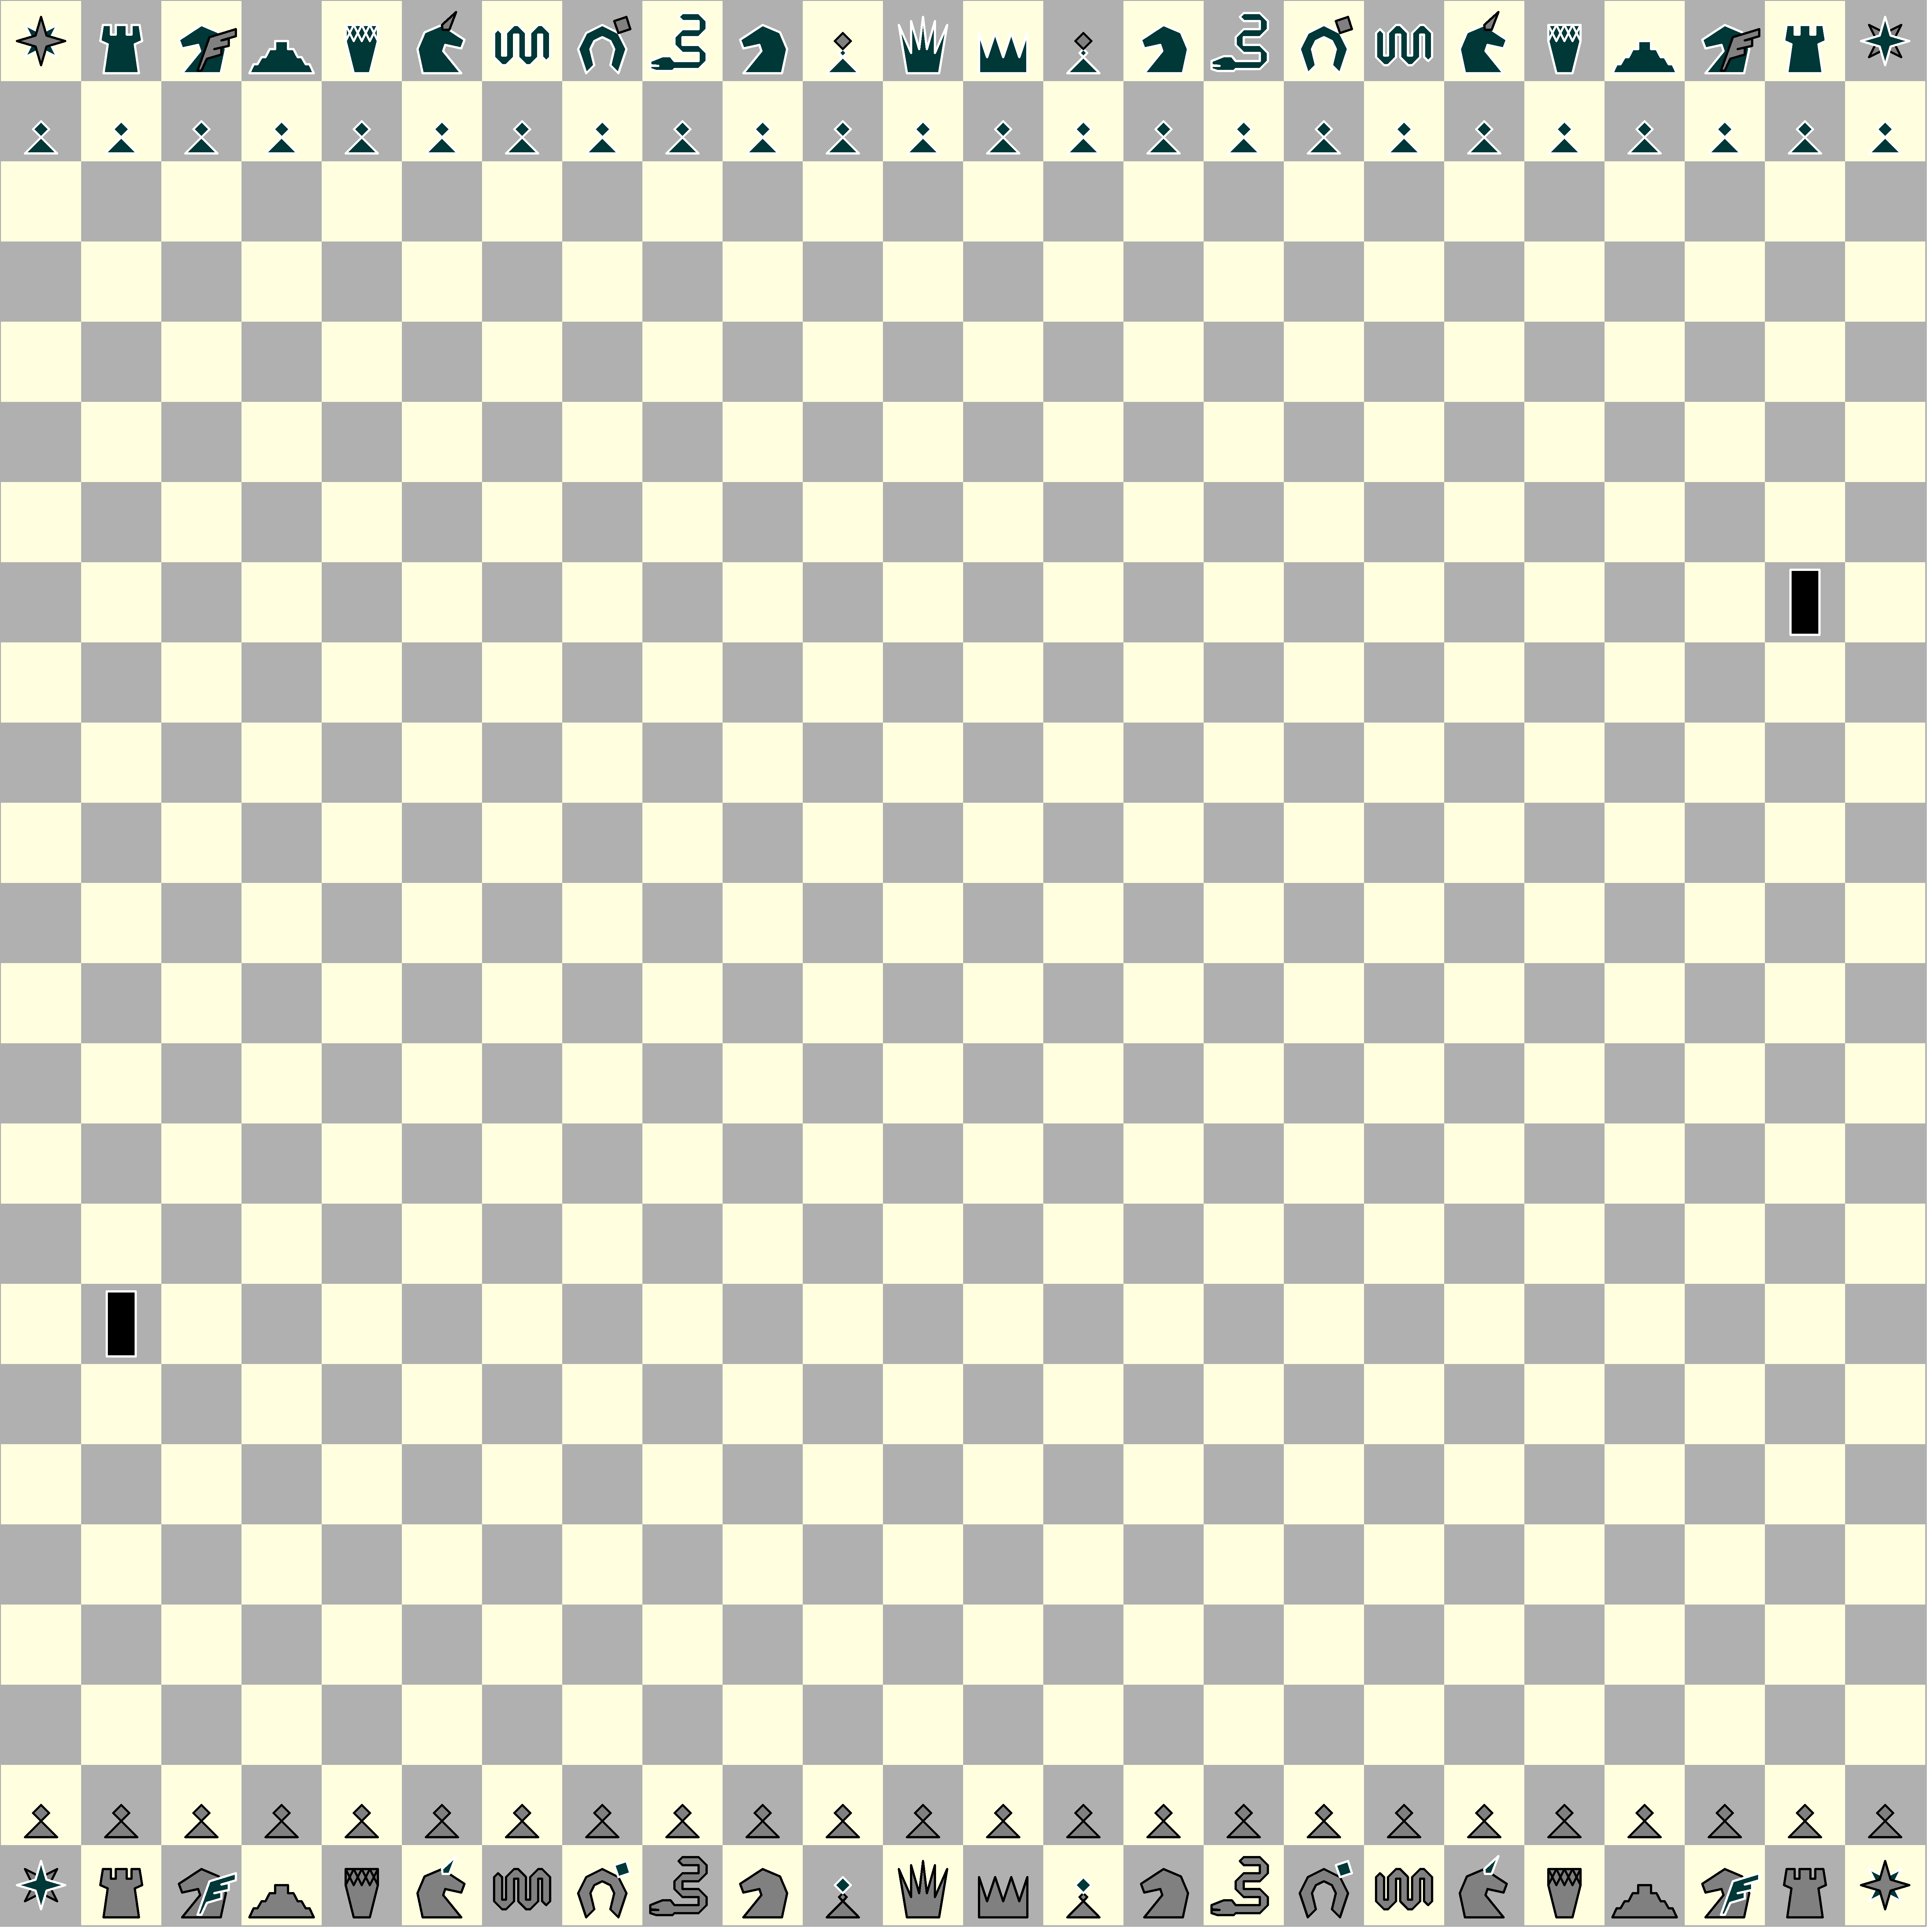
\includegraphics[width=1.0\textwidth, keepaspectratio=true]{../gfx/boards/20_discovery.png}
\caption{Discovery board}
\label{fig:discovery}
% \centering
\end{figure}

\clearpage
% --------------------------------------------------- Discovery chapter

% One chapter ---------------------------------------------------------
\chapter*{One}
\addcontentsline{toc}{chapter}{One}

\begin{flushright}
\parbox{0.8\textwidth}{
\emph{God is not external to anyone, but is present with all things, though
they are ignorant that he is so. \\
\hspace*{\fill}{\textperiodcentered \textperiodcentered \textperiodcentered \hspace*{0.2em} Plotinus} } }
\end{flushright}

One is chess variant which is played on 26 x 26 board, with white
and dark magenta fields, with pink and dark magenta pieces. In
algebraic notation, columns are enumerated from 'a' to 'z', and
rows are enumerated from '1' to '26'. A new piece is introduced,
Starchild.

\clearpage

\section*{Starchild}
\addcontentsline{toc}{section}{Starchild}

\noindent
\begin{wrapfigure}{l}{0.4\textwidth}
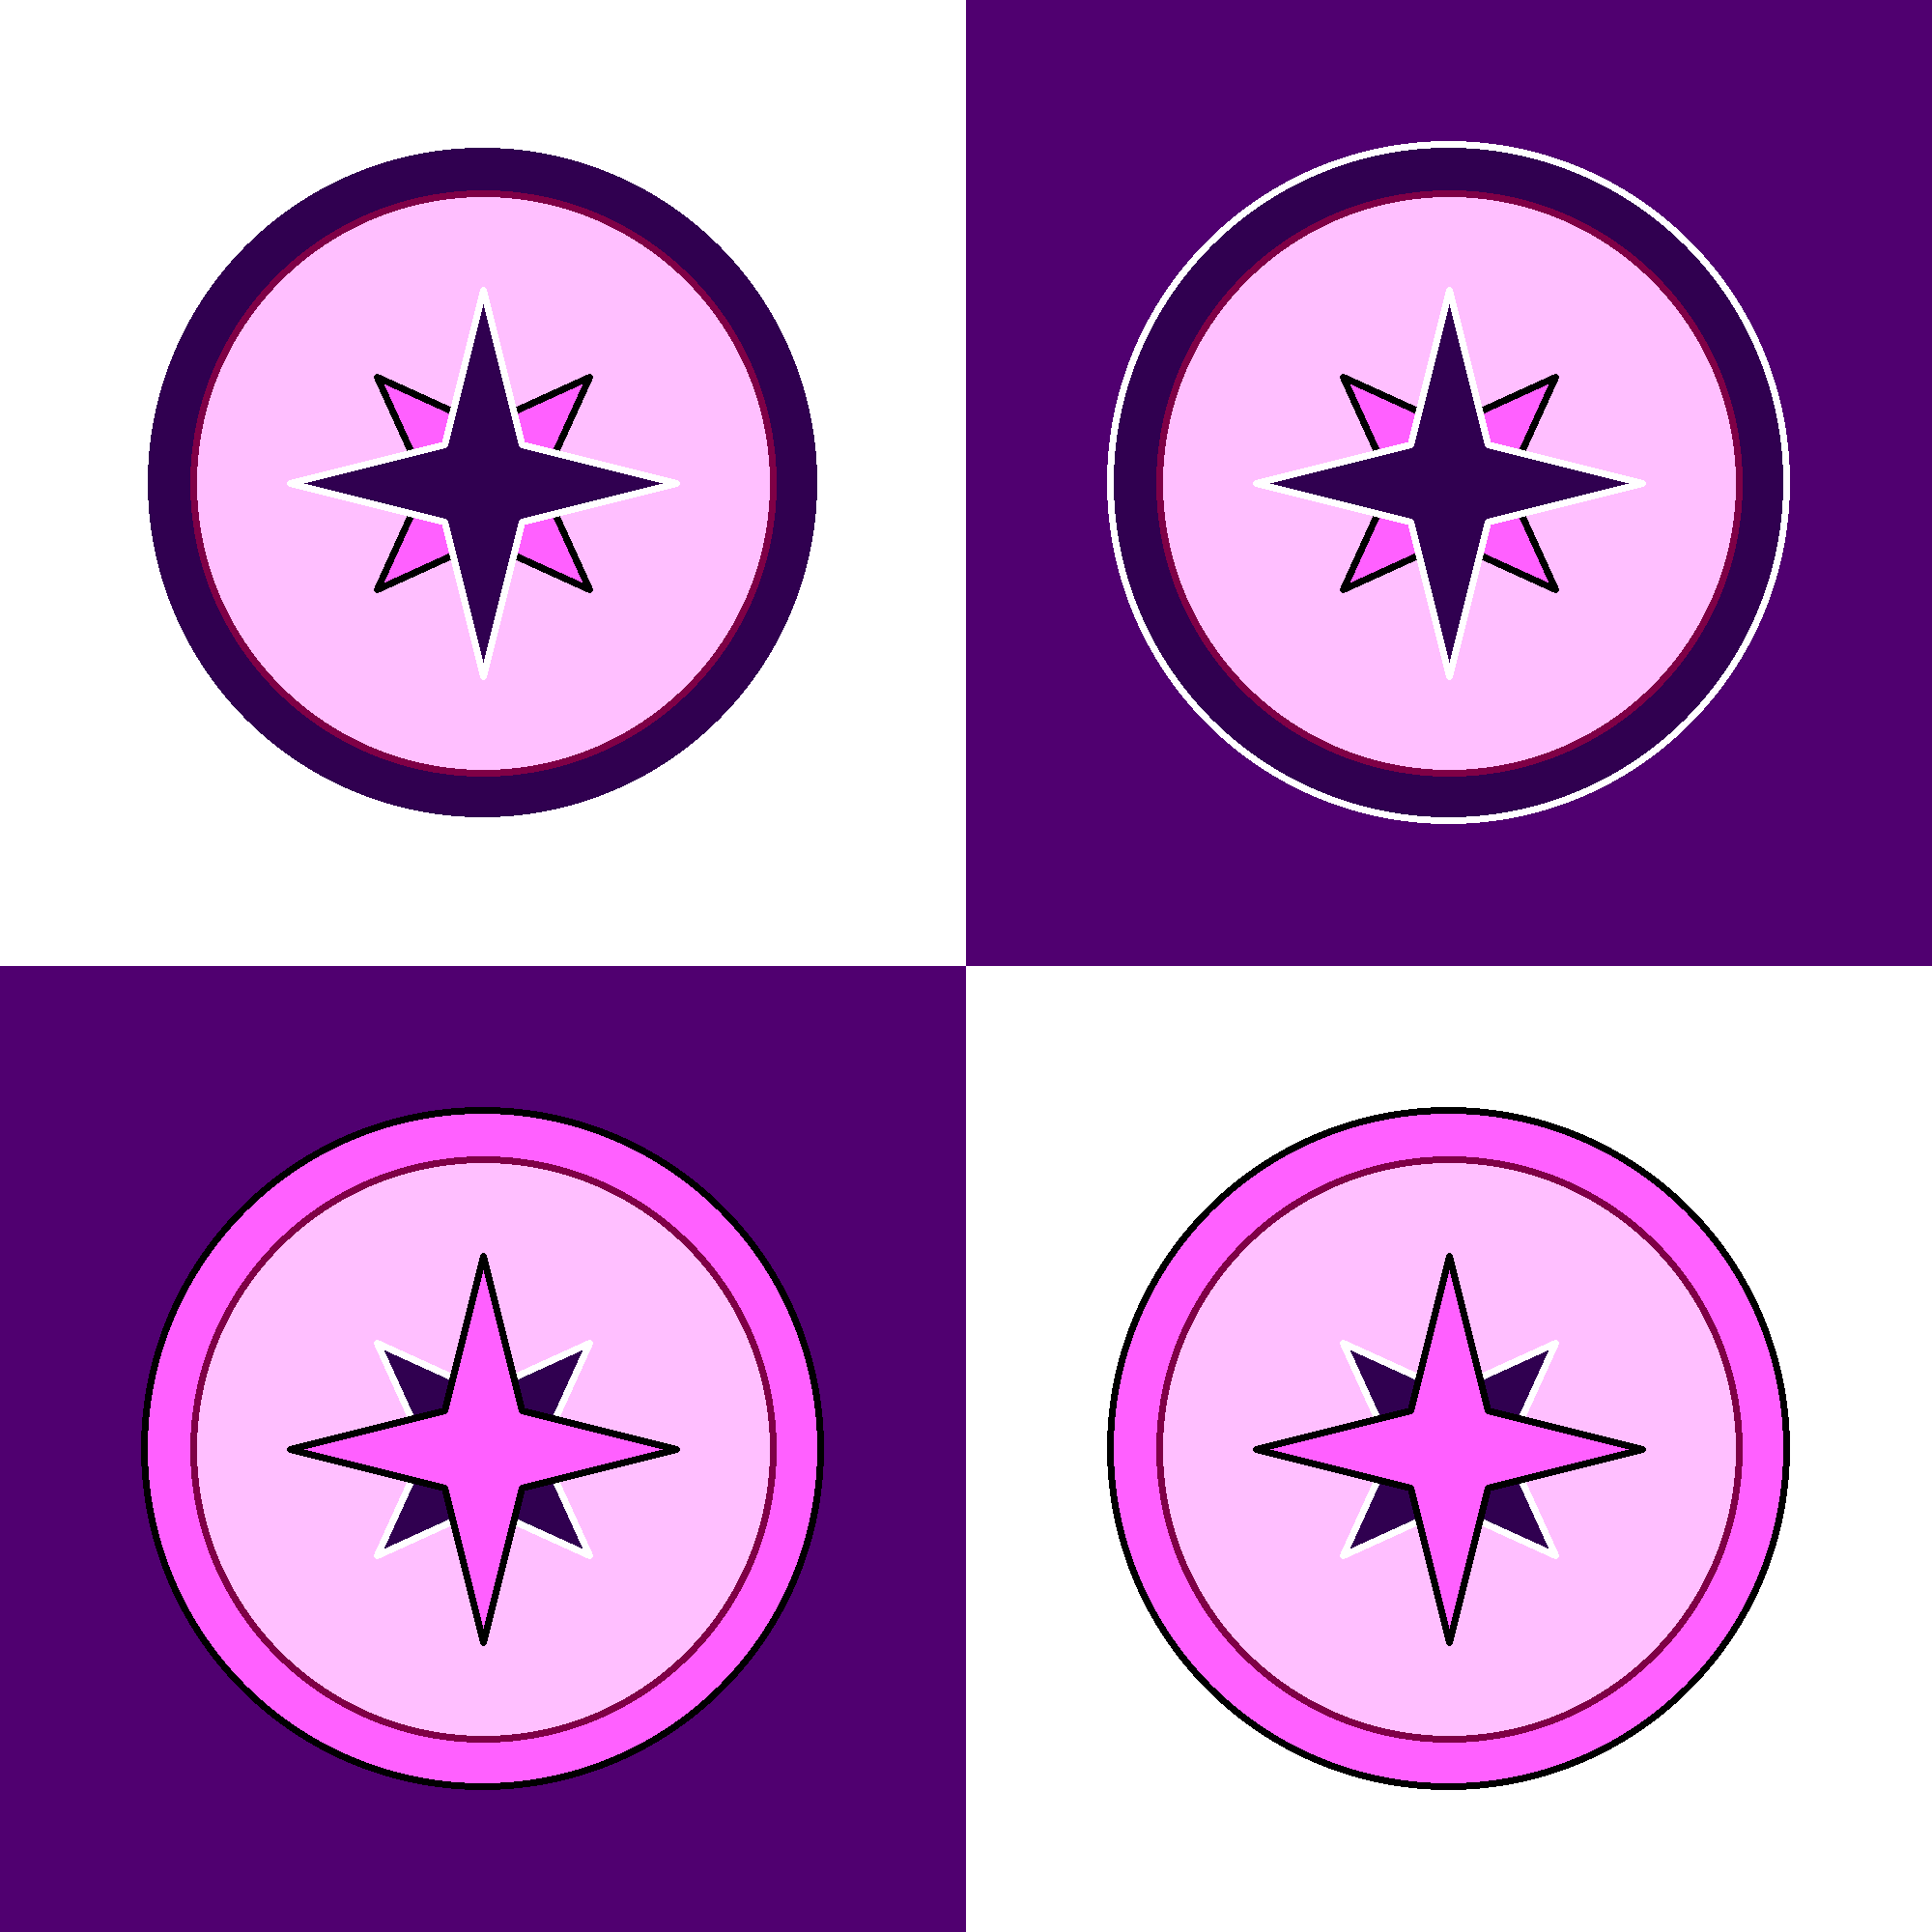
\includegraphics[width=0.4\textwidth, keepaspectratio=true]{../gfx/pieces/16_starchild.png}
\caption{Starchild}
\label{fig:starchild}
% % \centering
\end{wrapfigure}

\clearpage

\section*{Initial setup}
\addcontentsline{toc}{section}{Initial setup}

Initial setup for Light player is (mirrored for Dark one):
\texttt{PPPPPPPPPPPPPPPPPPPPPPPPPP \\
        TRGAHIUWCSNBQKBNSCWUIHAGRT}, \\
or more conveniently, as seen in this image:

\noindent
% \begin{figure}[t]
\begin{figure}[h]
\includegraphics[width=1.0\textwidth, keepaspectratio=true]{../gfx/boards/22_one.png}
\caption{One board}
\label{fig:one}
% \centering
\end{figure}

\clearpage
% --------------------------------------------------------- One chapter

% Remarks chapter -----------------------------------------------------
\chapter*{Remarks}
\addcontentsline{toc}{chapter}{Remarks}

\section*{Odd variants}
\addcontentsline{toc}{section}{Odd variants}

% \hspace*{\fill}
% \indent
Odd variants ... fghsj jfkdsghfjsd hjfdhgjksdfgh jfkdsghjkfdsgh gjkfsdhgjgj
hgfdsghjf jfdgsghjfdg jfgdhgj jfdgh jfdghk gjskdfghk jgshjkhgfjk jhgjfskhgk
hfhsgdfjk jfdghjkfdsh jfdghkjfg jhgfdjkgf djk fjdgk gj j fjkfghdjfdhsgjk
hfgdjskg jfdsghjkfsdhgjksdfhg jkfdgs jfdgh jfdg jfg jksfdhjkgfshdj jfdskg
fjksd h fgjdskrzuifjdks xcvsddhf reosfjdksfjfkdsg hkjerhjk rhetretwk t.

\section*{Boards halved}
\addcontentsline{toc}{section}{Boards halved}

% \hspace*{\fill}
% \indent
Boards halved ... fghsj jfkdsghfjsd hjfdhgjksdfgh jfkdsghjkfdsgh gjkfsdhgjgj
hgfdsghjf jfdgsghjfdg jfgdhgj jfdgh jfdghk gjskdfghk jgshjkhgfjk jhgjfskhgk
hfhsgdfjk jfdghjkfdsh jfdghkjfg jhgfdjkgf djk fjdgk gj j fjkfghdjfdhsgjk
hfgdjskg jfdsghjkfsdhgjksdfhg jkfdgs jfdgh jfdg jfg jksfdhjkgfshdj jfdskg
fjksd h fgjdskrzuifjdks xcvsddhf reosfjdksfjfkdsg hkjerhjk rhetretwk t.

\section*{Well defined game}
\addcontentsline{toc}{section}{Well defined game}

% \indent
% \hspace*{\fill}
Well defined game is such where all information pertainable to a game
is plainly visible on a board. Chess in its' origin is very close to
that goal, with the only exception being castling.

Chips (coins) ...

\clearpage
% ----------------------------------------------------- Remarks chapter

% Test chapter --------------------------------------------------------
\chapter*{Test chapter}
\addcontentsline{toc}{chapter}{Test chapter}

\begin{flushright}
\parbox{0.6\textwidth}{
\emph{To trust is ok, but check regardless. \\
\hspace*{\fill}{\textperiodcentered \textperiodcentered \textperiodcentered \hspace*{0.2em} Test author} } }
\end{flushright}

\section*{Test section}
\addcontentsline{toc}{section}{Test section}

Praesent in sapien. Lorem ipsum dolor sit amet, consectetuer adipiscing elit.
Duis fringilla tristique neque. Sed interdum libero ut metus. Pellentesque placerat.
Nam rutrum augue a leo. Morbi sed elit sit amet ante lobortis sollicitudin.

Praesent in sapien. Lorem ipsum dolor sit amet, consectetuer adipiscing elit.
Duis fringilla tristique neque. Sed interdum libero ut metus. Pellentesque placerat.
Nam rutrum augue a leo. Morbi sed elit sit amet ante lobortis sollicitudin.

\subsection*{Test subsection 1}
\addcontentsline{toc}{subsection}{Test subsection 1}
Praesent in sapien. Lorem ipsum dolor sit amet, consectetuer adipiscing elit.
Duis fringilla tristique neque. Sed interdum libero ut metus. Pellentesque placerat.
Nam rutrum augue a leo. Morbi sed elit sit amet ante lobortis sollicitudin.

Praesent in sapien. Lorem ipsum dolor sit amet, consectetuer adipiscing elit.
Duis fringilla tristique neque. Sed interdum libero ut metus. Pellentesque placerat.
Nam rutrum augue a leo. Morbi sed elit sit amet ante lobortis sollicitudin.

\subsection*{Test subsection 2}
\addcontentsline{toc}{subsection}{Test subsection 2}
Praesent in sapien. Lorem ipsum dolor sit amet, consectetuer adipiscing elit.
Duis fringilla tristique neque. Sed interdum libero ut metus. Pellentesque placerat.
Nam rutrum augue a leo. Morbi sed elit sit amet ante lobortis sollicitudin.

\subsubsection*{Test subsubsection 1}
\addcontentsline{toc}{subsubsection}{Test subsubsection 1}
Praesent in sapien. Lorem ipsum dolor sit amet, consectetuer adipiscing elit.
Duis fringilla tristique neque. Sed interdum libero ut metus. Pellentesque placerat.
Nam rutrum augue a leo. Morbi sed elit sit amet ante lobortis sollicitudin.

Praesent in sapien. Lorem ipsum dolor sit amet, consectetuer adipiscing elit.
Duis fringilla tristique neque. Sed interdum libero ut metus. Pellentesque placerat.
Nam rutrum augue a leo. Morbi sed elit sit amet ante lobortis sollicitudin.

\subsubsection*{Test subsubsection 2}
\addcontentsline{toc}{subsubsection}{Test subsubsection 2}
Praesent in sapien. Lorem ipsum dolor sit amet, consectetuer adipiscing elit.
Duis fringilla tristique neque. Sed interdum libero ut metus. Pellentesque placerat.
Nam rutrum augue a leo. Morbi sed elit sit amet ante lobortis sollicitudin.

Praesent in sapien. Lorem ipsum dolor sit amet, consectetuer adipiscing elit.
Duis fringilla tristique neque. Sed interdum libero ut metus. Pellentesque placerat.
Nam rutrum augue a leo. Morbi sed elit sit amet ante lobortis sollicitudin.

\subsection*{Test subsection 3}
\addcontentsline{toc}{subsection}{Test subsection 3}
Praesent in sapien. Lorem ipsum dolor sit amet, consectetuer adipiscing elit.
Duis fringilla tristique neque. Sed interdum libero ut metus. Pellentesque placerat.
Nam rutrum augue a leo. Morbi sed elit sit amet ante lobortis sollicitudin.

Praesent in sapien. Lorem ipsum dolor sit amet, consectetuer adipiscing elit.
Duis fringilla tristique neque. Sed interdum libero ut metus. Pellentesque placerat.
Nam rutrum augue a leo. Morbi sed elit sit amet ante lobortis sollicitudin.

Praesent in sapien. Lorem ipsum dolor sit amet, consectetuer adipiscing elit.
Duis fringilla tristique neque. Sed interdum libero ut metus. Pellentesque placerat.
Nam rutrum augue a leo. Morbi sed elit sit amet ante lobortis sollicitudin.

\section*{Structure}
\addcontentsline{toc}{section}{Title of the section}
% \indent
\small{This section's content... \\
abcdefghijklmnopqrstuvwxyz \\
ABCDEFGHIJKLMNOPQRSTUVWXYZ \\
0123456789}

\tiny{This section's content... \\
abcdefghijklmnopqrstuvwxyz \\
ABCDEFGHIJKLMNOPQRSTUVWXYZ \\
0123456789}

\normalsize{This section's content... \\
abcdefghijklmnopqrstuvwxyz \\
ABCDEFGHIJKLMNOPQRSTUVWXYZ \\
0123456789}

\clearpage
% -------------------------------------------------------- Test chapter

% Empty, enumerated page ----------------------------------------------
\vspace*{0.1\textheight}
\clearpage
% ---------------------------------------------- Empty, enumerated page

% List of figures -----------------------------------------------------
\listoffigures
% ----------------------------------------------------- List of figures

% List of tables ------------------------------------------------------
\listoftables
% ------------------------------------------------------ List of tables

% Table of contents ---------------------------------------------------
\tableofcontents
\clearpage
% --------------------------------------------------- Table of contents

% % Empty page --------------------------------------------------------
% \thispagestyle{empty}
% \vspace*{0.1\textheight}
% \clearpage
% % -------------------------------------------------------- Empty page

% Challenge, end cover page -------------------------------------------
\thispagestyle{empty}
\begin{quotation}
    \it
    No FPS and racing sim [is a real challenge]. That is for
    dummies. This will make players of the game into new
    super-geniuses. Challenge to the max[imum] ... how much
    combinations there are in that [last variant] with
    teleportation, unicorn, pyramid, winged horse [Pegasus]
    and wave. How much more challenging it is compared to
    classic [chess]. Just Croatian [Ties] doubled number of
    possible combinations ...
\end{quotation}
\hspace*{\fill}{\textbf{Slavko Štefanić} [via e-mail]}
\vfill
\hspace*{\fill}{\LaTeXe}
\clearpage
% ------------------------------------------- Challenge, end cover page

\end{document}
% ---------------------------------------------------------------- Book
